\chapter{Drone Building}
In order to get familiar with the drone building process, it is highly recommended to follow this tutorial \cite{udemy_build_course}.

\section{Soldering}
For soldering you will need to have:
\begin{itemize}
    \item the frame Kit, the bottom plate (i.e. PDB).
    \item 4 ESCs
    \item 4 motors
\end{itemize}
The sequence of steps that have to be followed are:
\begin{enumerate}
    \item Put solder on the electrodes of the PDB and the ESCs.
    \item Trim off some insulation if there is not enough wire exposed.
    \item Put solder on the wires of the ESCs, motors and battery connector.
    \item Solder the 3 motor cables to each of the ESCs. Later, you will only have to inverse two pair of cables to inverse the motor rotation. {\color{orange} Elaborate}
    \item Solder the battery and connect the ESCs to the PDB.
\end{enumerate}
\begin{figure}[!ht]
    \centering
    \begin{subfigure}[b]{0.3\textwidth}
        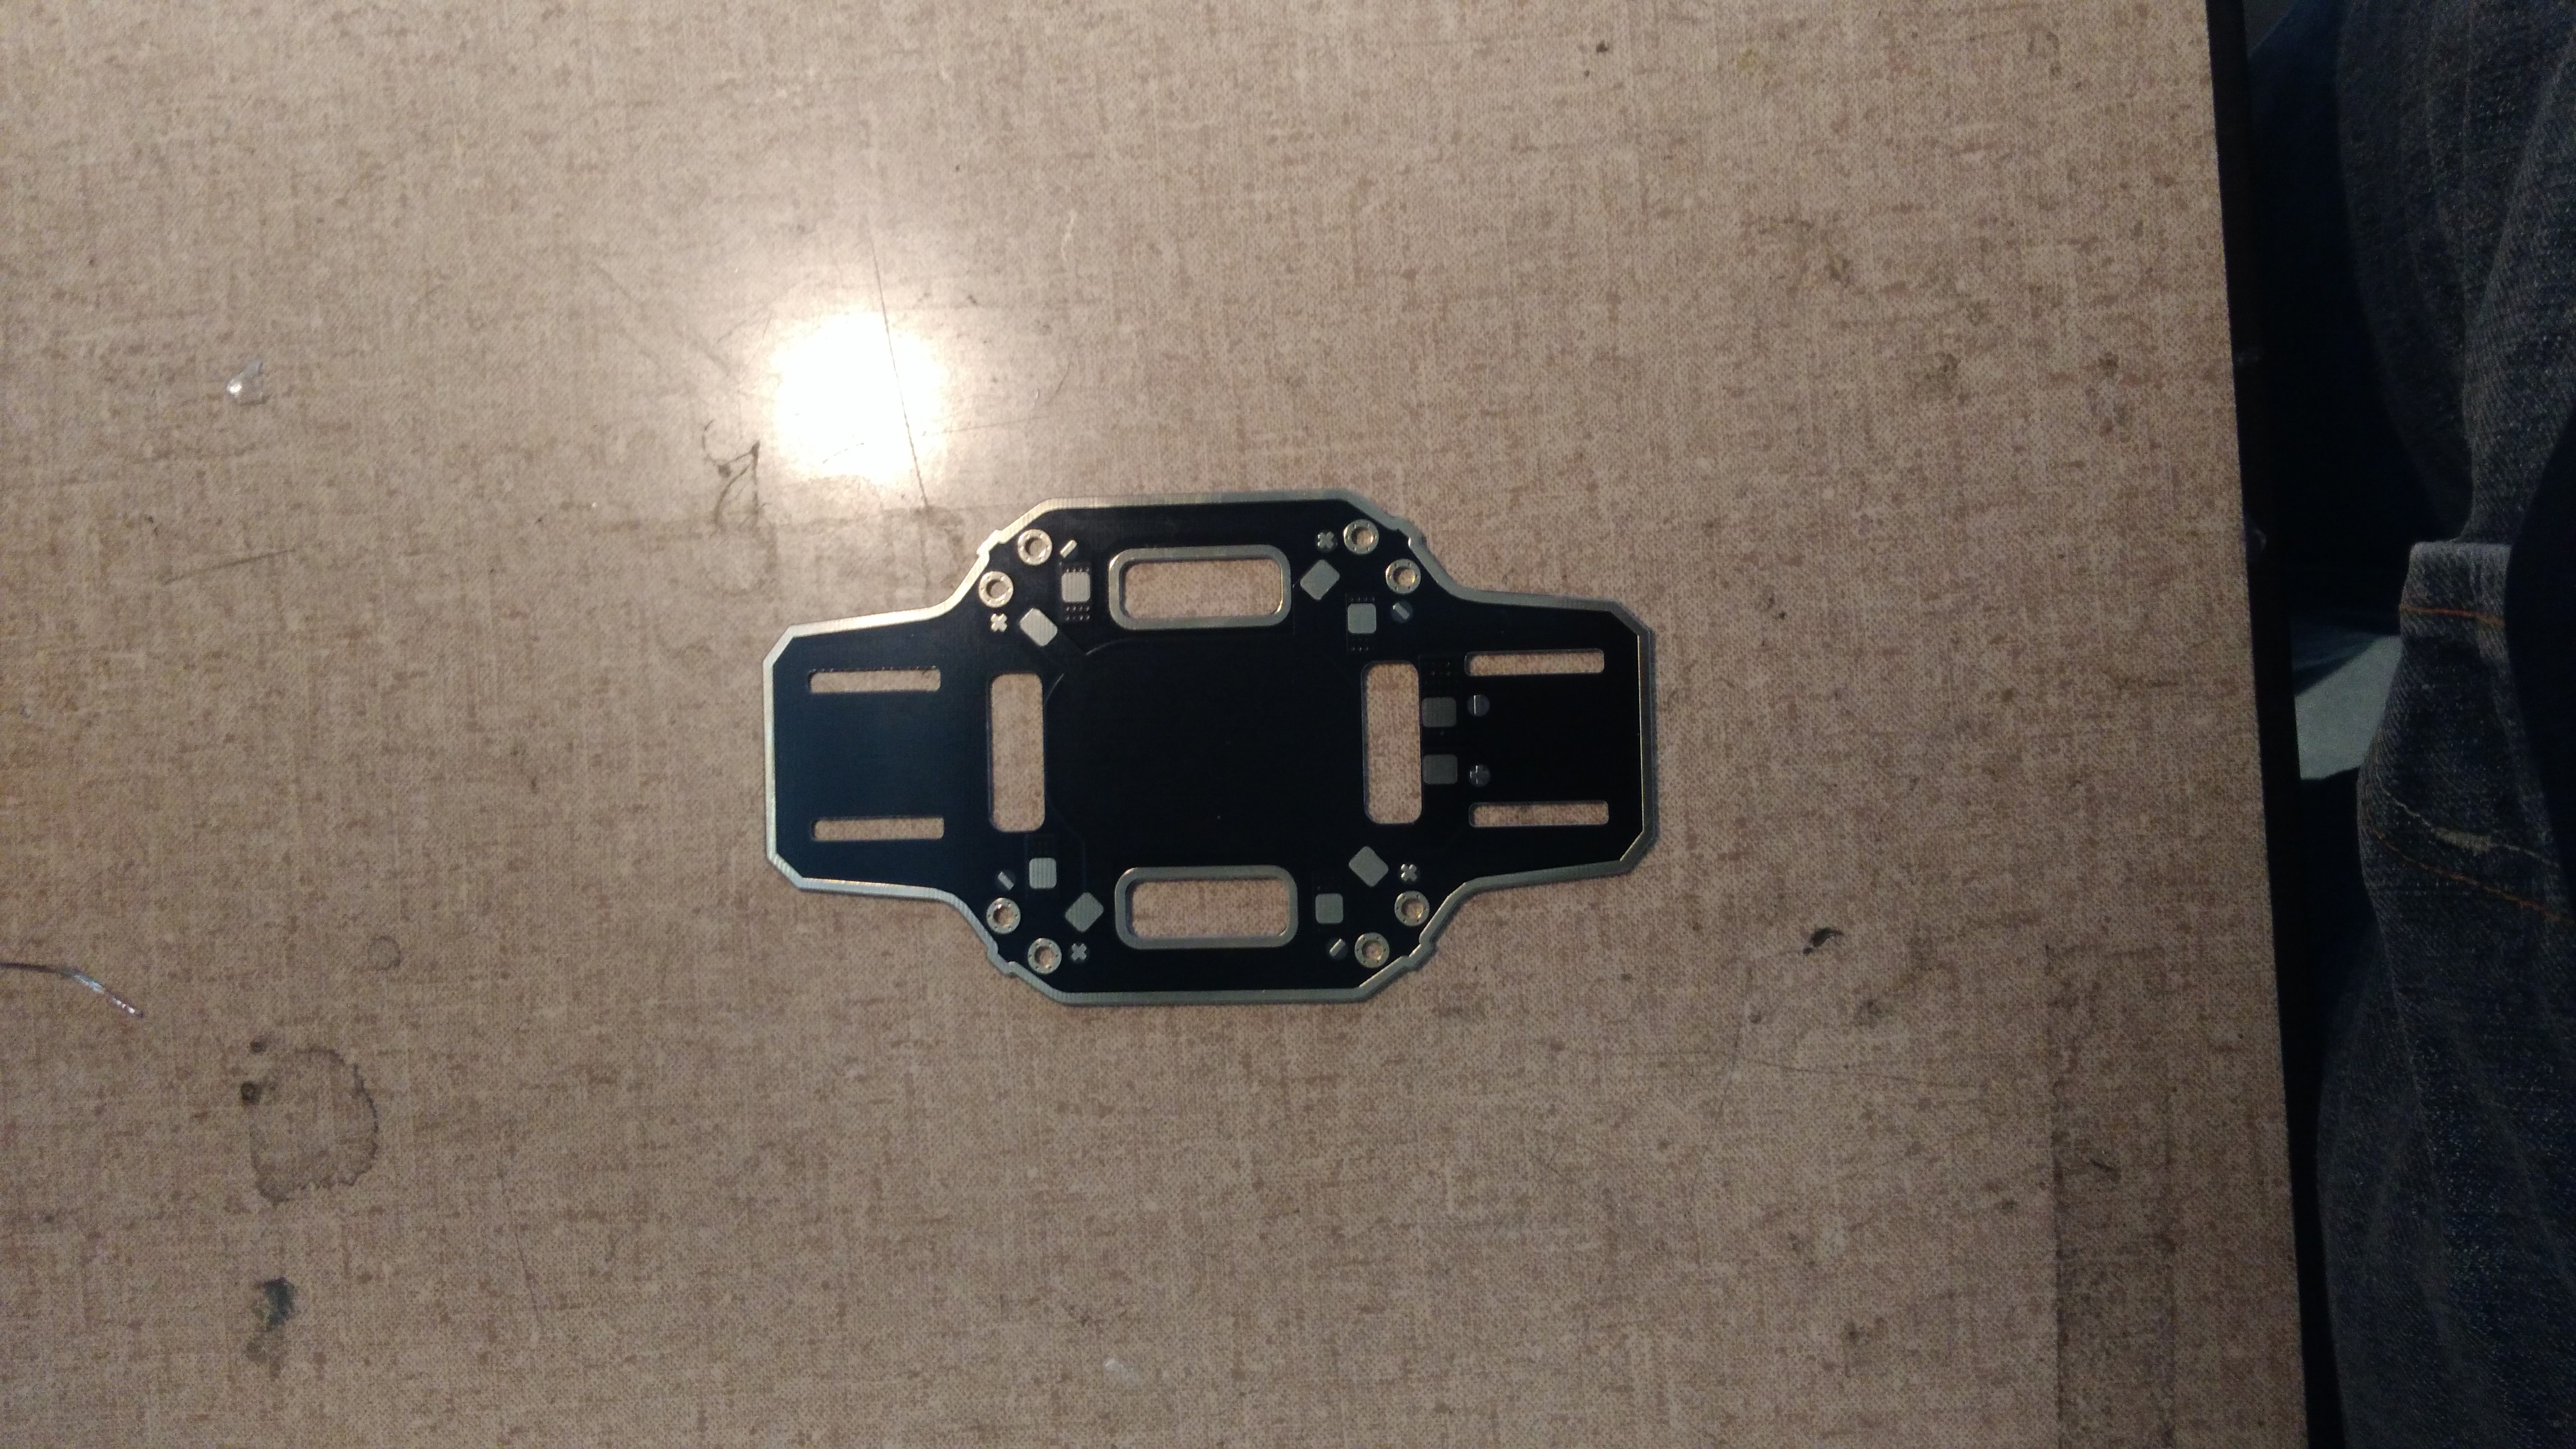
\includegraphics[width=\textwidth]{building/pdb.jpg}
        \caption{Start}
        \label{fig:pdb}
    \end{subfigure}
    ~
    \begin{subfigure}[b]{0.3\textwidth}
        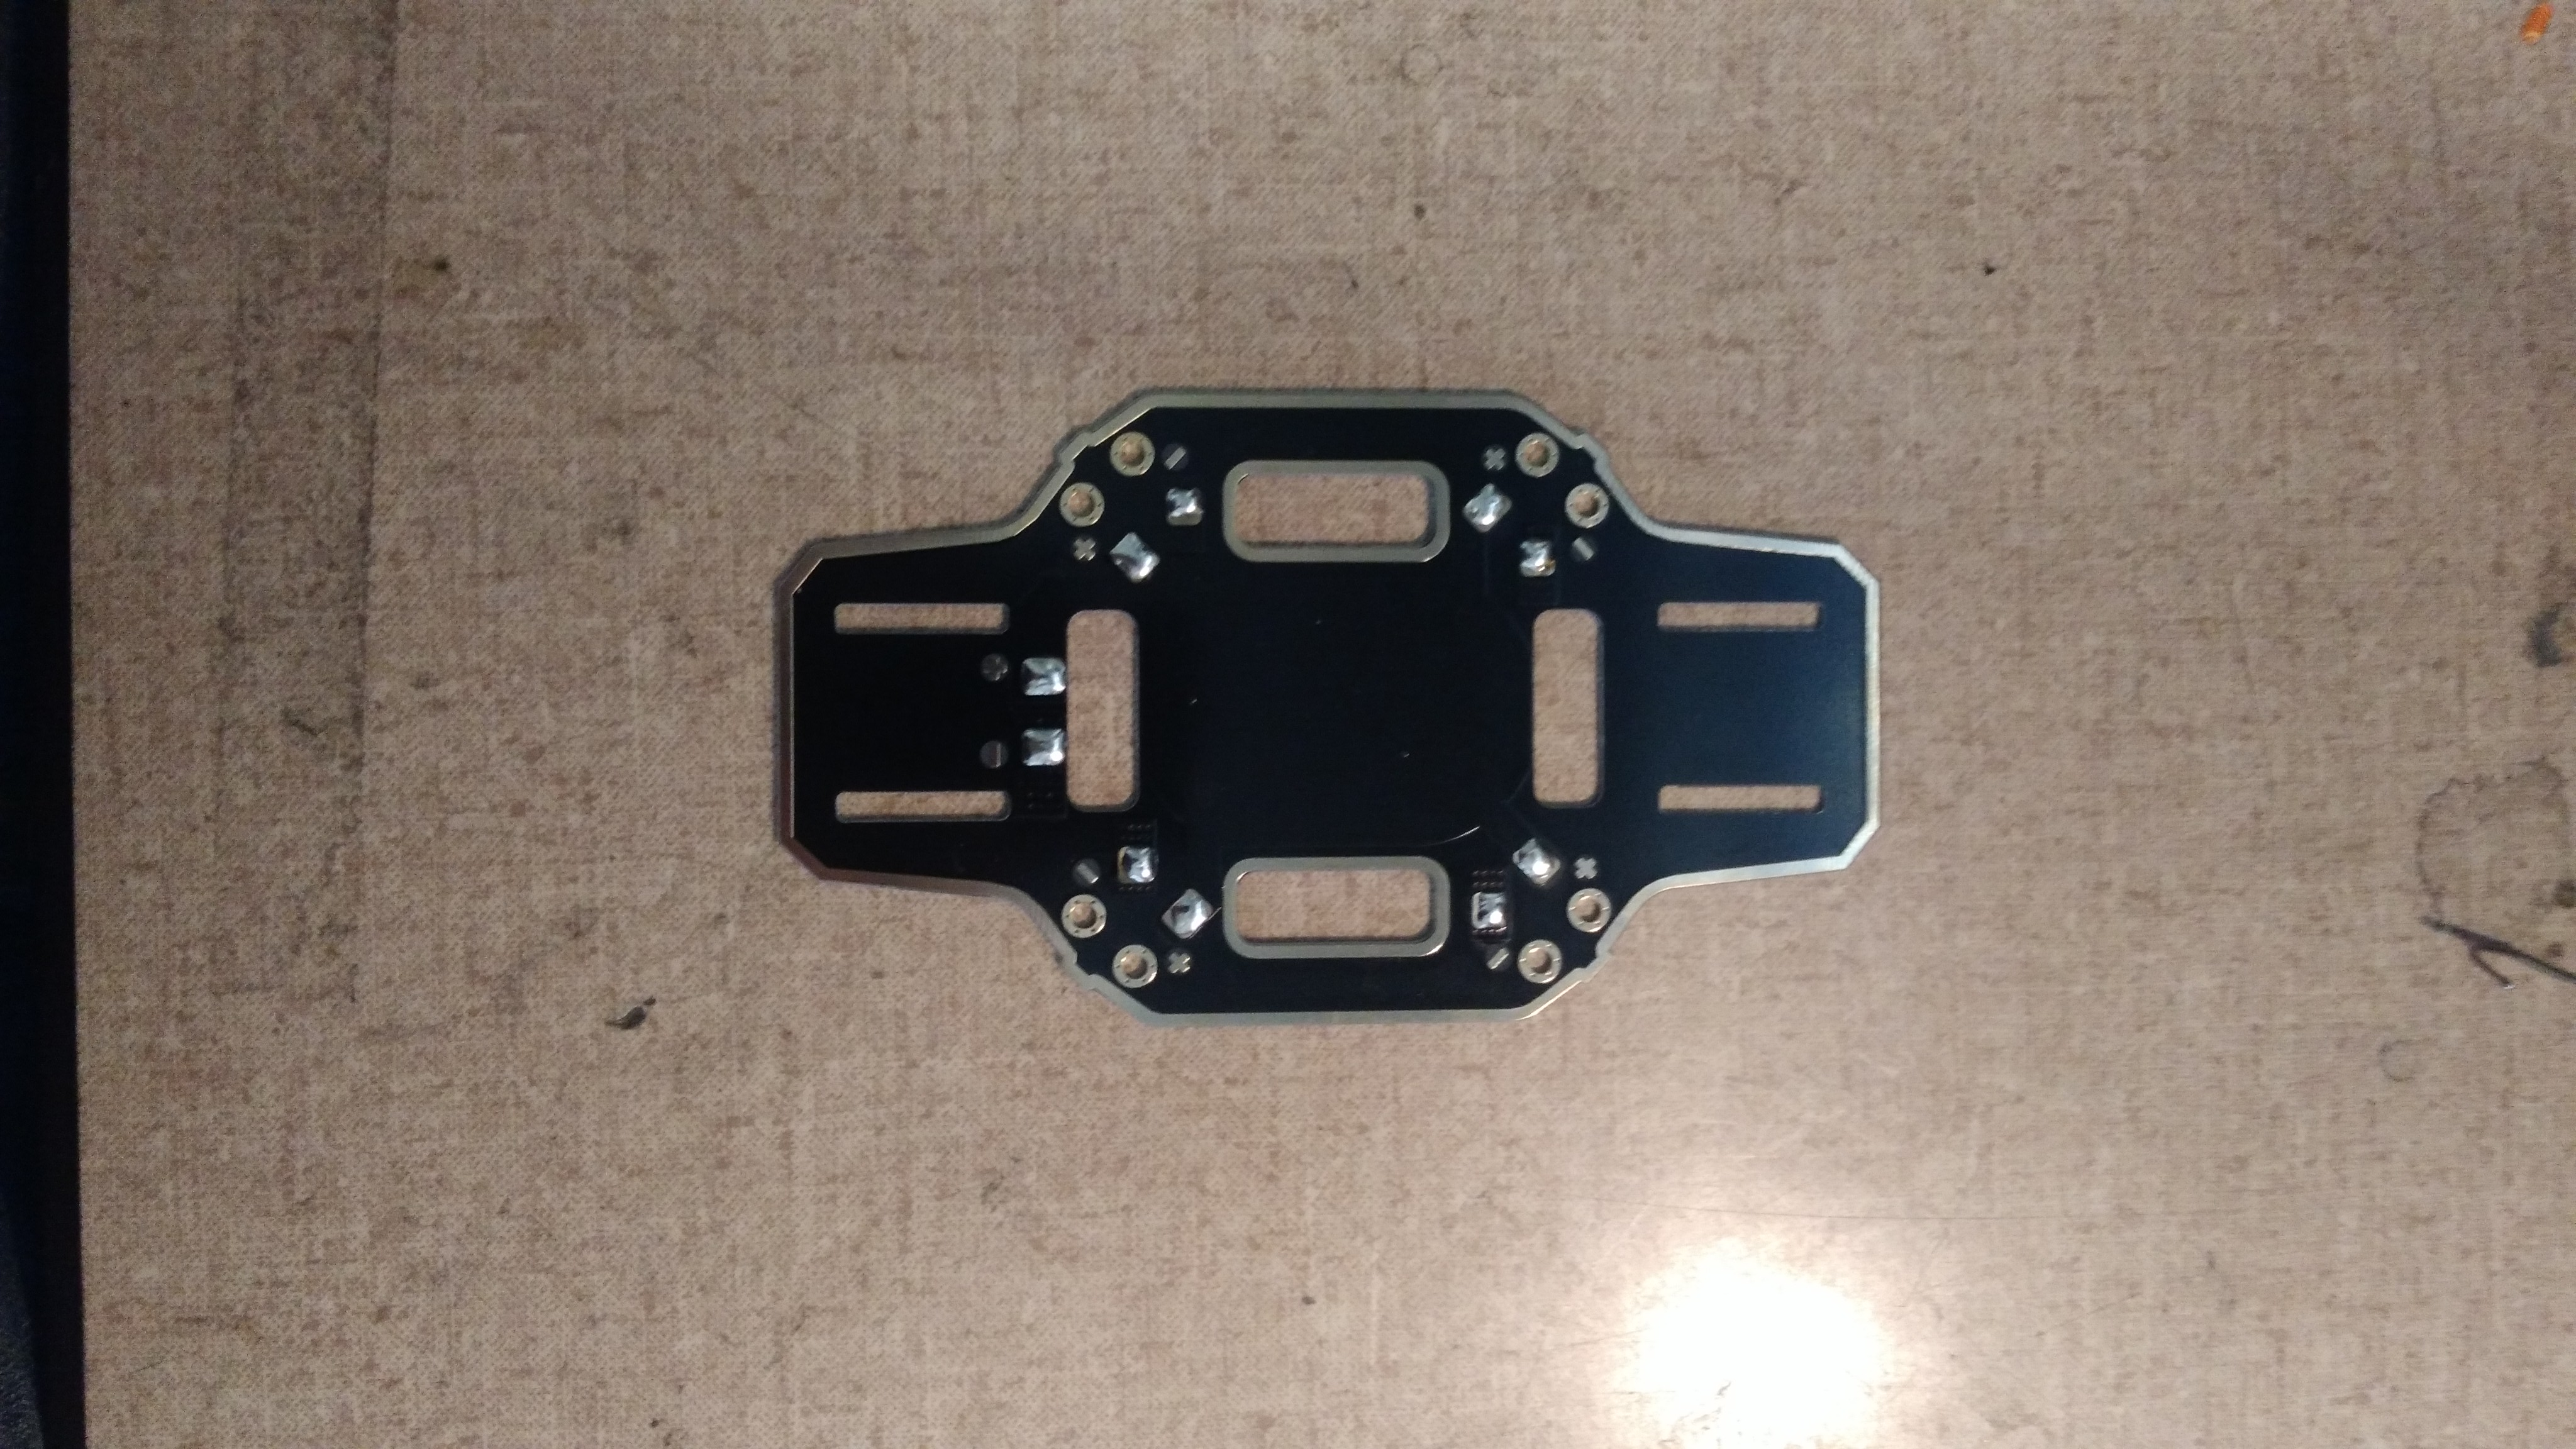
\includegraphics[width=\textwidth]{building/pdb_electrodes_solder.jpg}
        \caption{Put solder}
        \label{fig:pdb_electrodes_solder}
    \end{subfigure}
    ~
    \begin{subfigure}[b]{0.3\textwidth}
        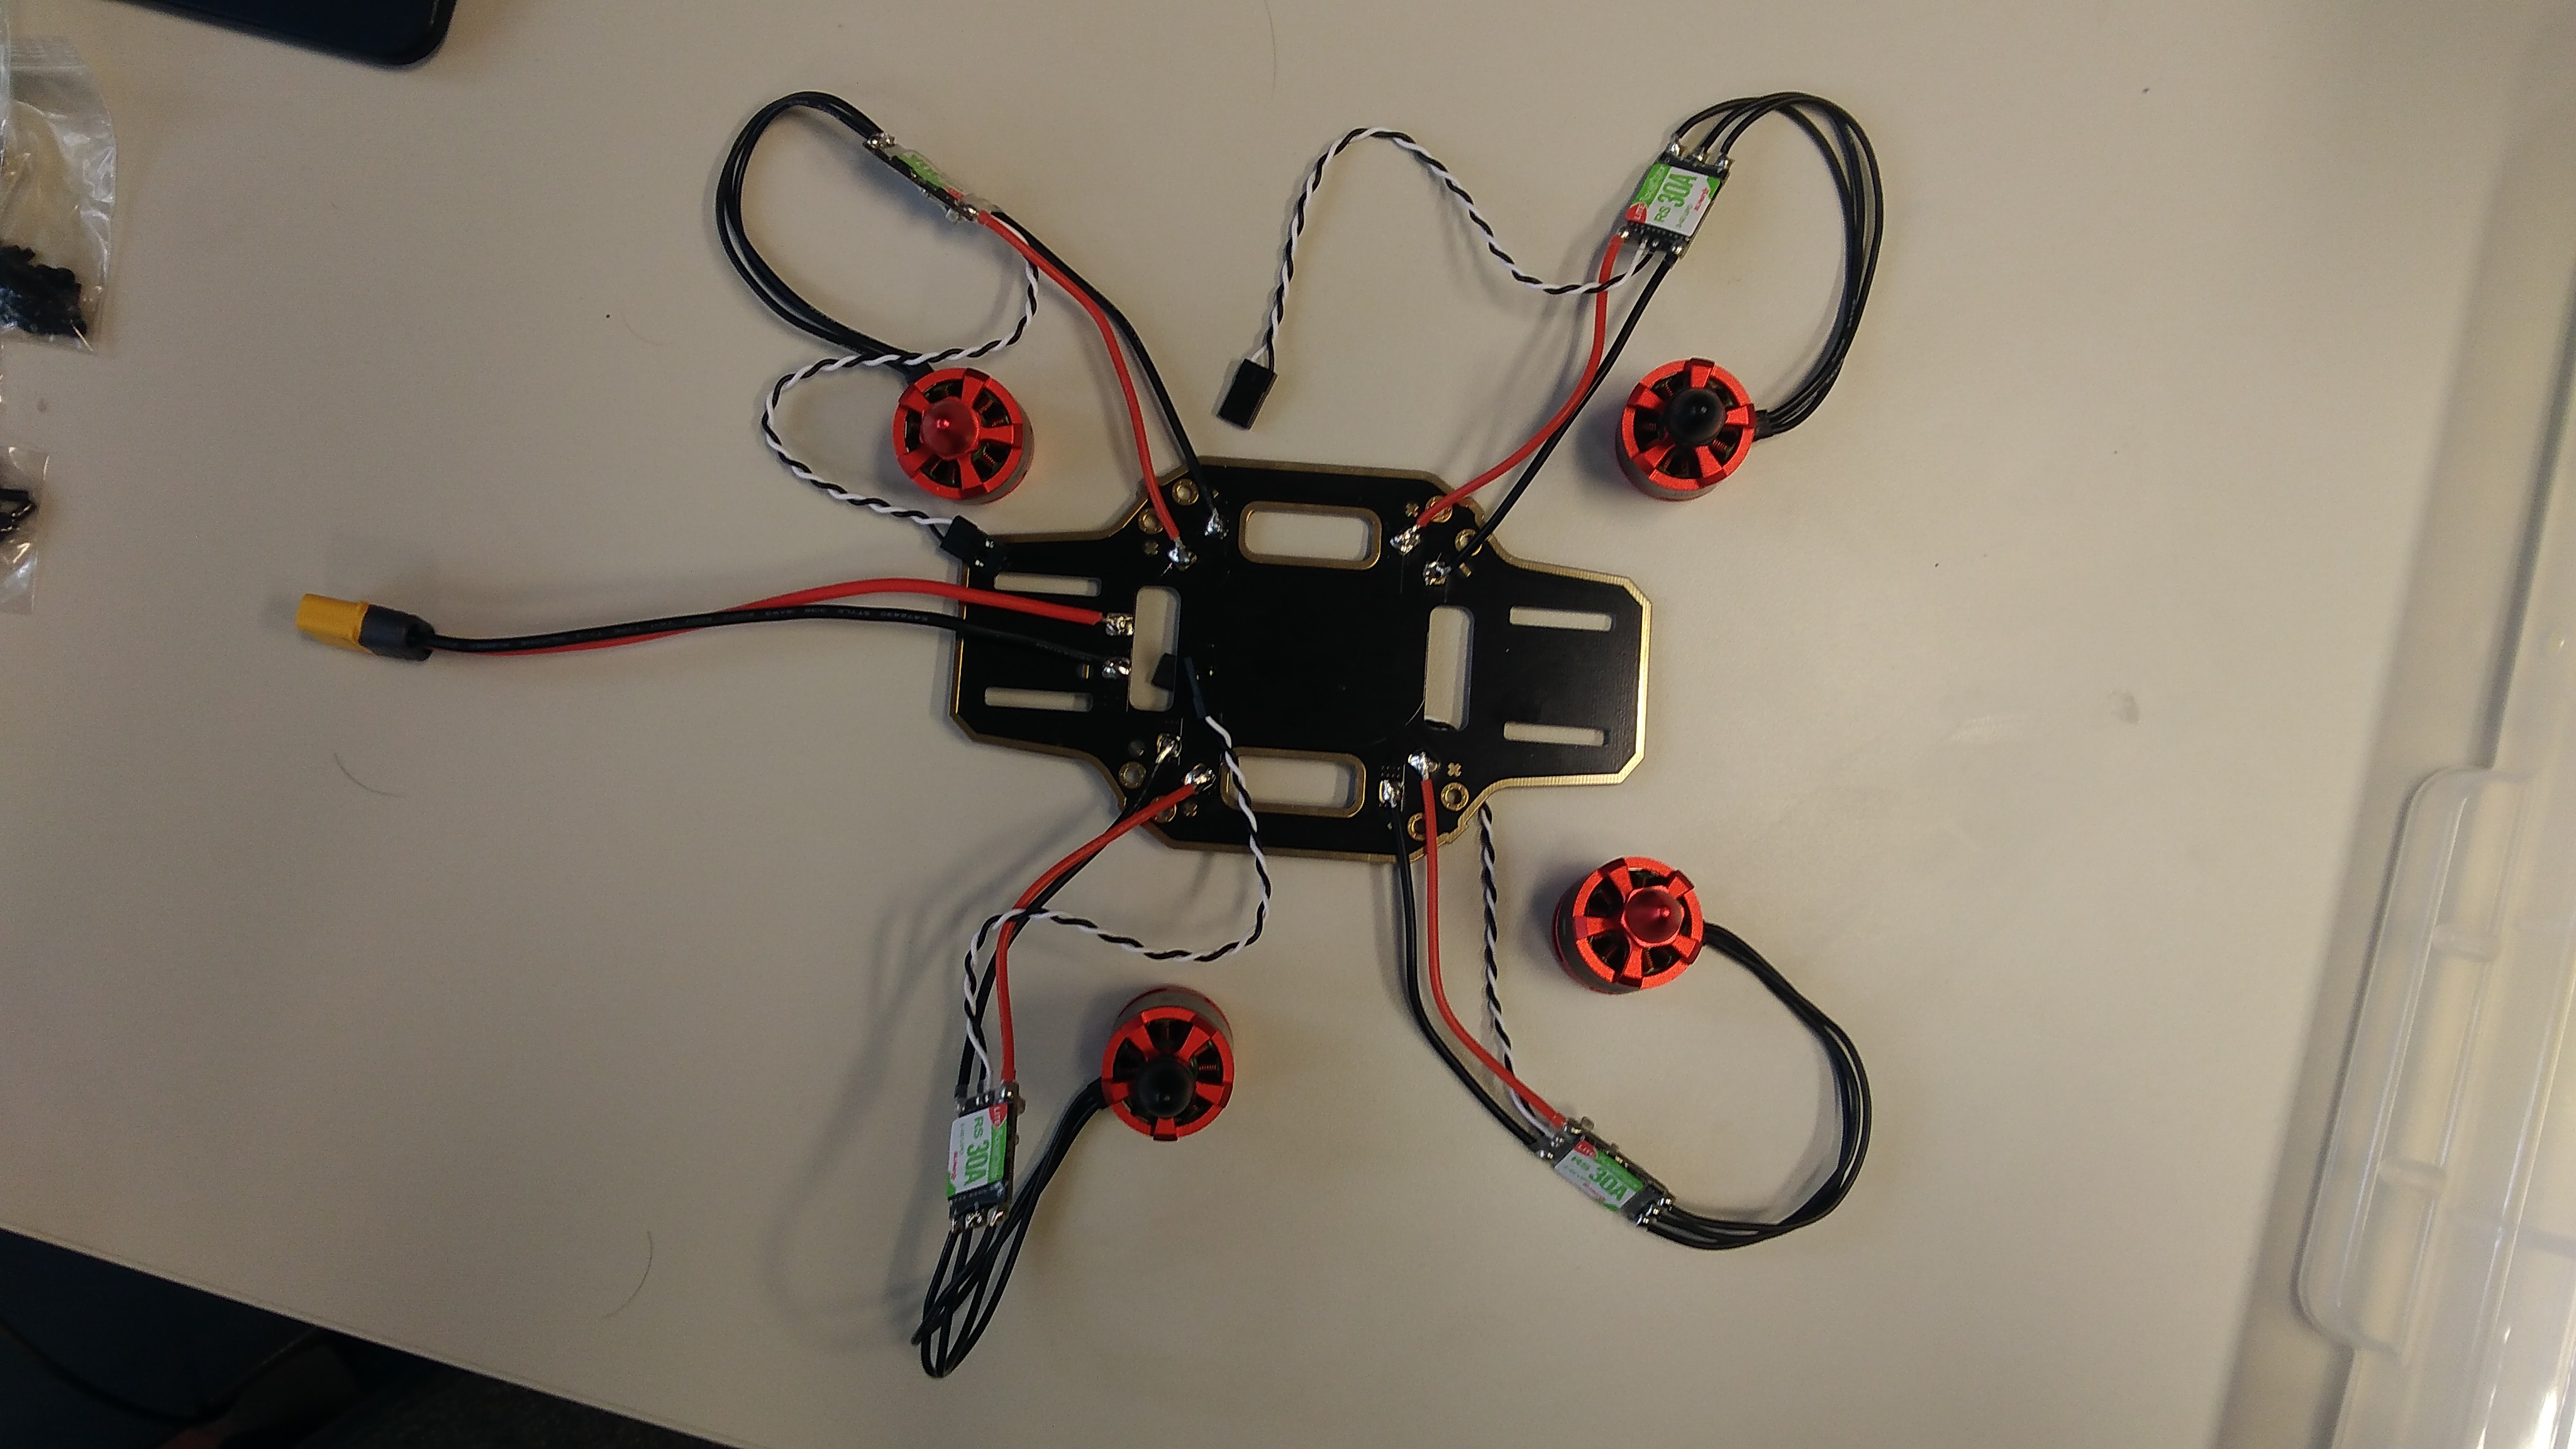
\includegraphics[width=\textwidth]{building/pdb_done.jpg}
        \caption{Done}
        \label{fig:pdb_done}
    \end{subfigure}
    \caption{Soldering}\label{fig:soldering}
\end{figure}


\section{Arms}
To attach the arm to the PDB, you will need:
\begin{itemize}
    \item the previous assembly,
    \item the frame Kit,
    \item the 4 arms
    \item 8 M2 screws.
\end{itemize}
The sequence of steps that have to be followed are:
\begin{enumerate}
    \item Place the esc cable in between the arm fixations.
    \item Screw the arm to the PDB, but not too tight to be able to adjust the arm position later.
\end{enumerate}

\begin{figure}[!ht]
    \centering
    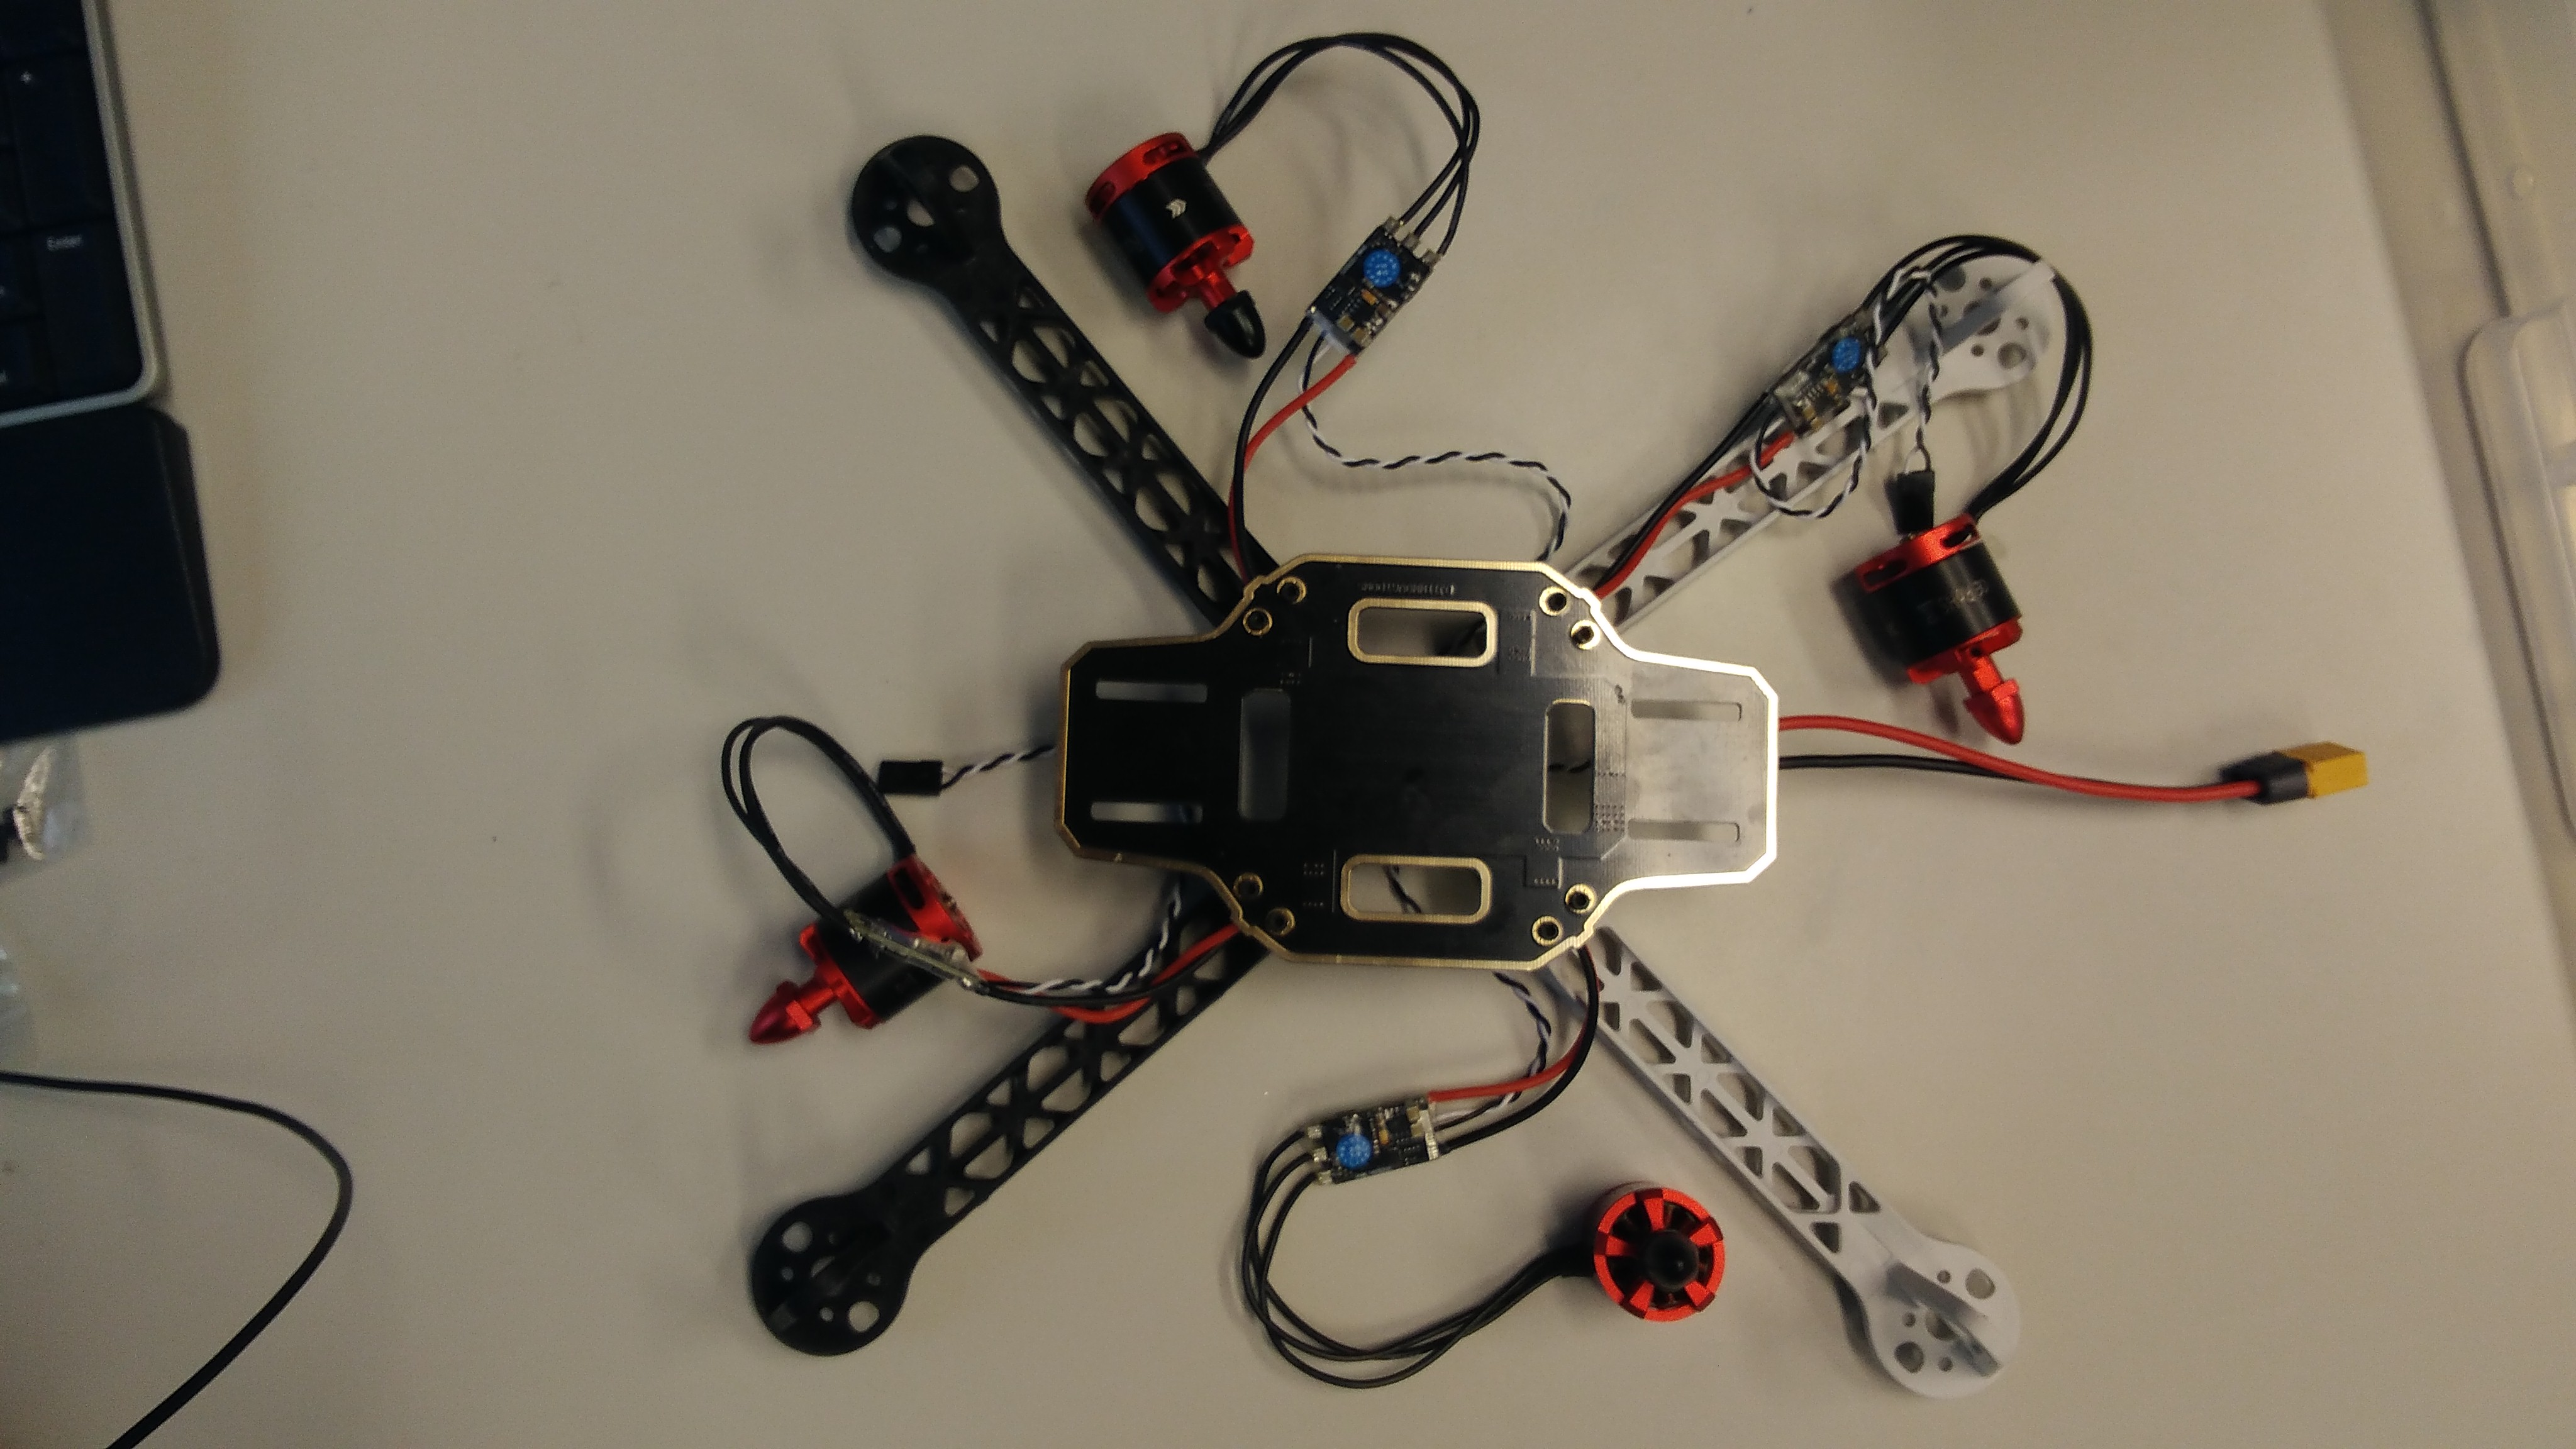
\includegraphics[width=0.5\textwidth]{building/attaching_arms.jpg}
    \caption{Attaching arms}
    \label{fig:arms}
\end{figure}




\section{Motors}
To attach the motors to the frame, you will need:
\begin{itemize}
    \item The previous assembly,
    \item the frame Kit with 16 M3 screw.
\end{itemize}
The sequence of steps that have to be followed are:
\begin{enumerate}
    \item Check where each motor should be placed by looking how they should rotate (clockwise or counterclockwise).
    \item Screw the motors to the frame.
\end{enumerate}

{\color{blue} Add picture of one motor fixation up close}
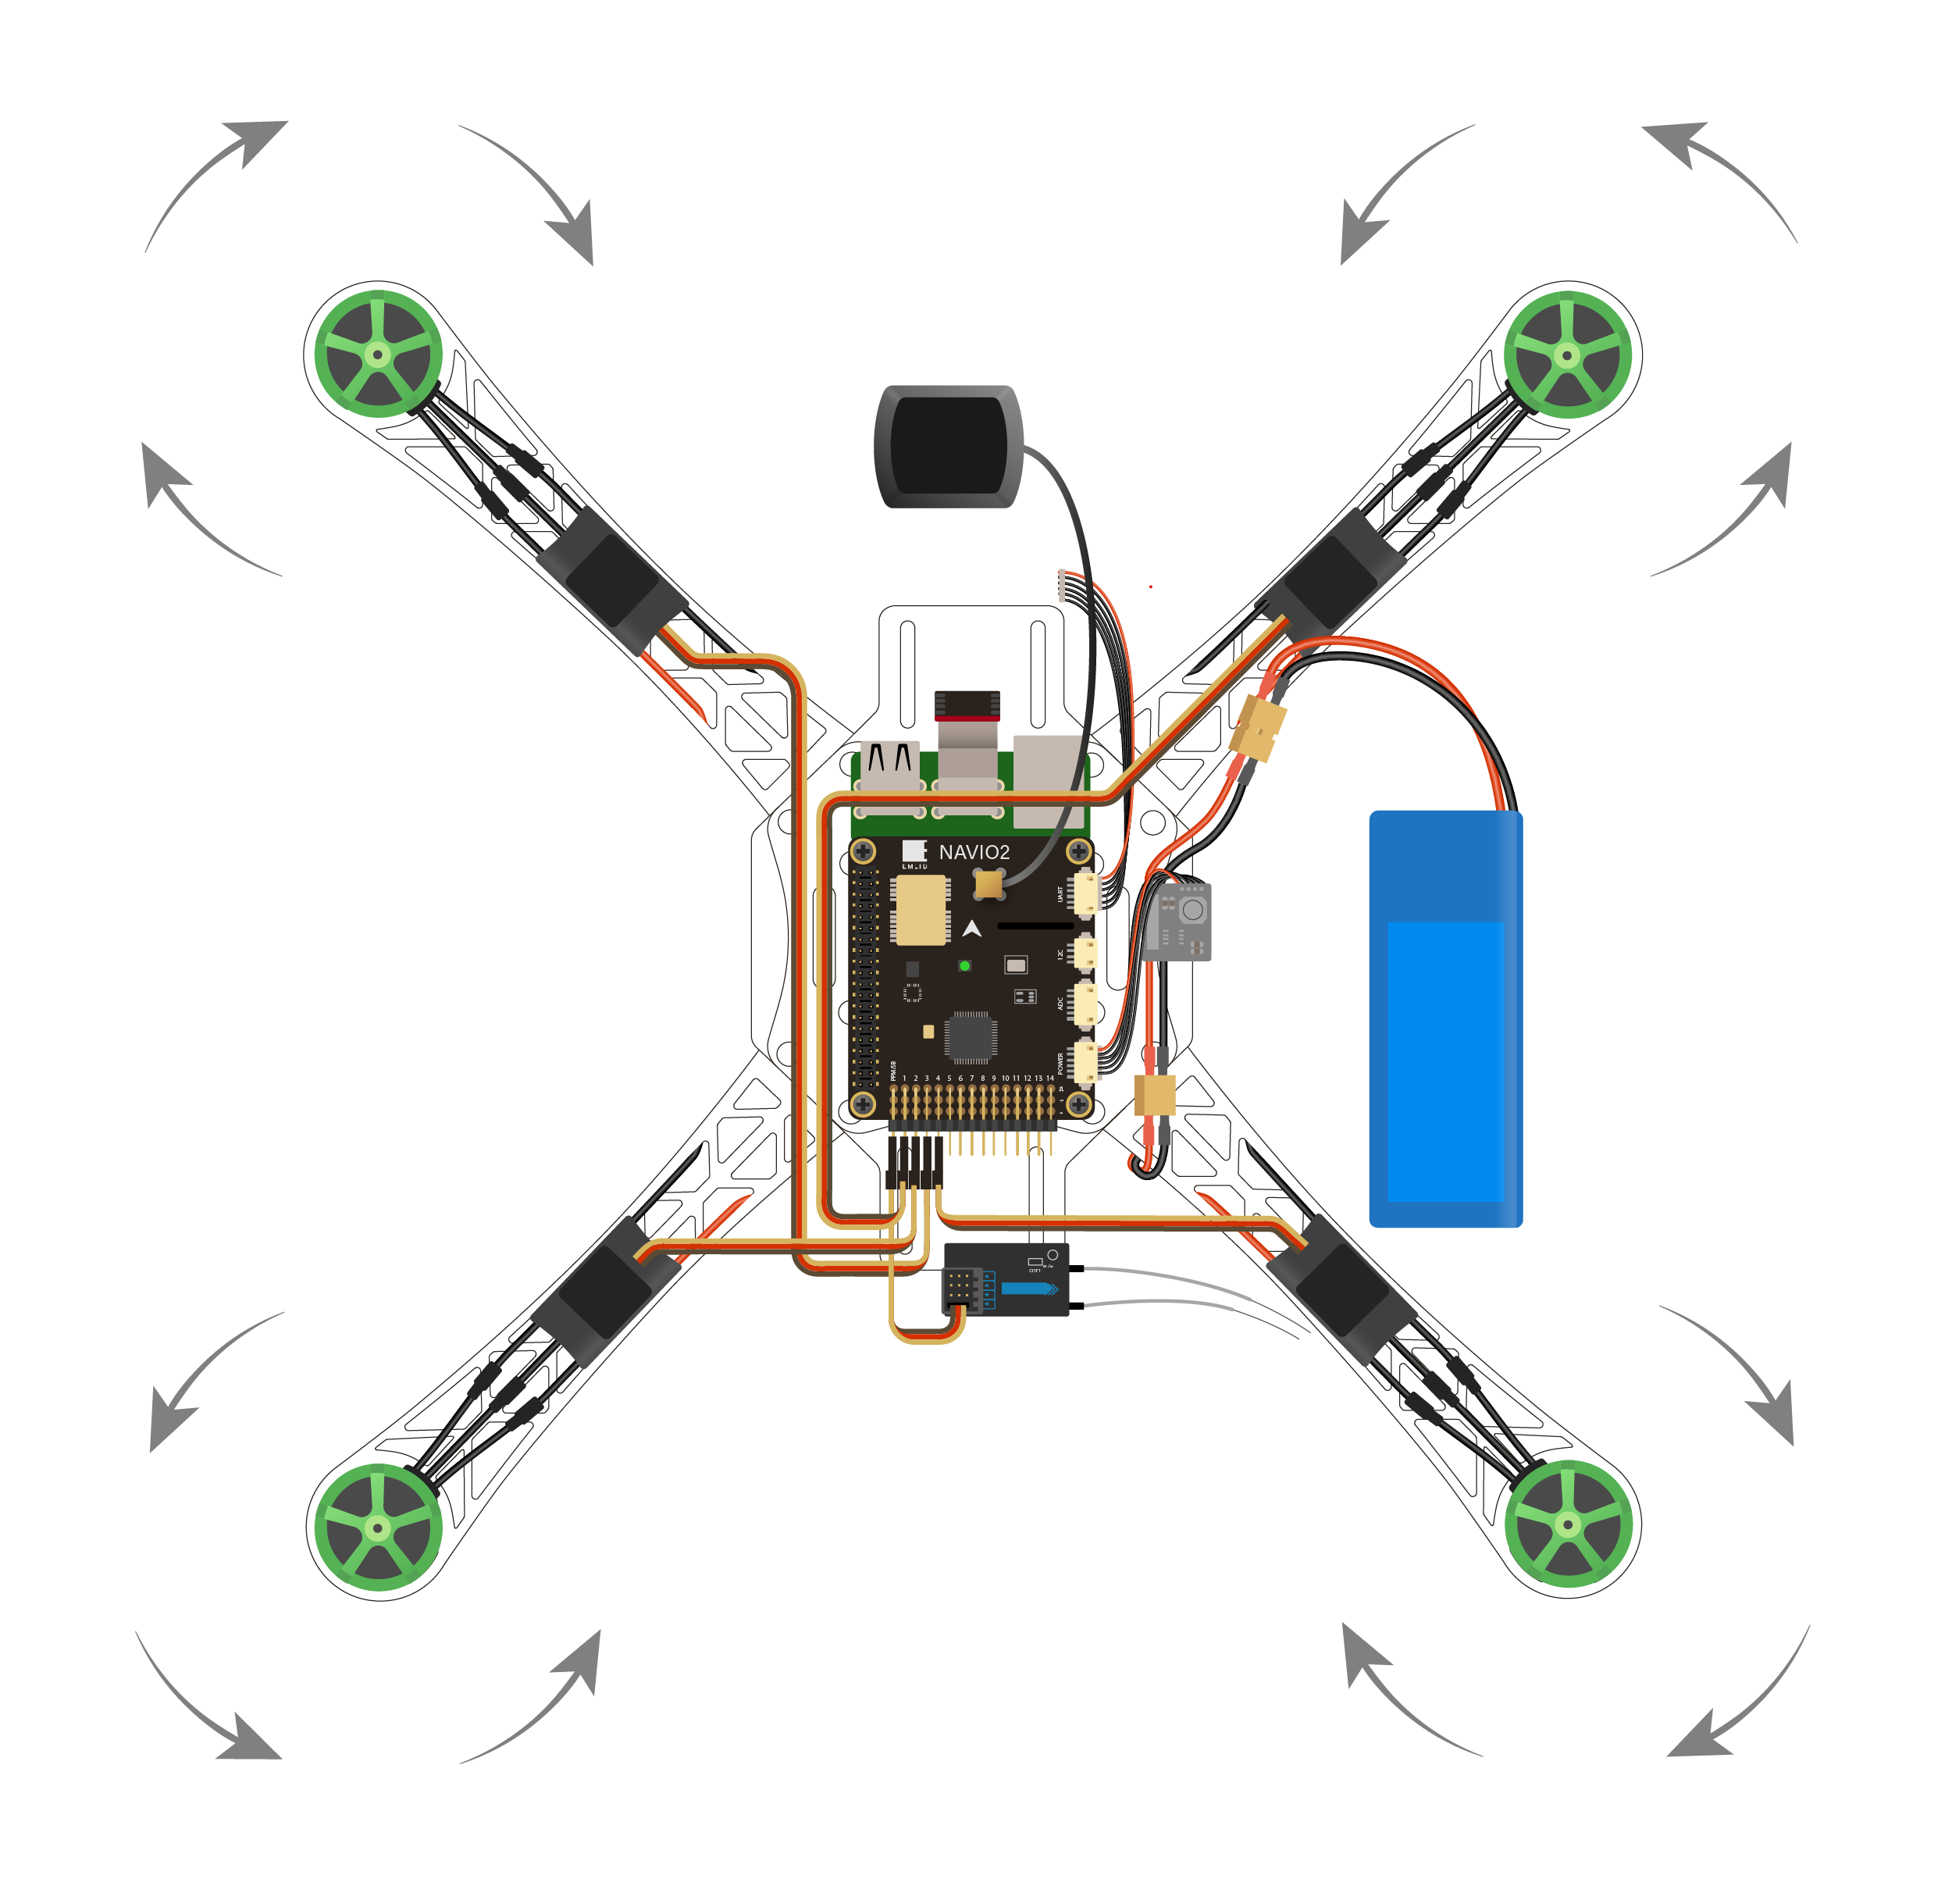
\includegraphics[width=.4\linewidth]{building/navio2_typical_quadcopter_setup_frame.png}

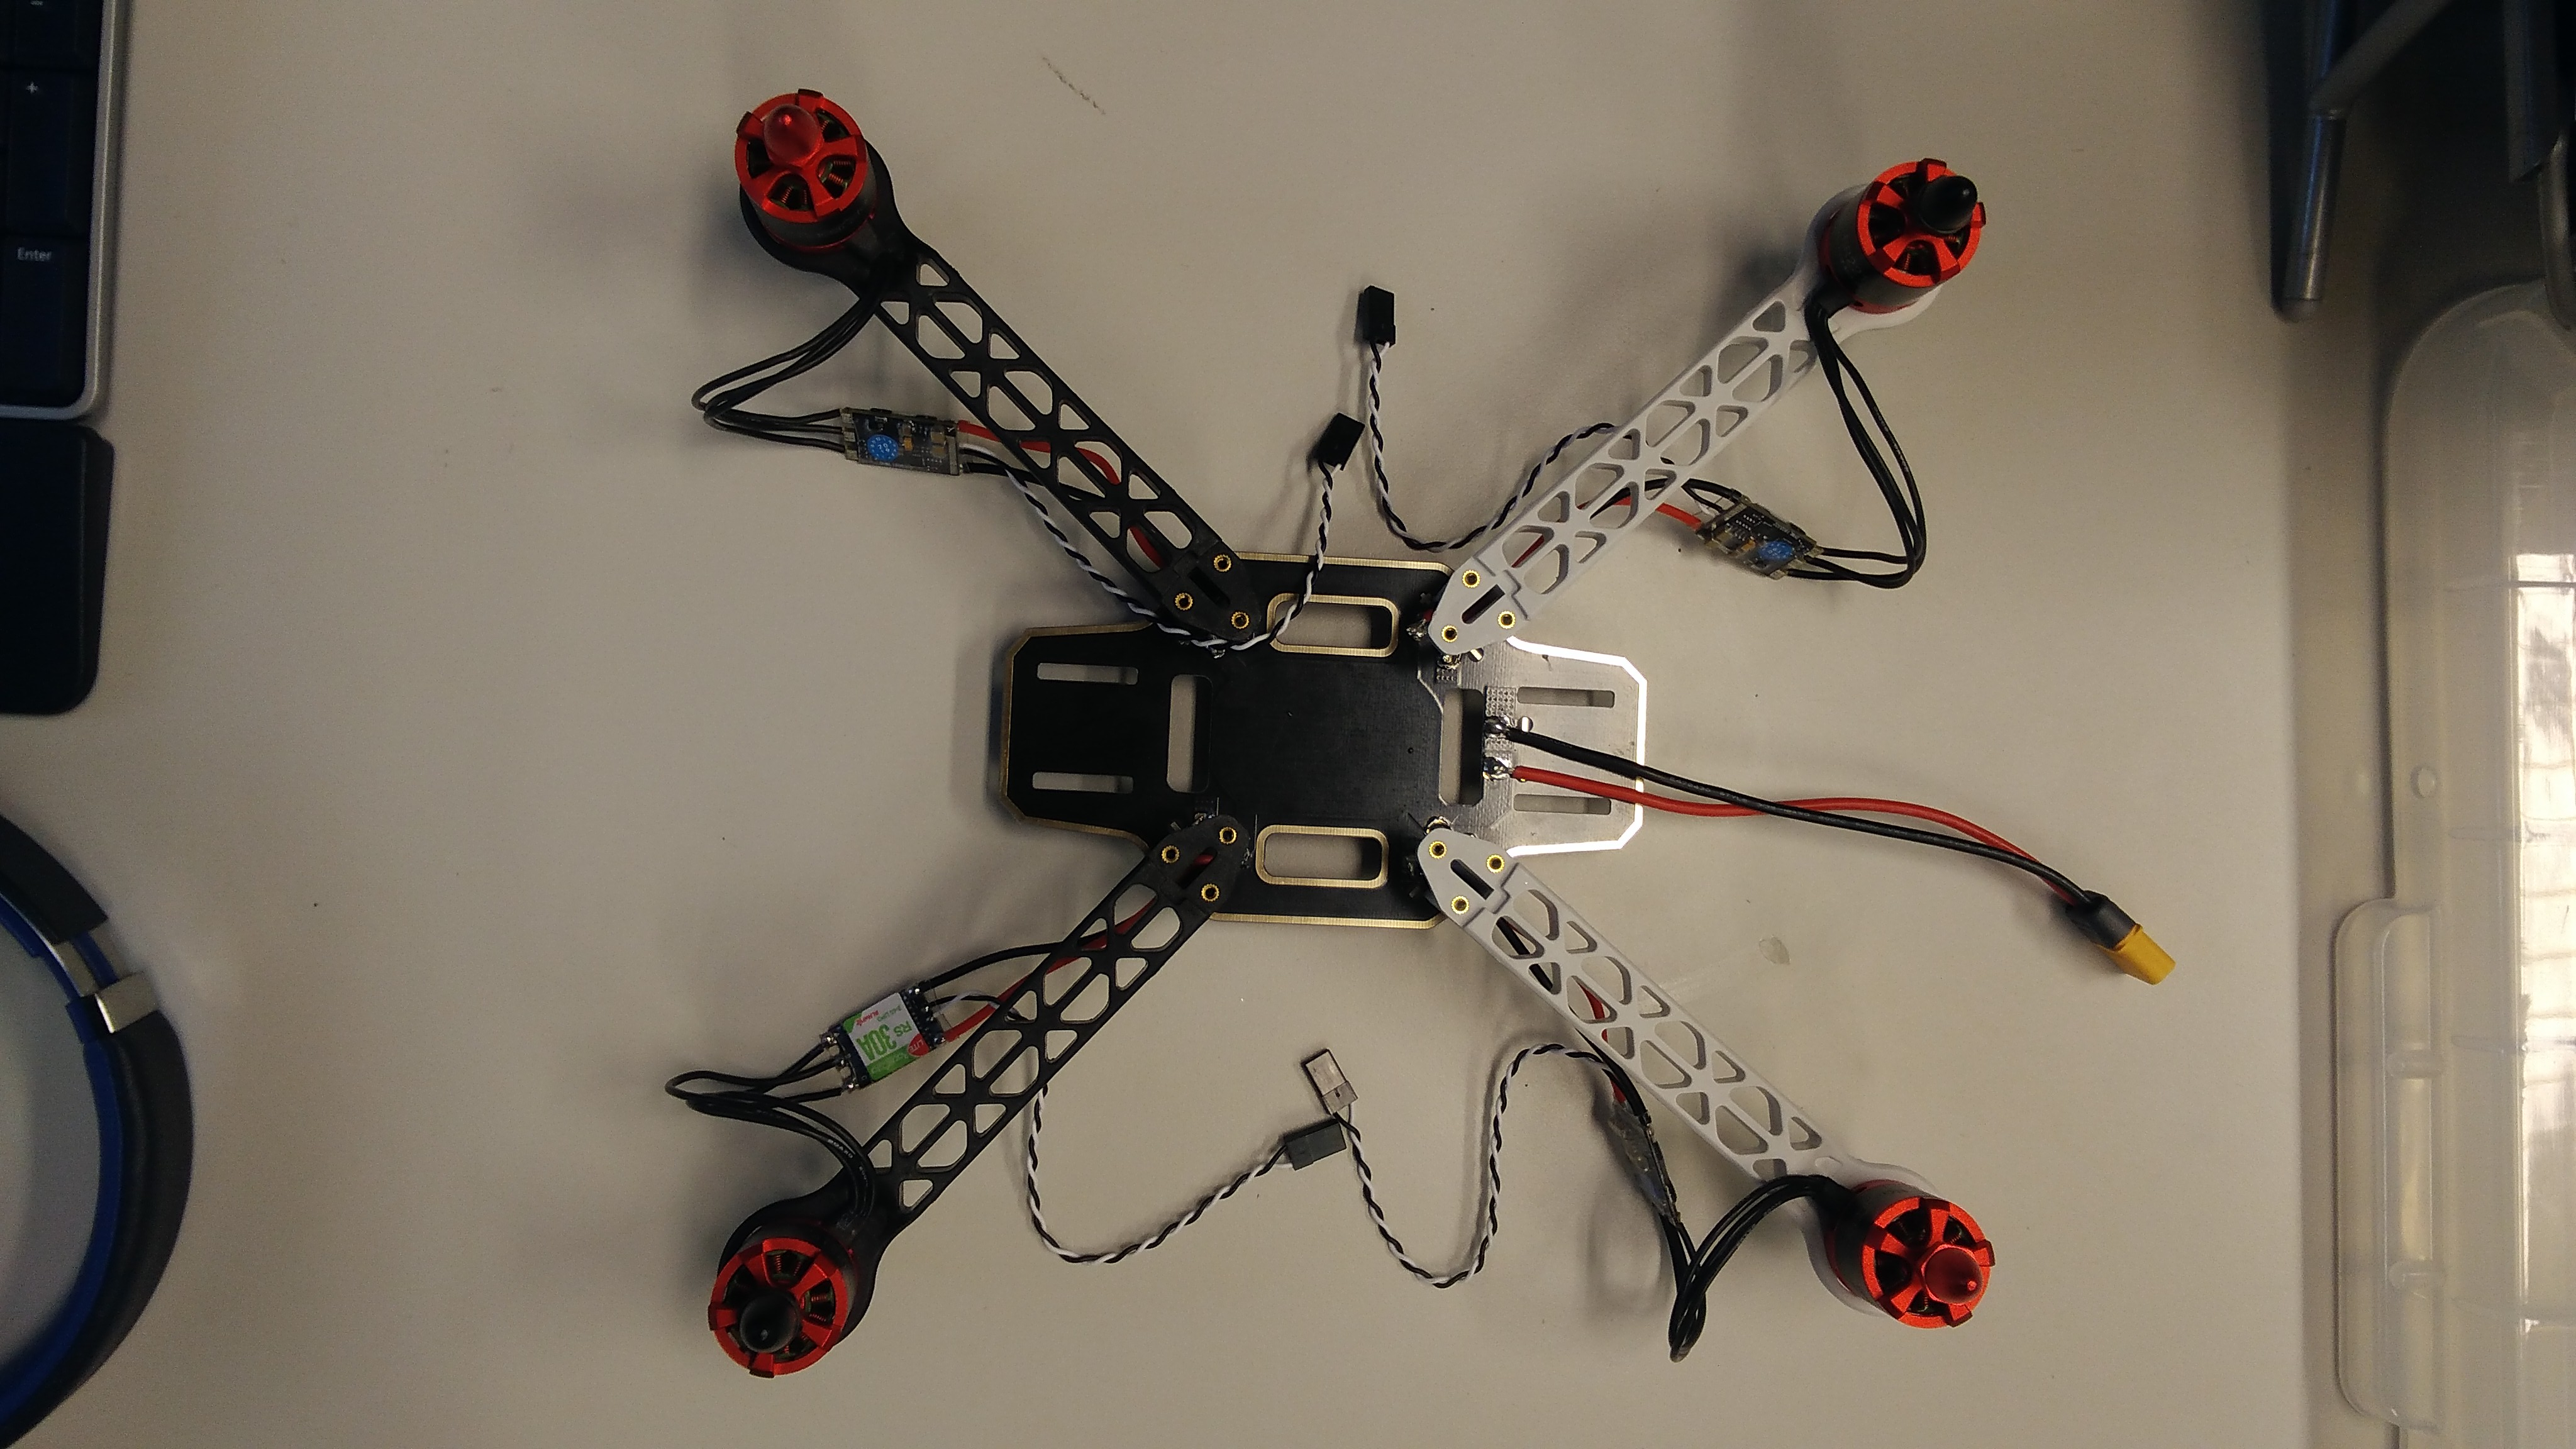
\includegraphics[width=.4\linewidth]{building/installing_motors_up.jpg}
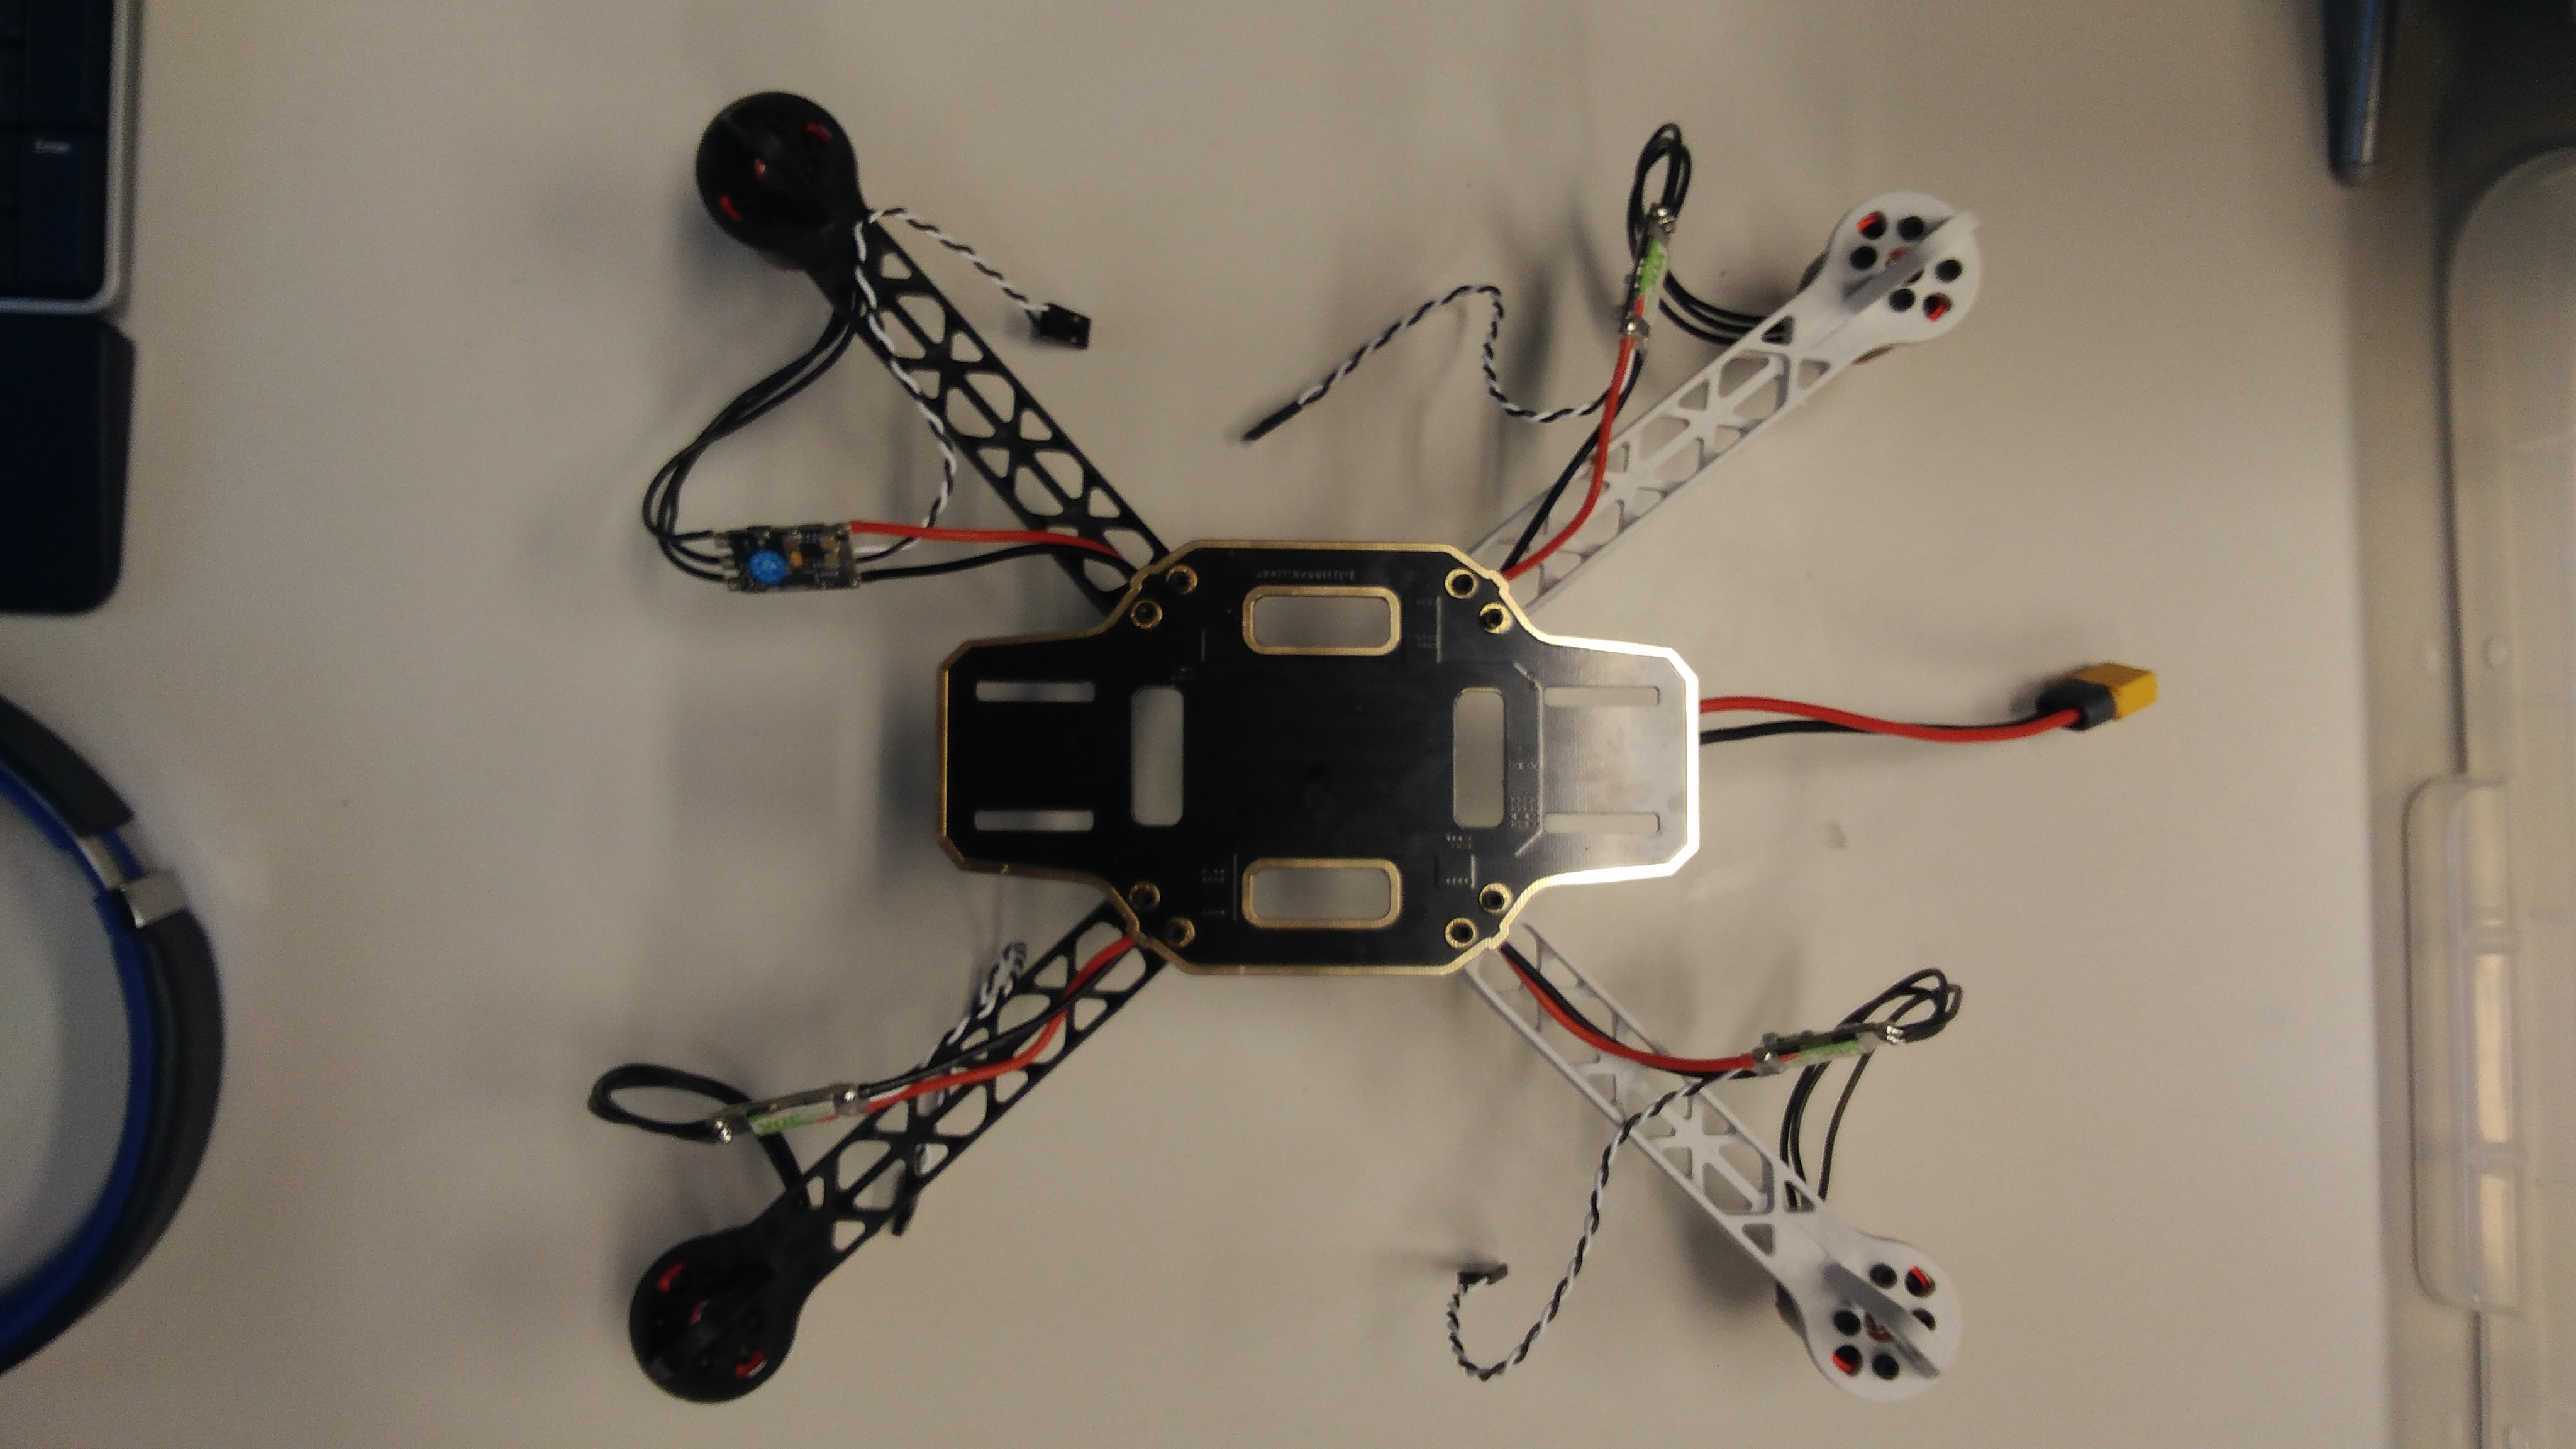
\includegraphics[width=.4\linewidth]{building/installing_motors_down.jpg}

\section{Raspberry Pi and Navio2}
\subsection{Attaching the Navio2 to a Raspberry Pi}
It is advised to follow this official tutorial \cite{emlid_hardware_setup}.

\subsection{Attaching the Raspberry Pi to the frame}
To attach the Raspberry Pi to the frame, you will need:
\begin{itemize}
    \item the previous assembly,
    \item the frame Kit
    \item the top plate
    \item 12 M2 screws,
    \item straps,
    \item insulation tape
\end{itemize}
Note that the side with the usb port on the raspberry pie and the arrow on the navio2 represent the front of the drone.\\
The sequence of steps that have to be followed are:
\begin{enumerate}
    \item Add insulation tape under the raspberry pie.
    \item Screw the top plate to the rest. You can now tighten all the screws.
    \item Strap the Raspberry to the top plate.
\end{enumerate}

This is not the best solution, it does not evacuate the heat well. Creating a 3D support with damped spacer could address this problem and reduce the vibration of the Raspberry Pi. Or try a solution with double sided tape.

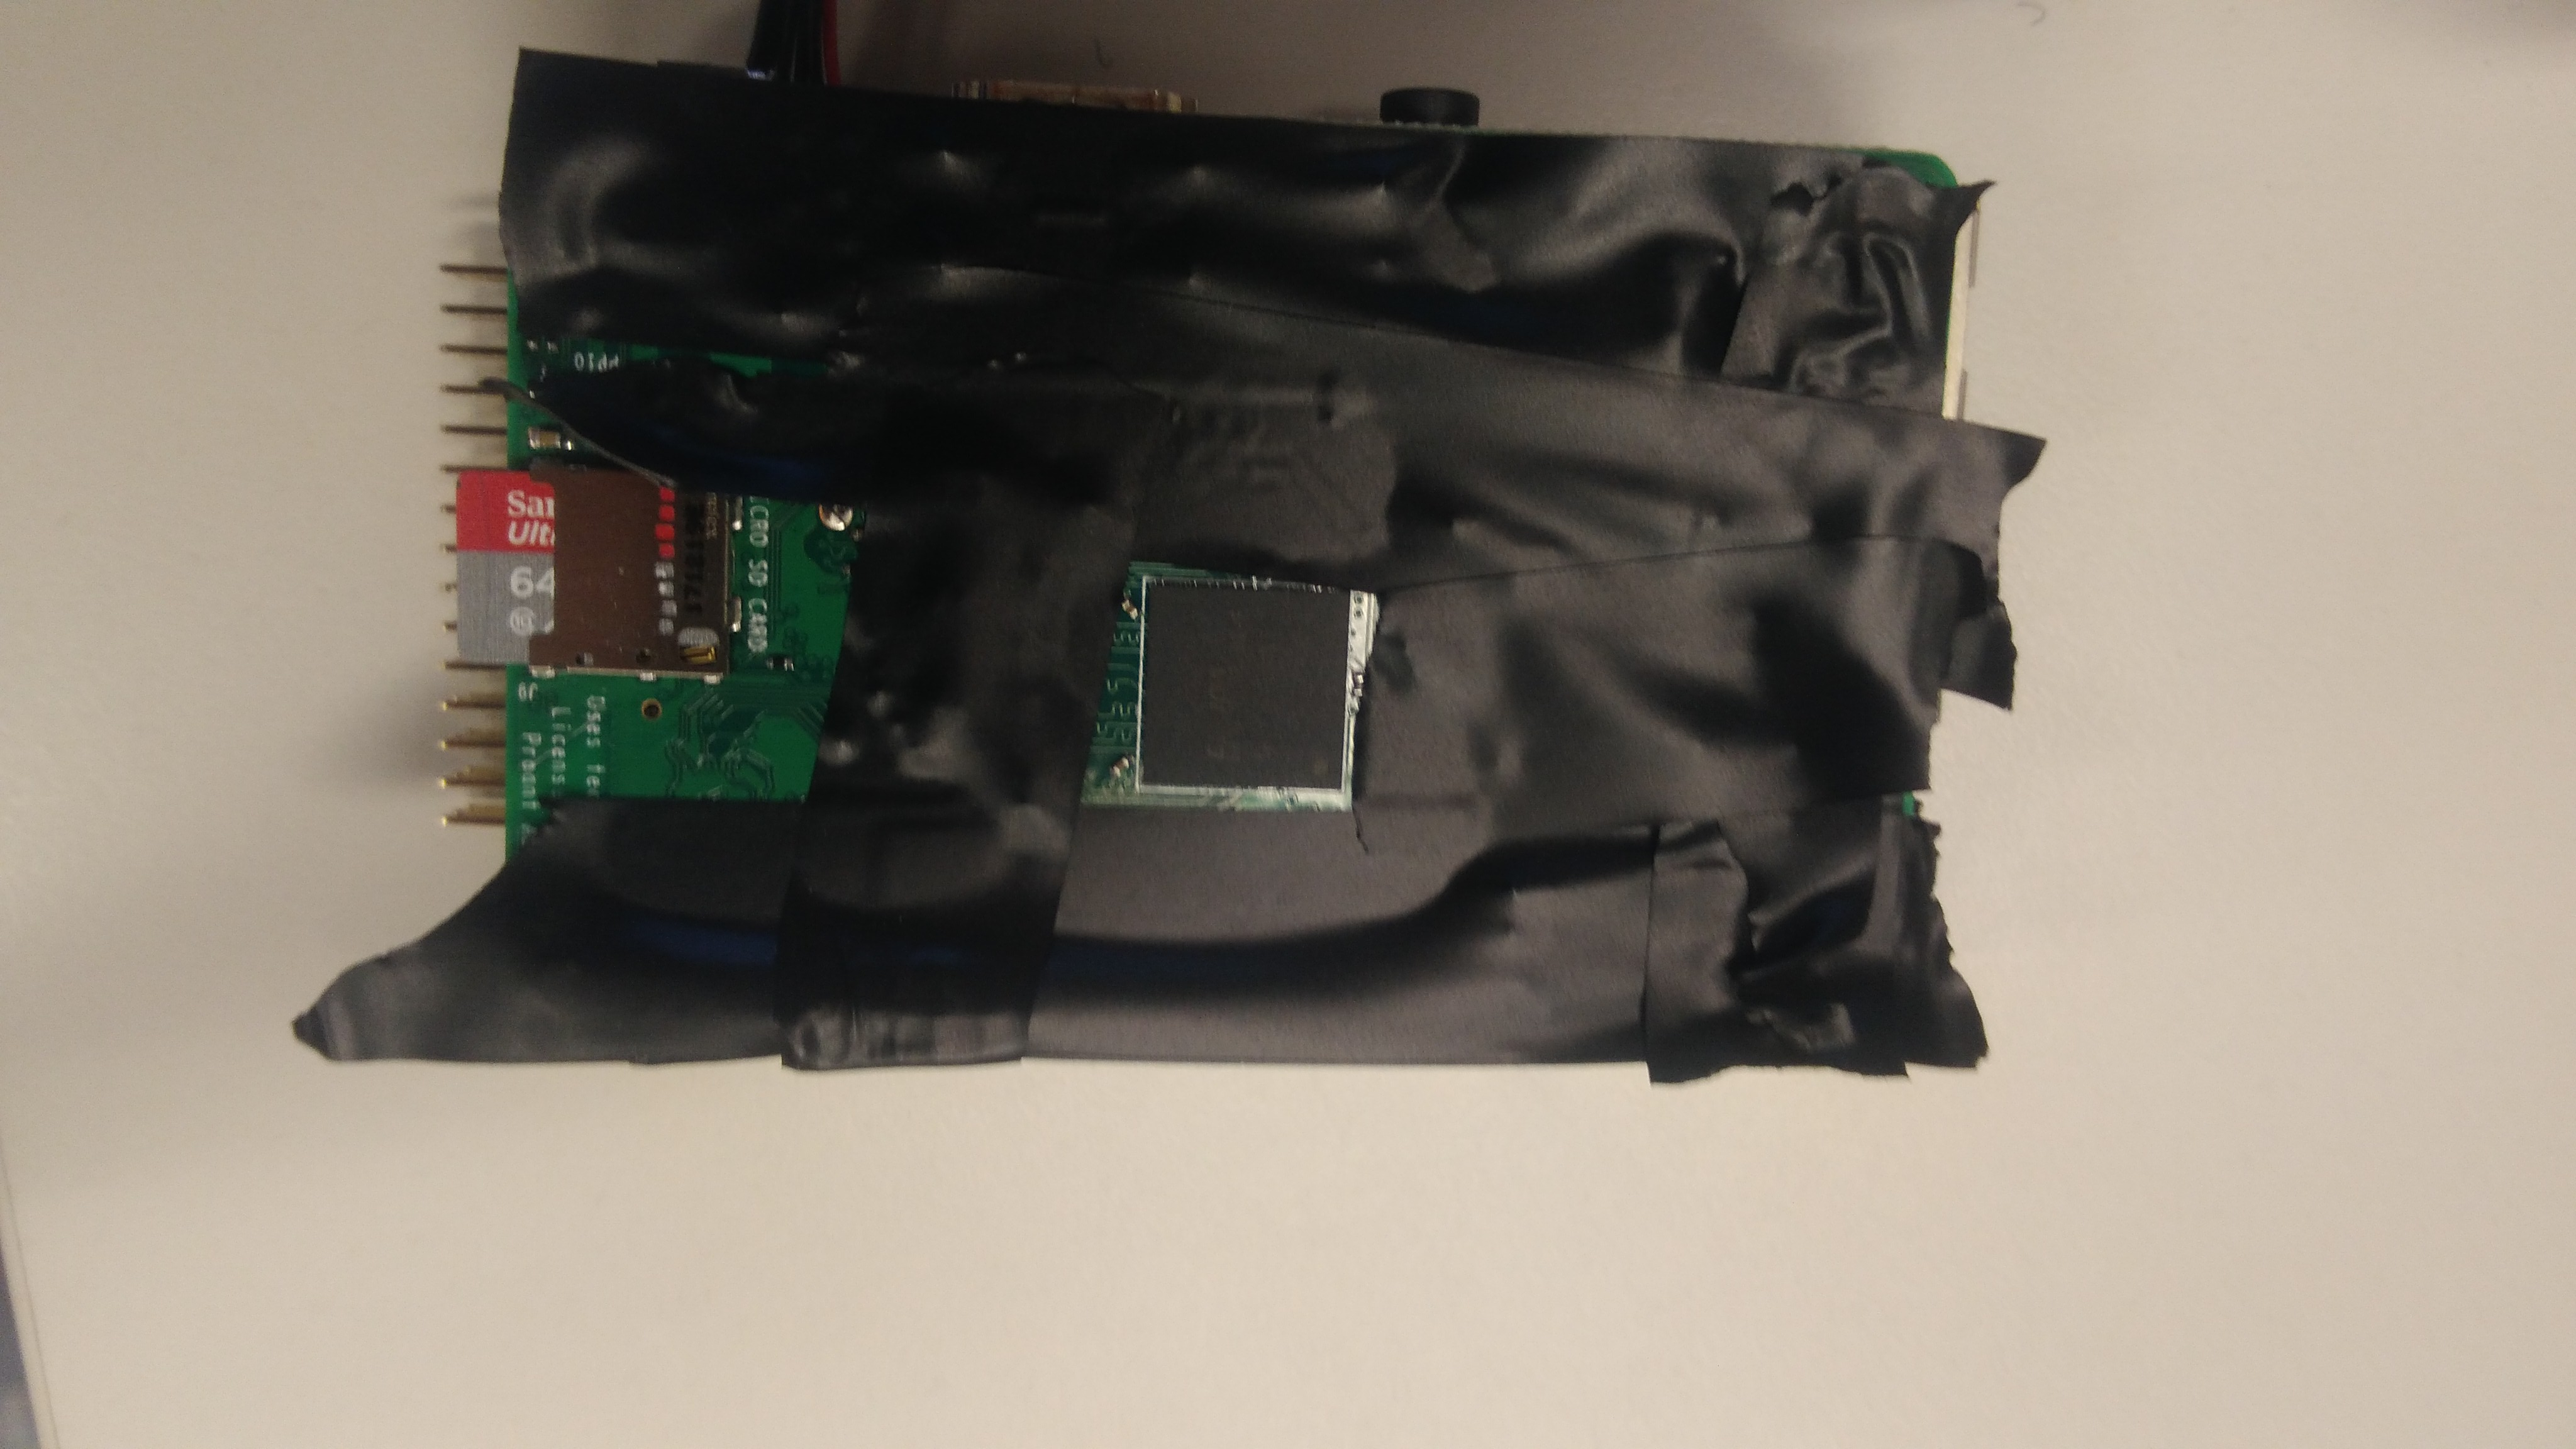
\includegraphics[width=.4\linewidth]{building/raspberry_pi_insulation.jpg}
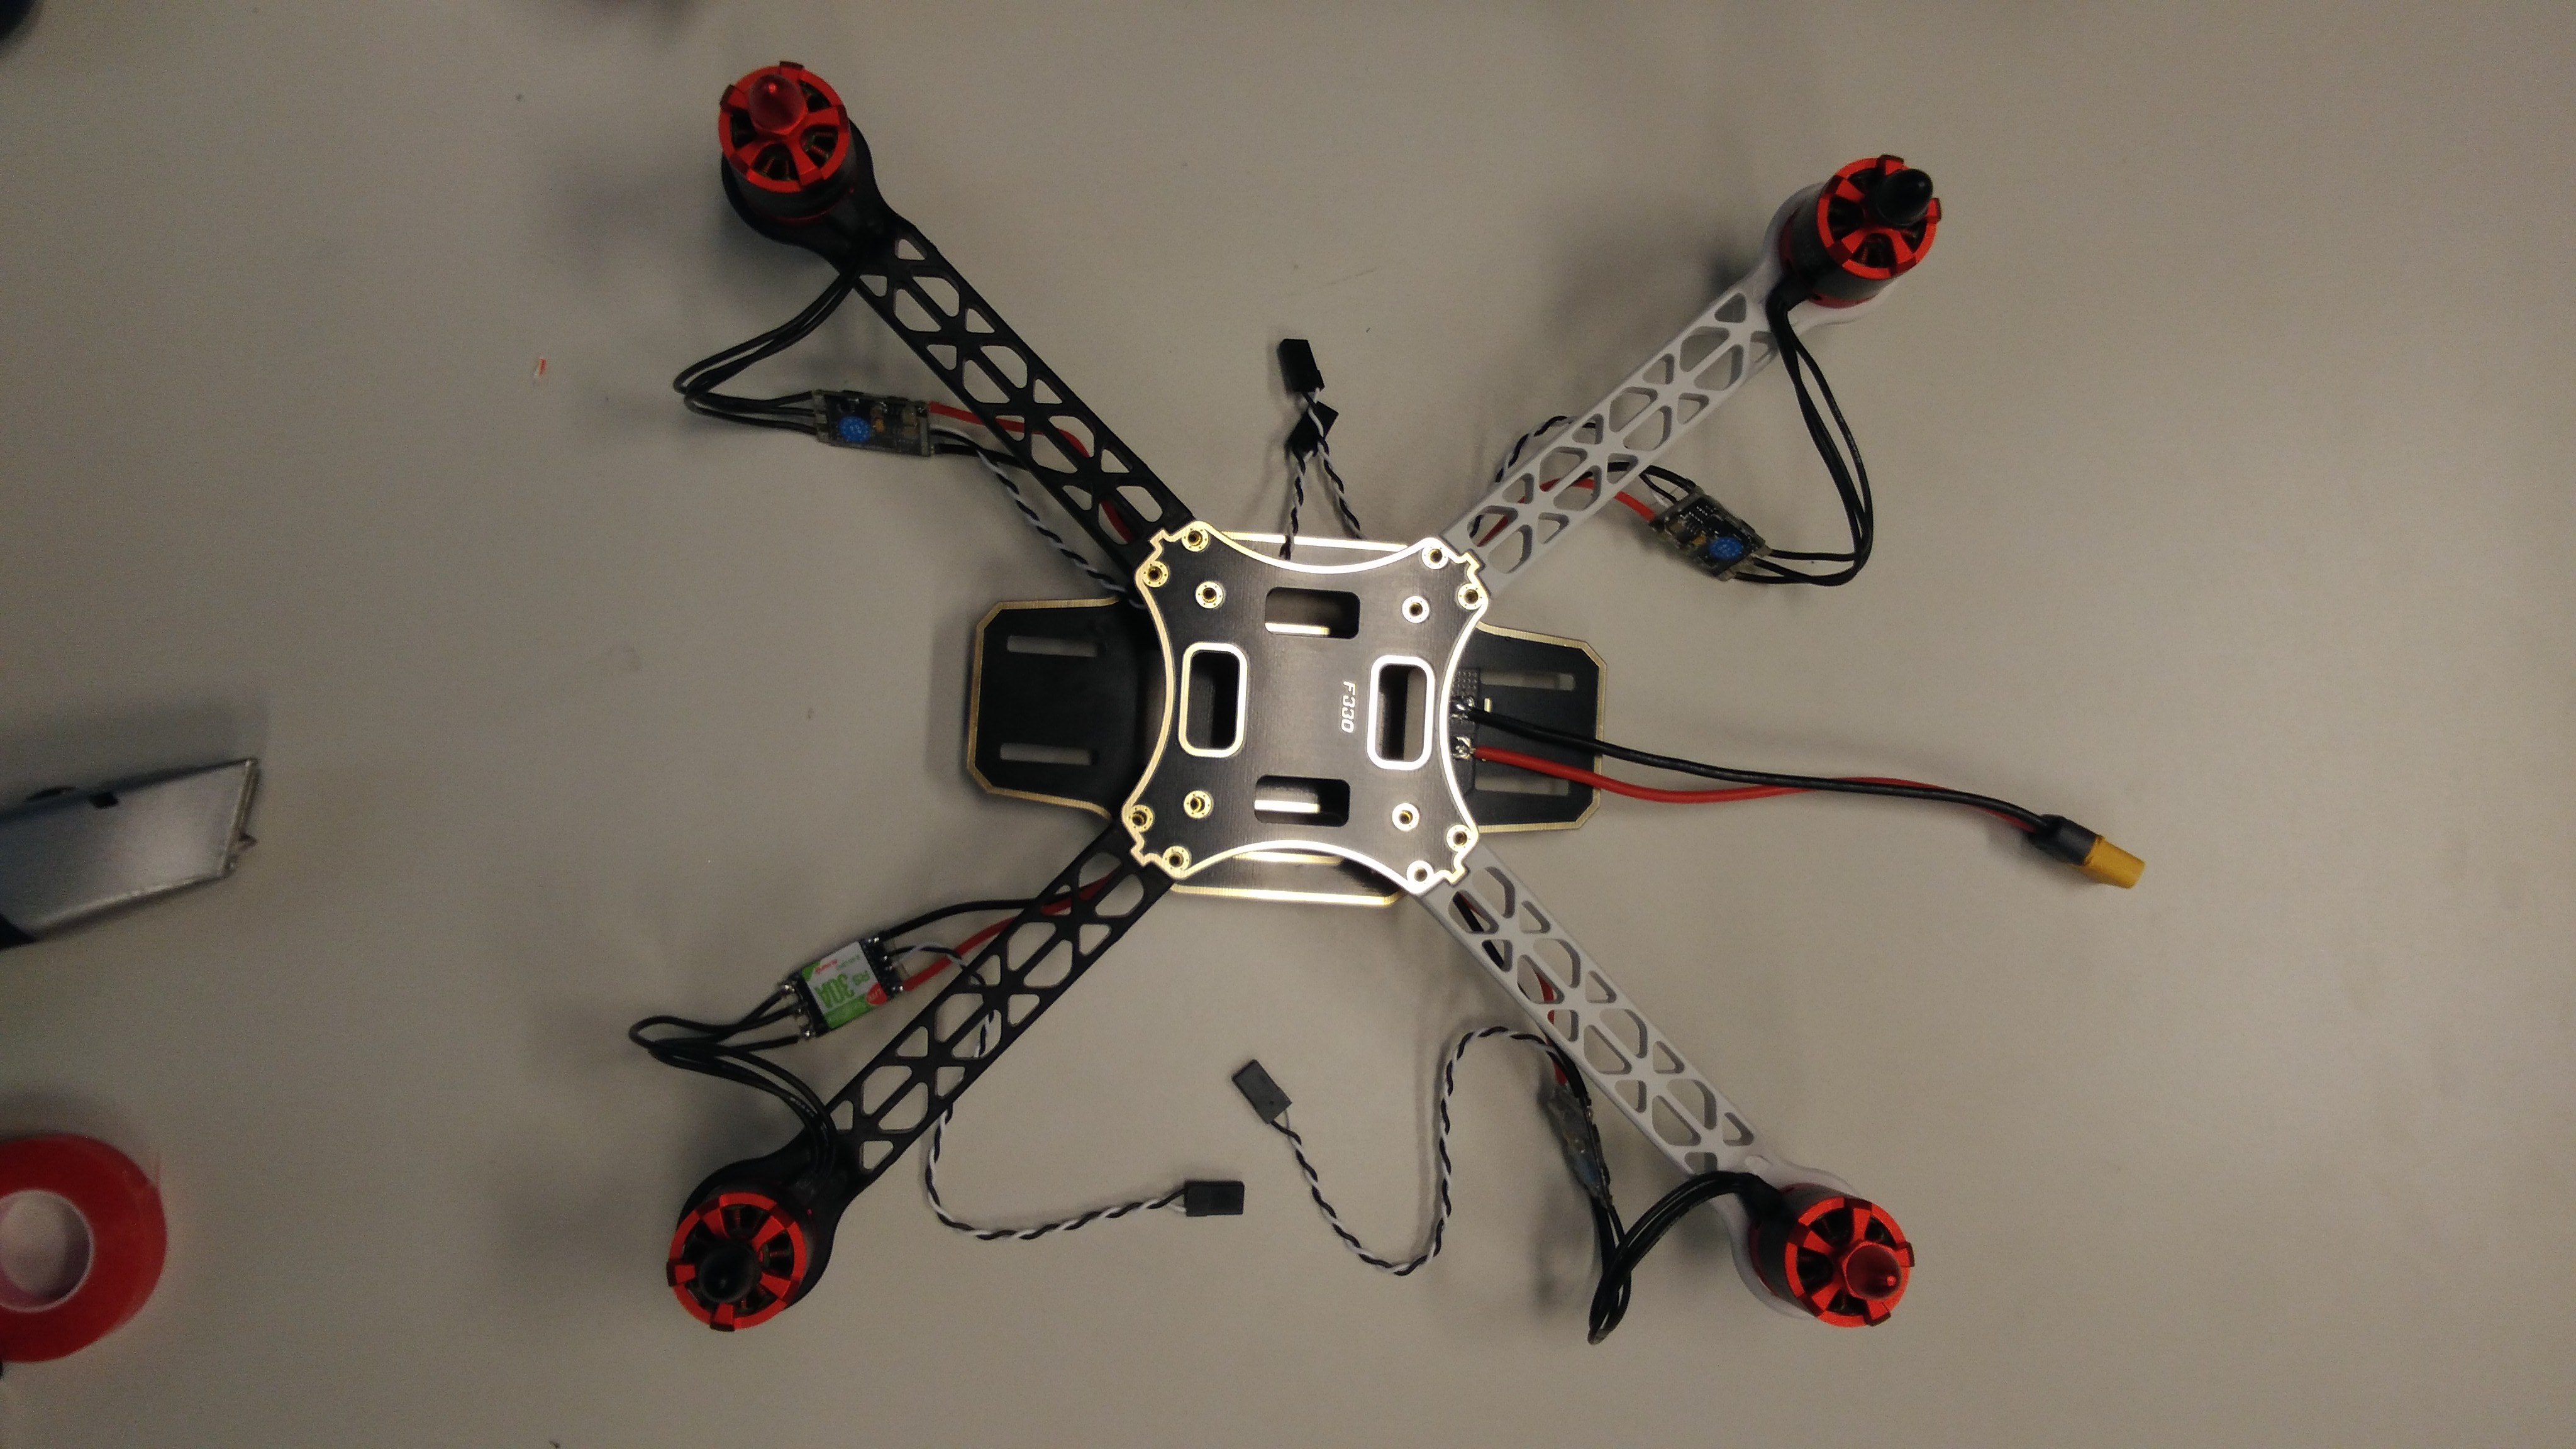
\includegraphics[width=.4\linewidth]{building/installing_top_plate.jpg}

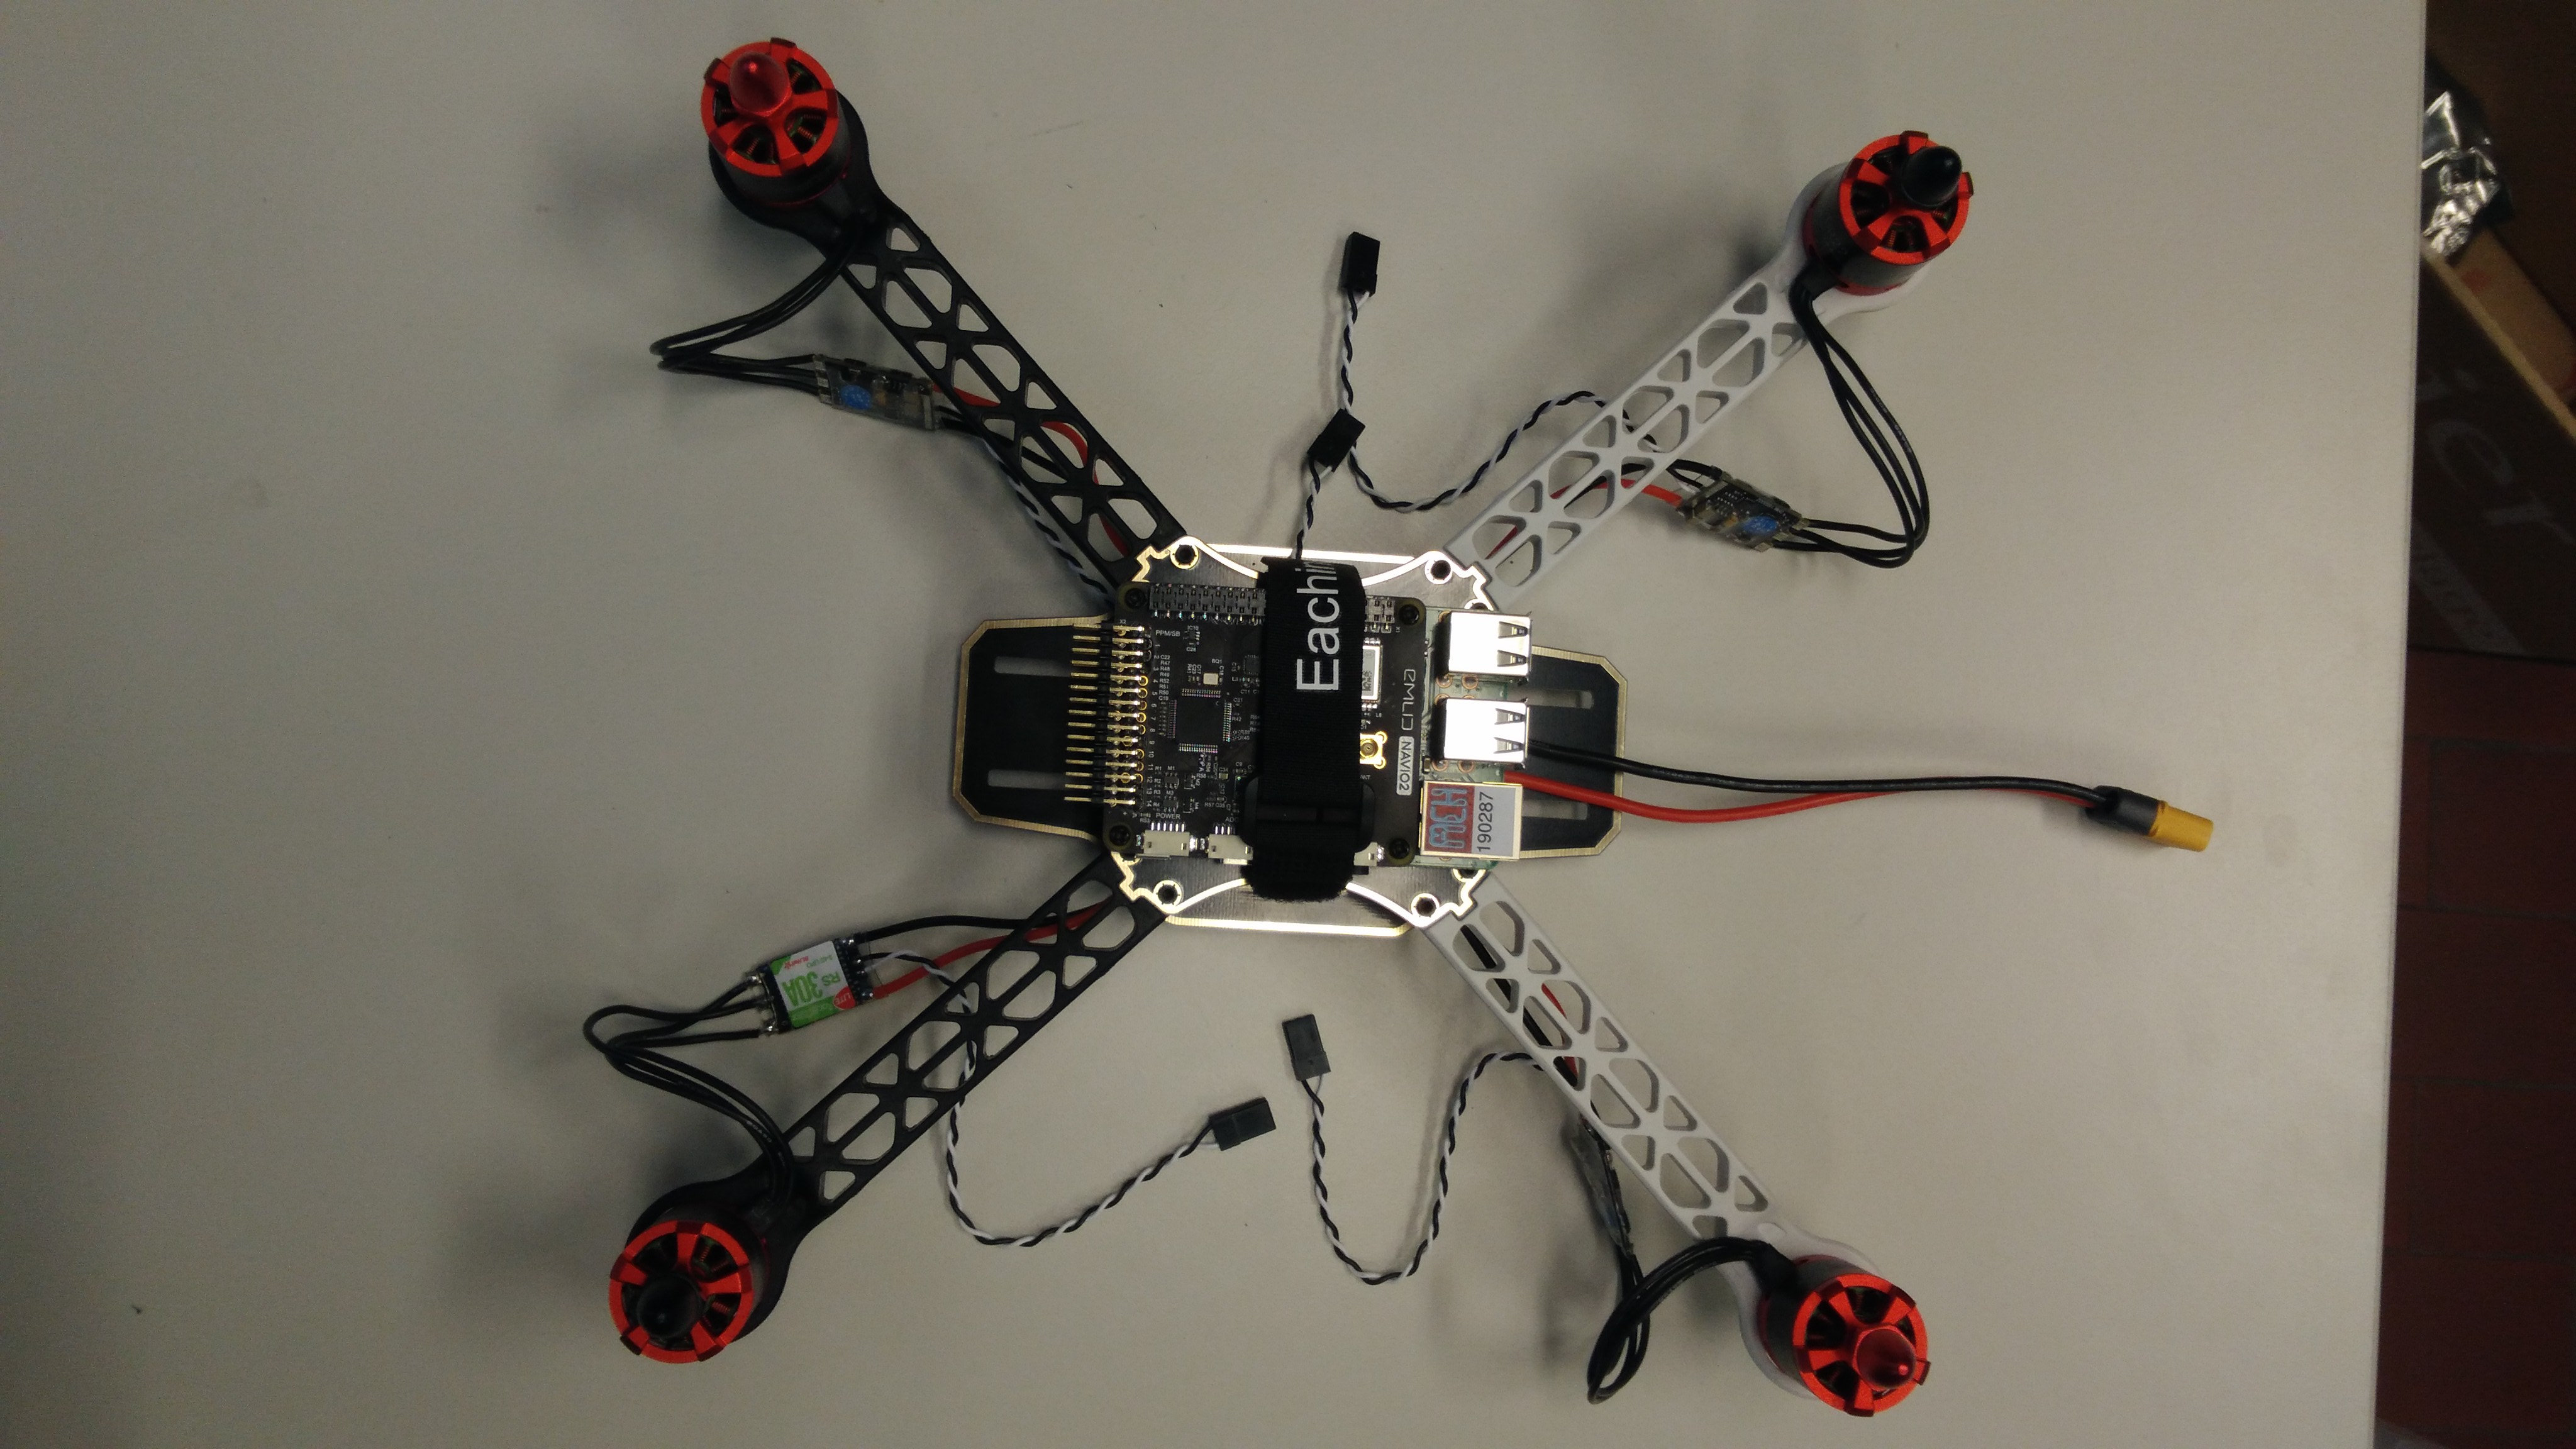
\includegraphics[width=.4\linewidth]{building/securing_raspberry_pi.jpg}

\section{Battery}
\subsection{Charging}
To charge the battery one should:
\begin{enumerate}
    \item Power the battery charger.
    \item Set the voltage to 11.1V for our drone and the current to 1A for charging.
    \item Place the battery in the fire proof bag. This is absolutely require as a safety issue since LiPo batteries can catch fire.
    \item Connect the battery to the charger. For the main lead beware of the polarity! Red on red, black on black. For the balance lead connect it to its appropriate place (3S).
    \item Press start until it beeps. Then press start again.
    \item It will beep when the battery is charged.
    \item You can now disconnect the battery.
\end{enumerate}
Never leave unattended a battery charging! It can catch fire if something goes wrong.
Always have a spare battery to replace the discharged one to avoid loosing time.

\subsection{Monitoring}
With the voltage battery monitor, you can check if the lipo battery is charged and it will alarm you when the voltage is too low.
{\color{orange} Explain how to connect the battery to the monitor.}
{\color{orange} Explain how to setup the voltage alarm.}
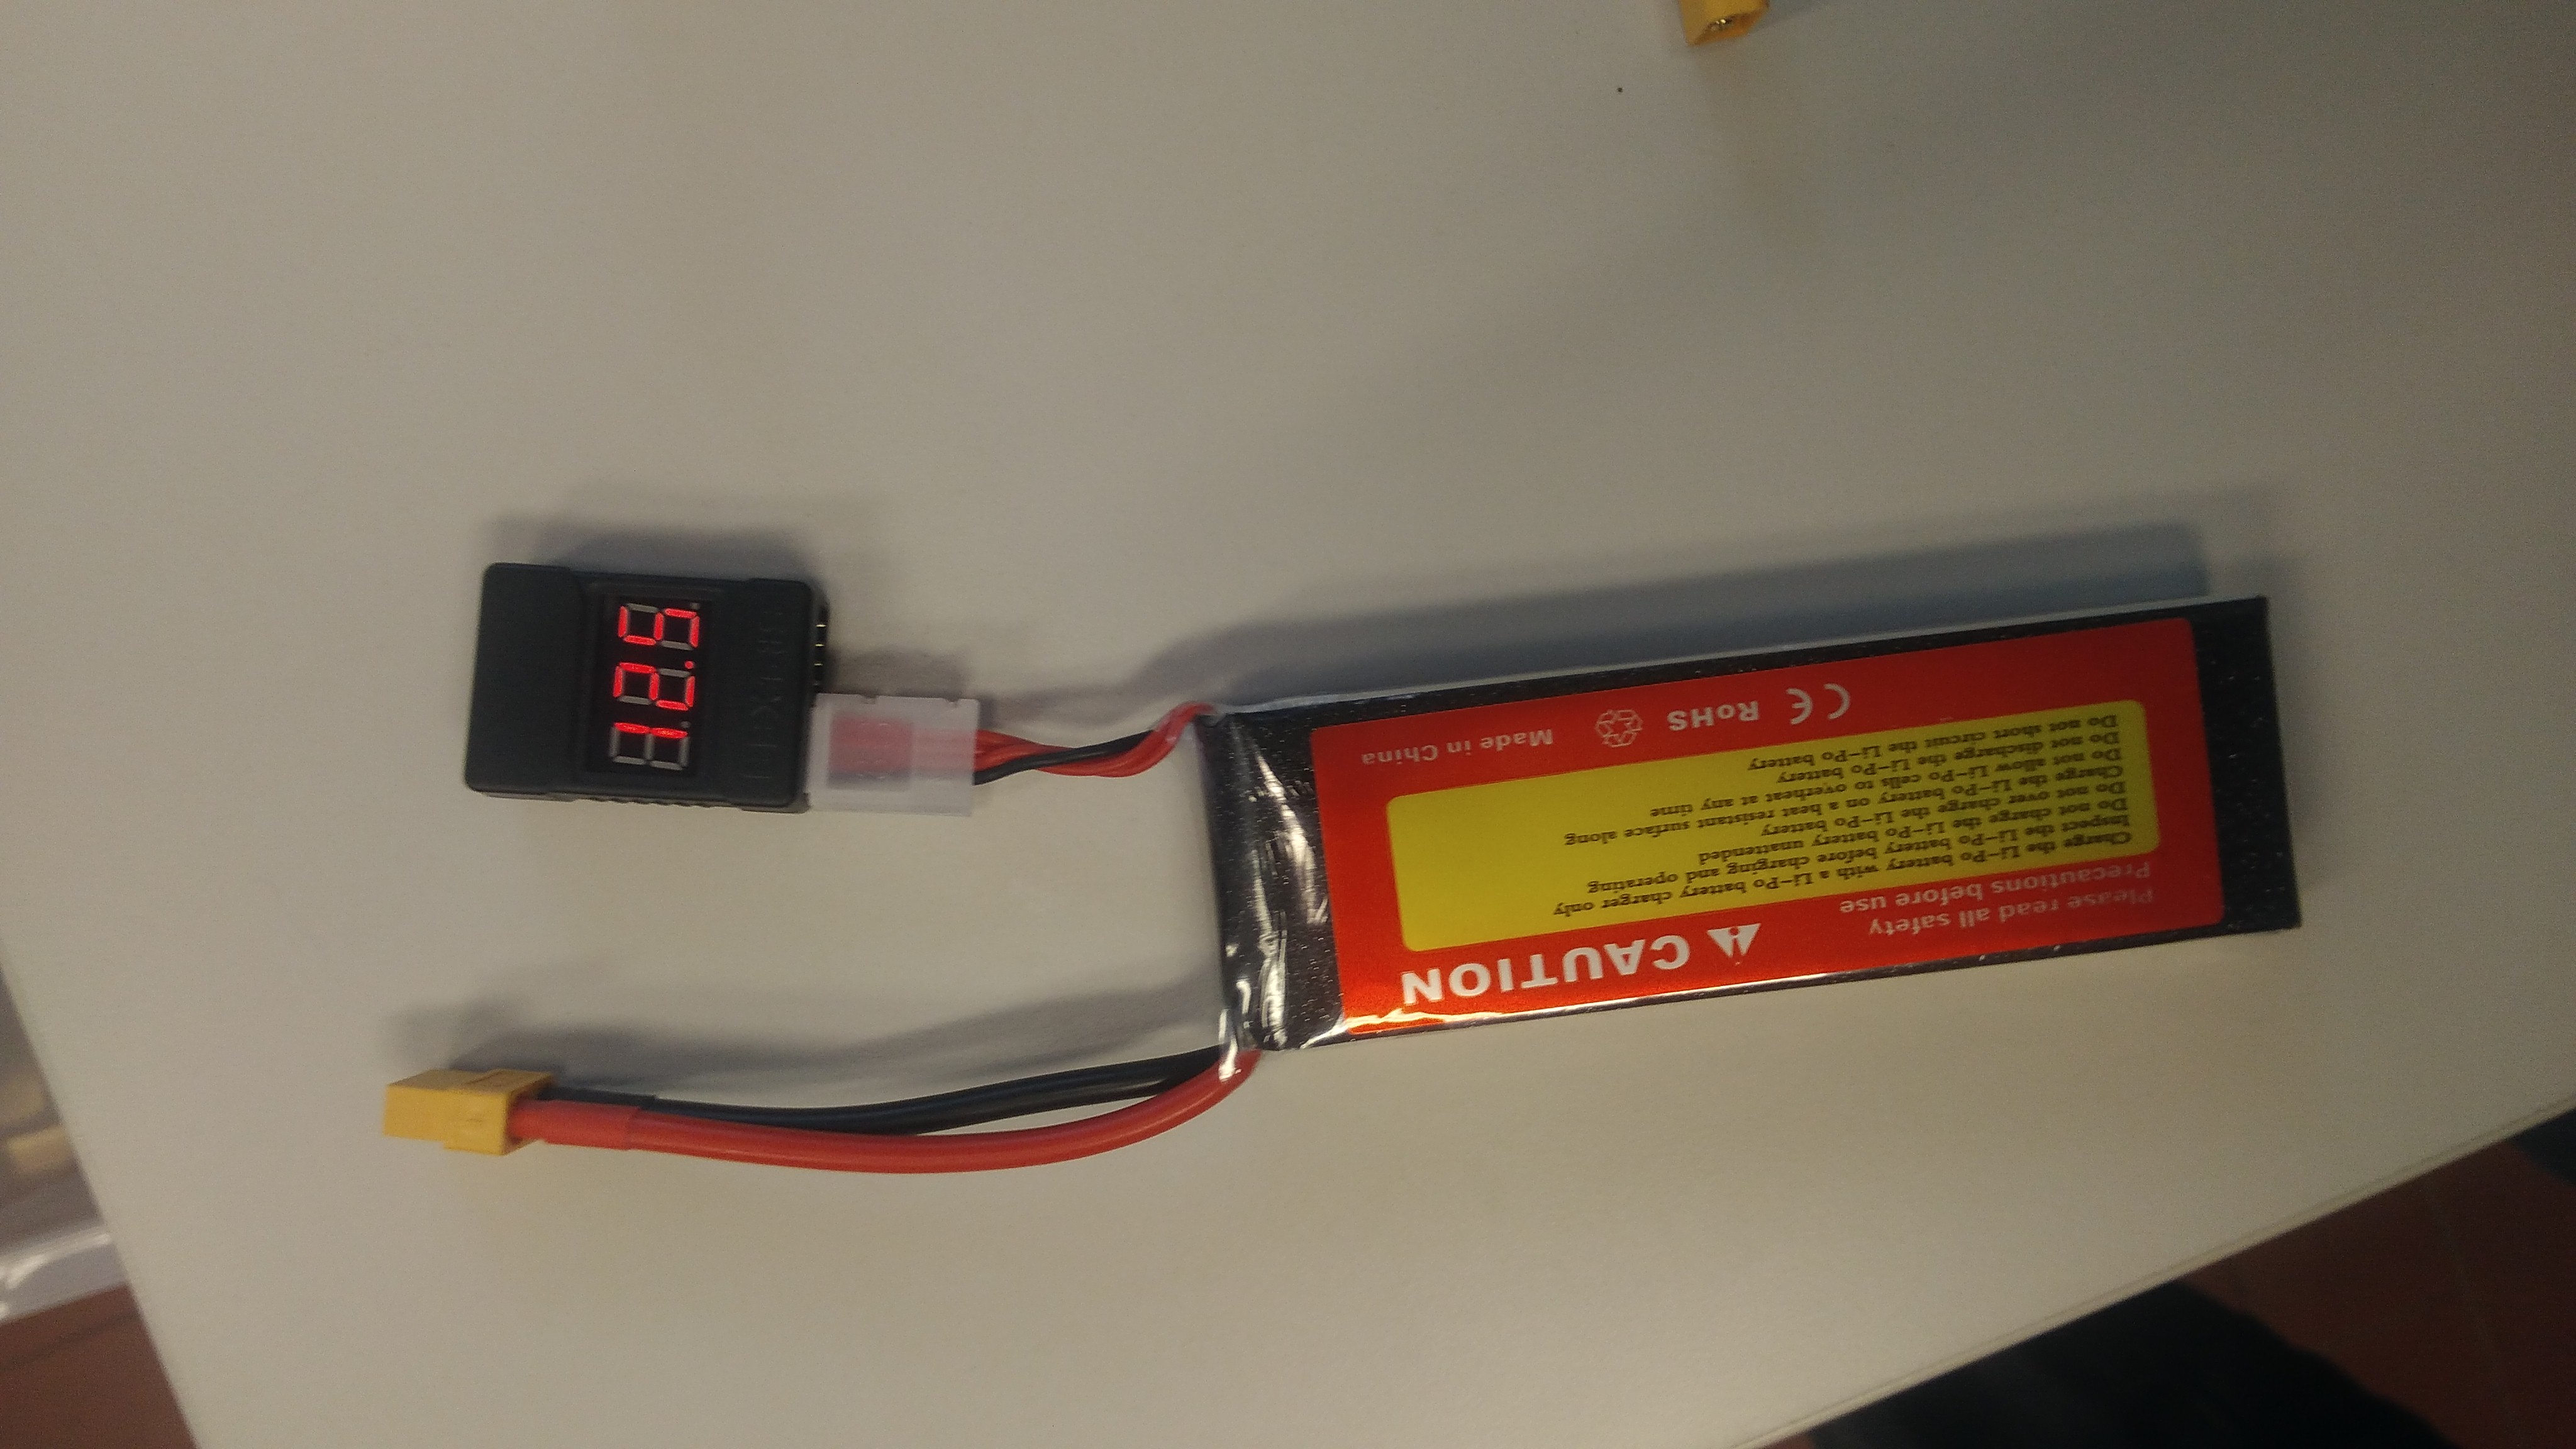
\includegraphics[width=.4\linewidth]{building/battery_voltage_monitor.jpg}

\subsection{Storing}
If you will not use the LiPo for a long time do not keep the batteries at full capacity. It would damage the LiPo. Use the mode storage ({\color{orange} To verify}) of the charger to discharge the battery.\\
The sequence of steps that have to be followed are:
\begin{enumerate}
    \item Power the battery charger.
    \item Set to "storage mode".
    \item Place the battery in the fire proof bag.
    \item Connect in the same way describe for charging.
    \item ???
    \item You can now disconnect the battery.
\end{enumerate}

{\color{blue} Add pictures of battery charging connection}

\section{Power Connections}
\begin{enumerate}
    \item Connect the power module to the Raspberry Pi.
    \item Connect the power module to the PDB connector.
    \item Connect a battery charger to the power module.
\end{enumerate}
The ESC should make some beeps when the Raspberry Pi is powered.
You can check if the Raspberry Pi is working by trying to connect via ssh.
{\color{orange} Elaborate}

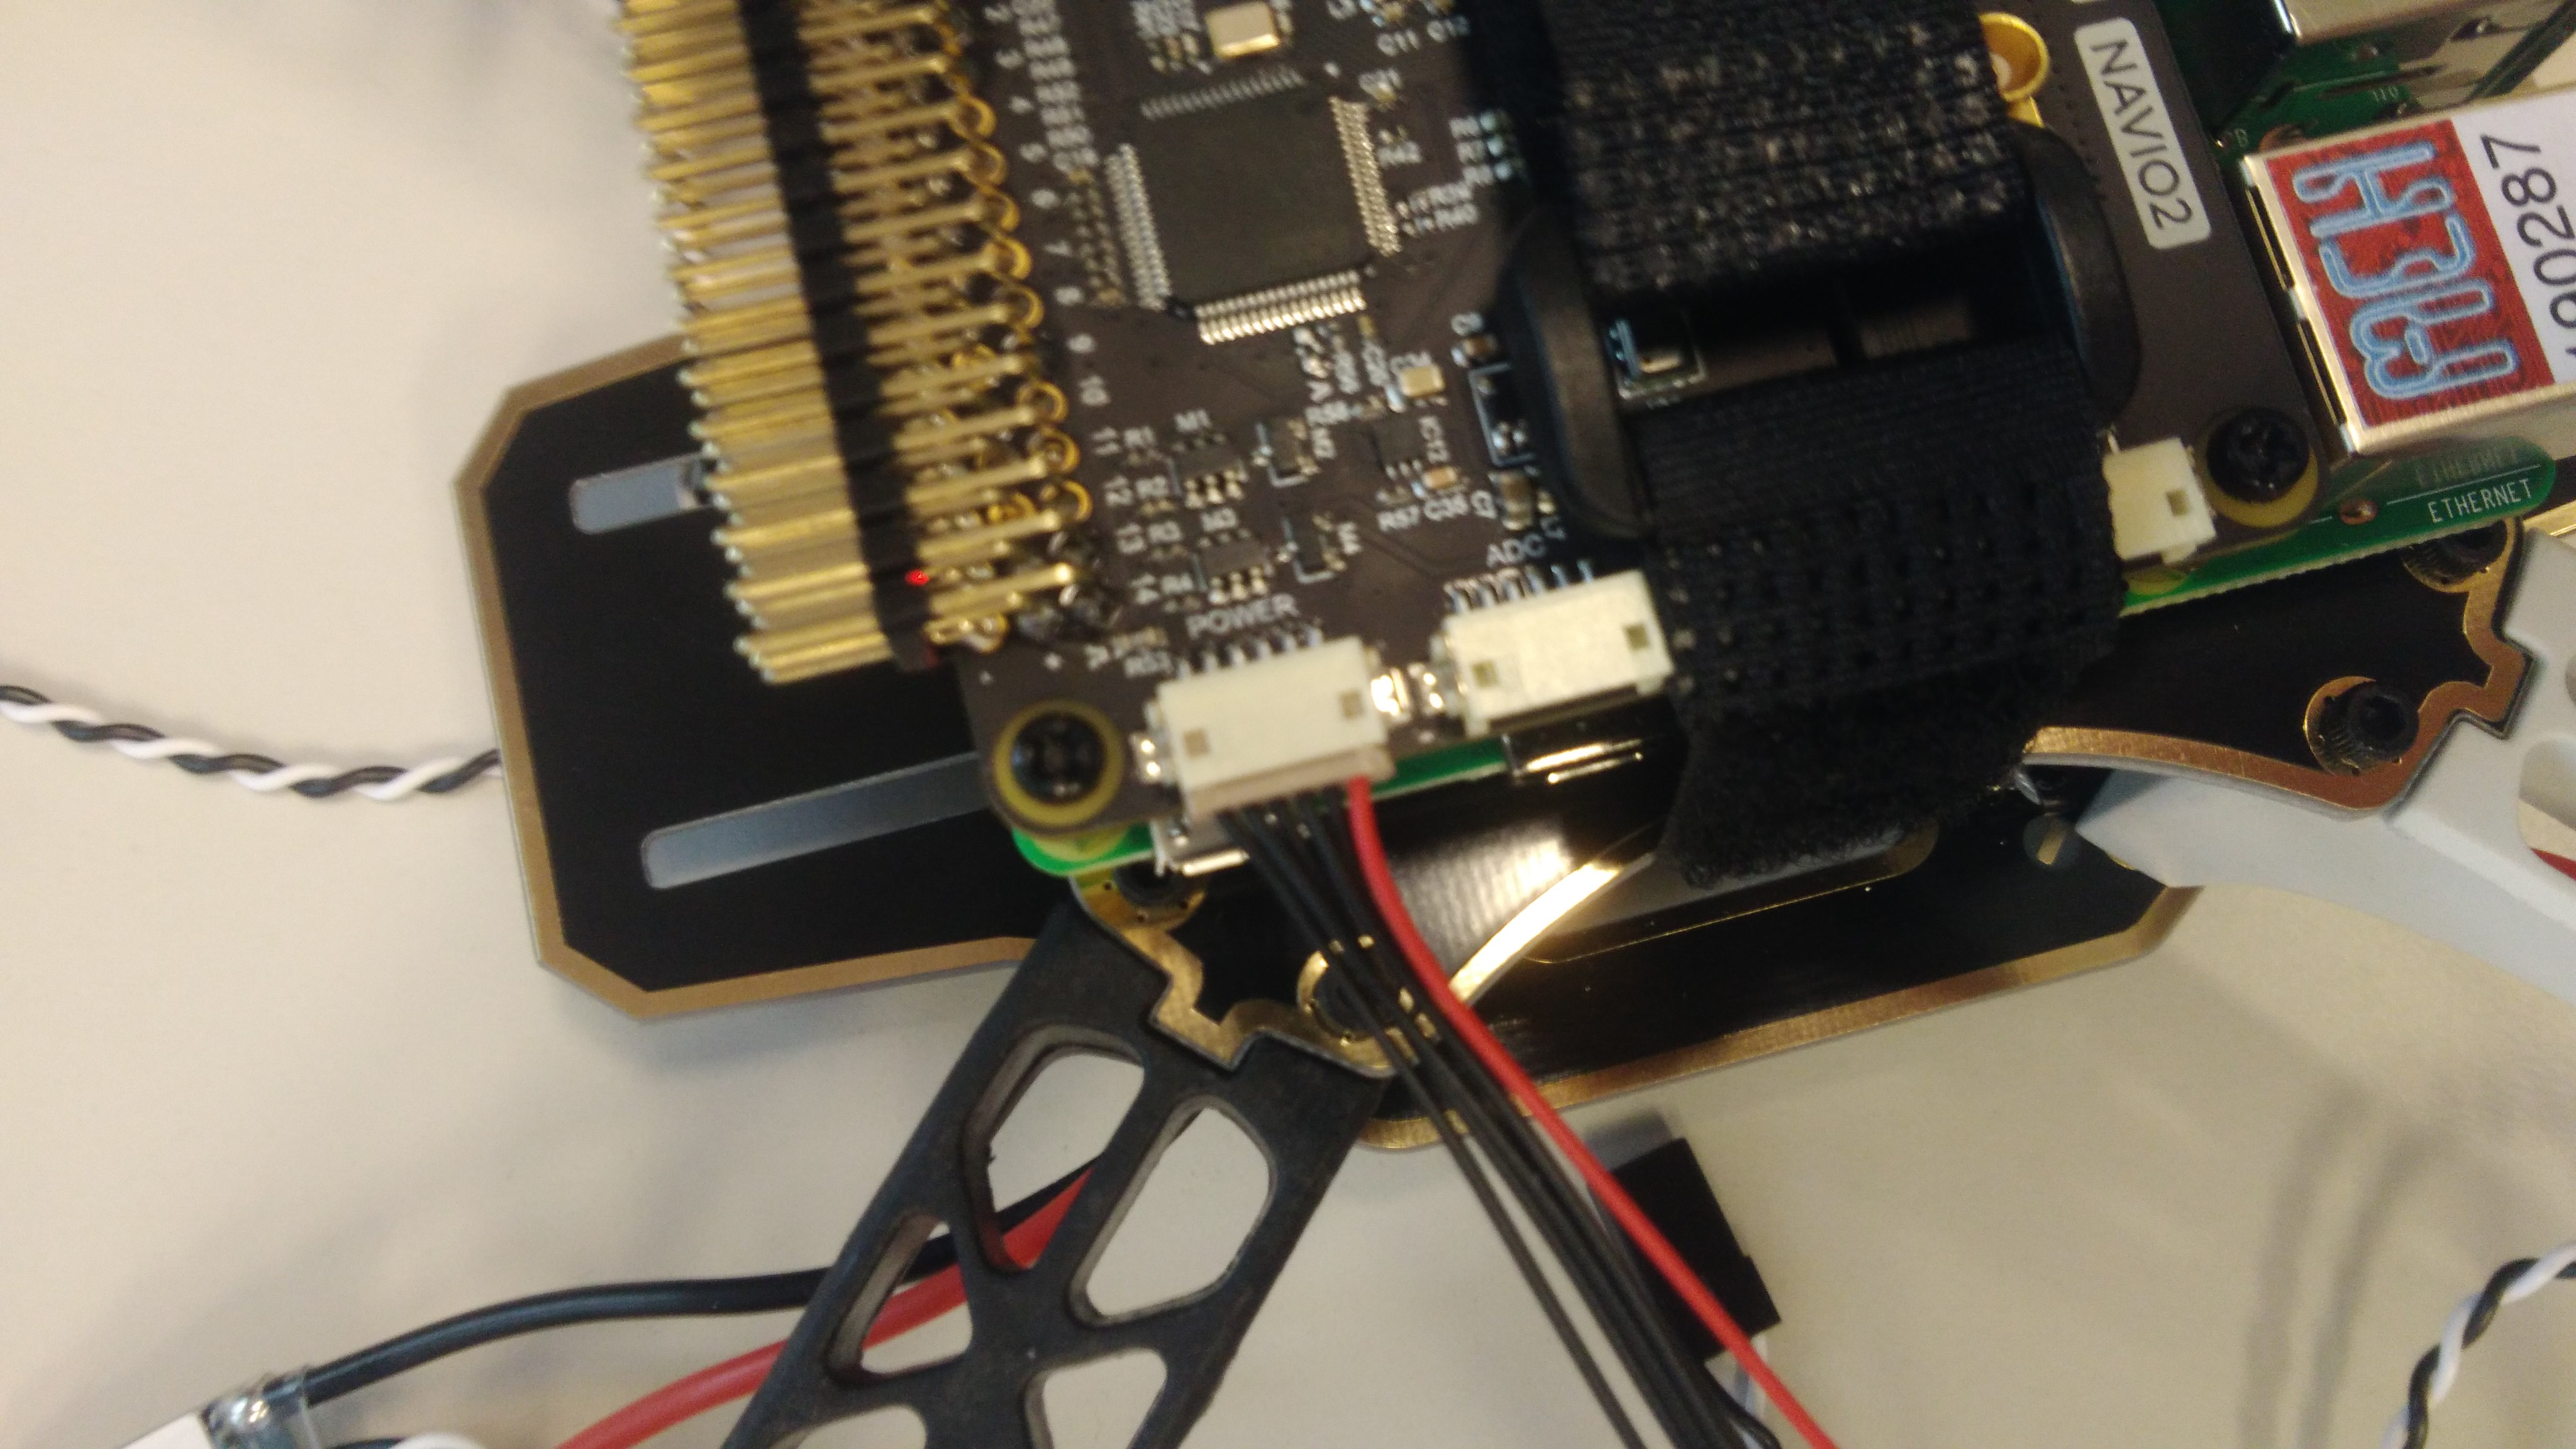
\includegraphics[width=.4\linewidth]{building/power_module_navio.jpg}
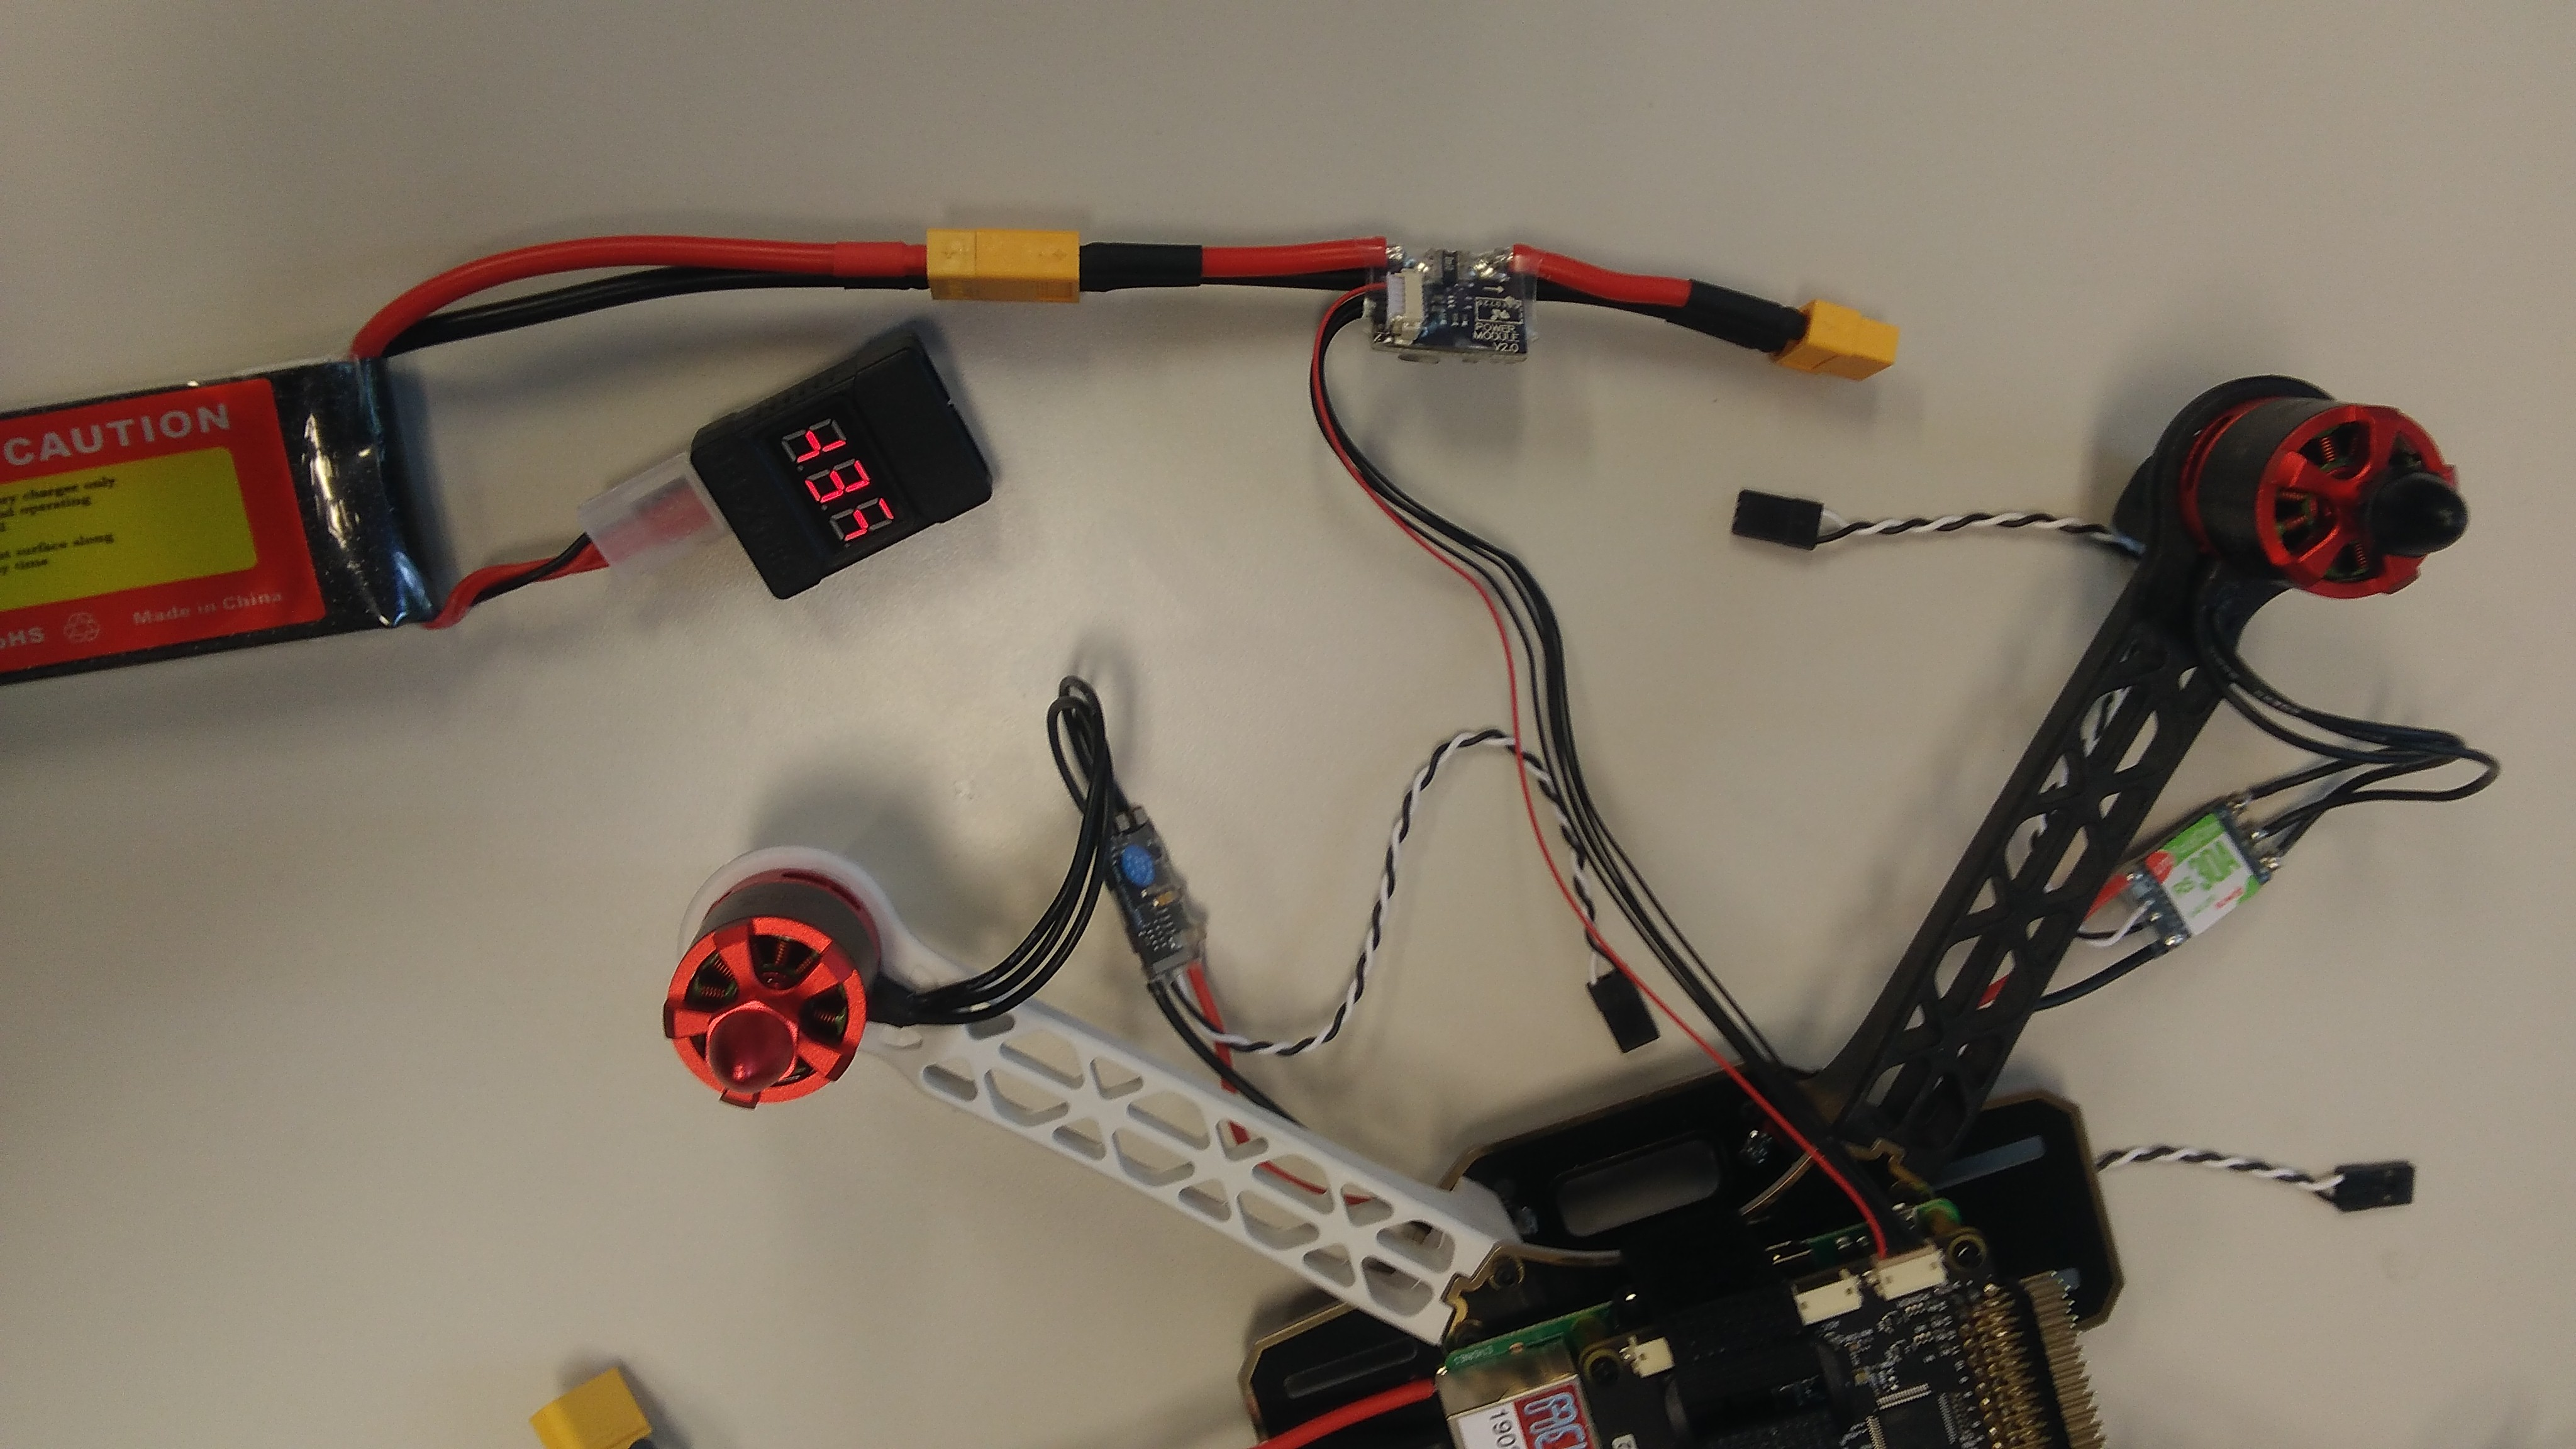
\includegraphics[width=.4\linewidth]{building/power_connections_bis.jpg}

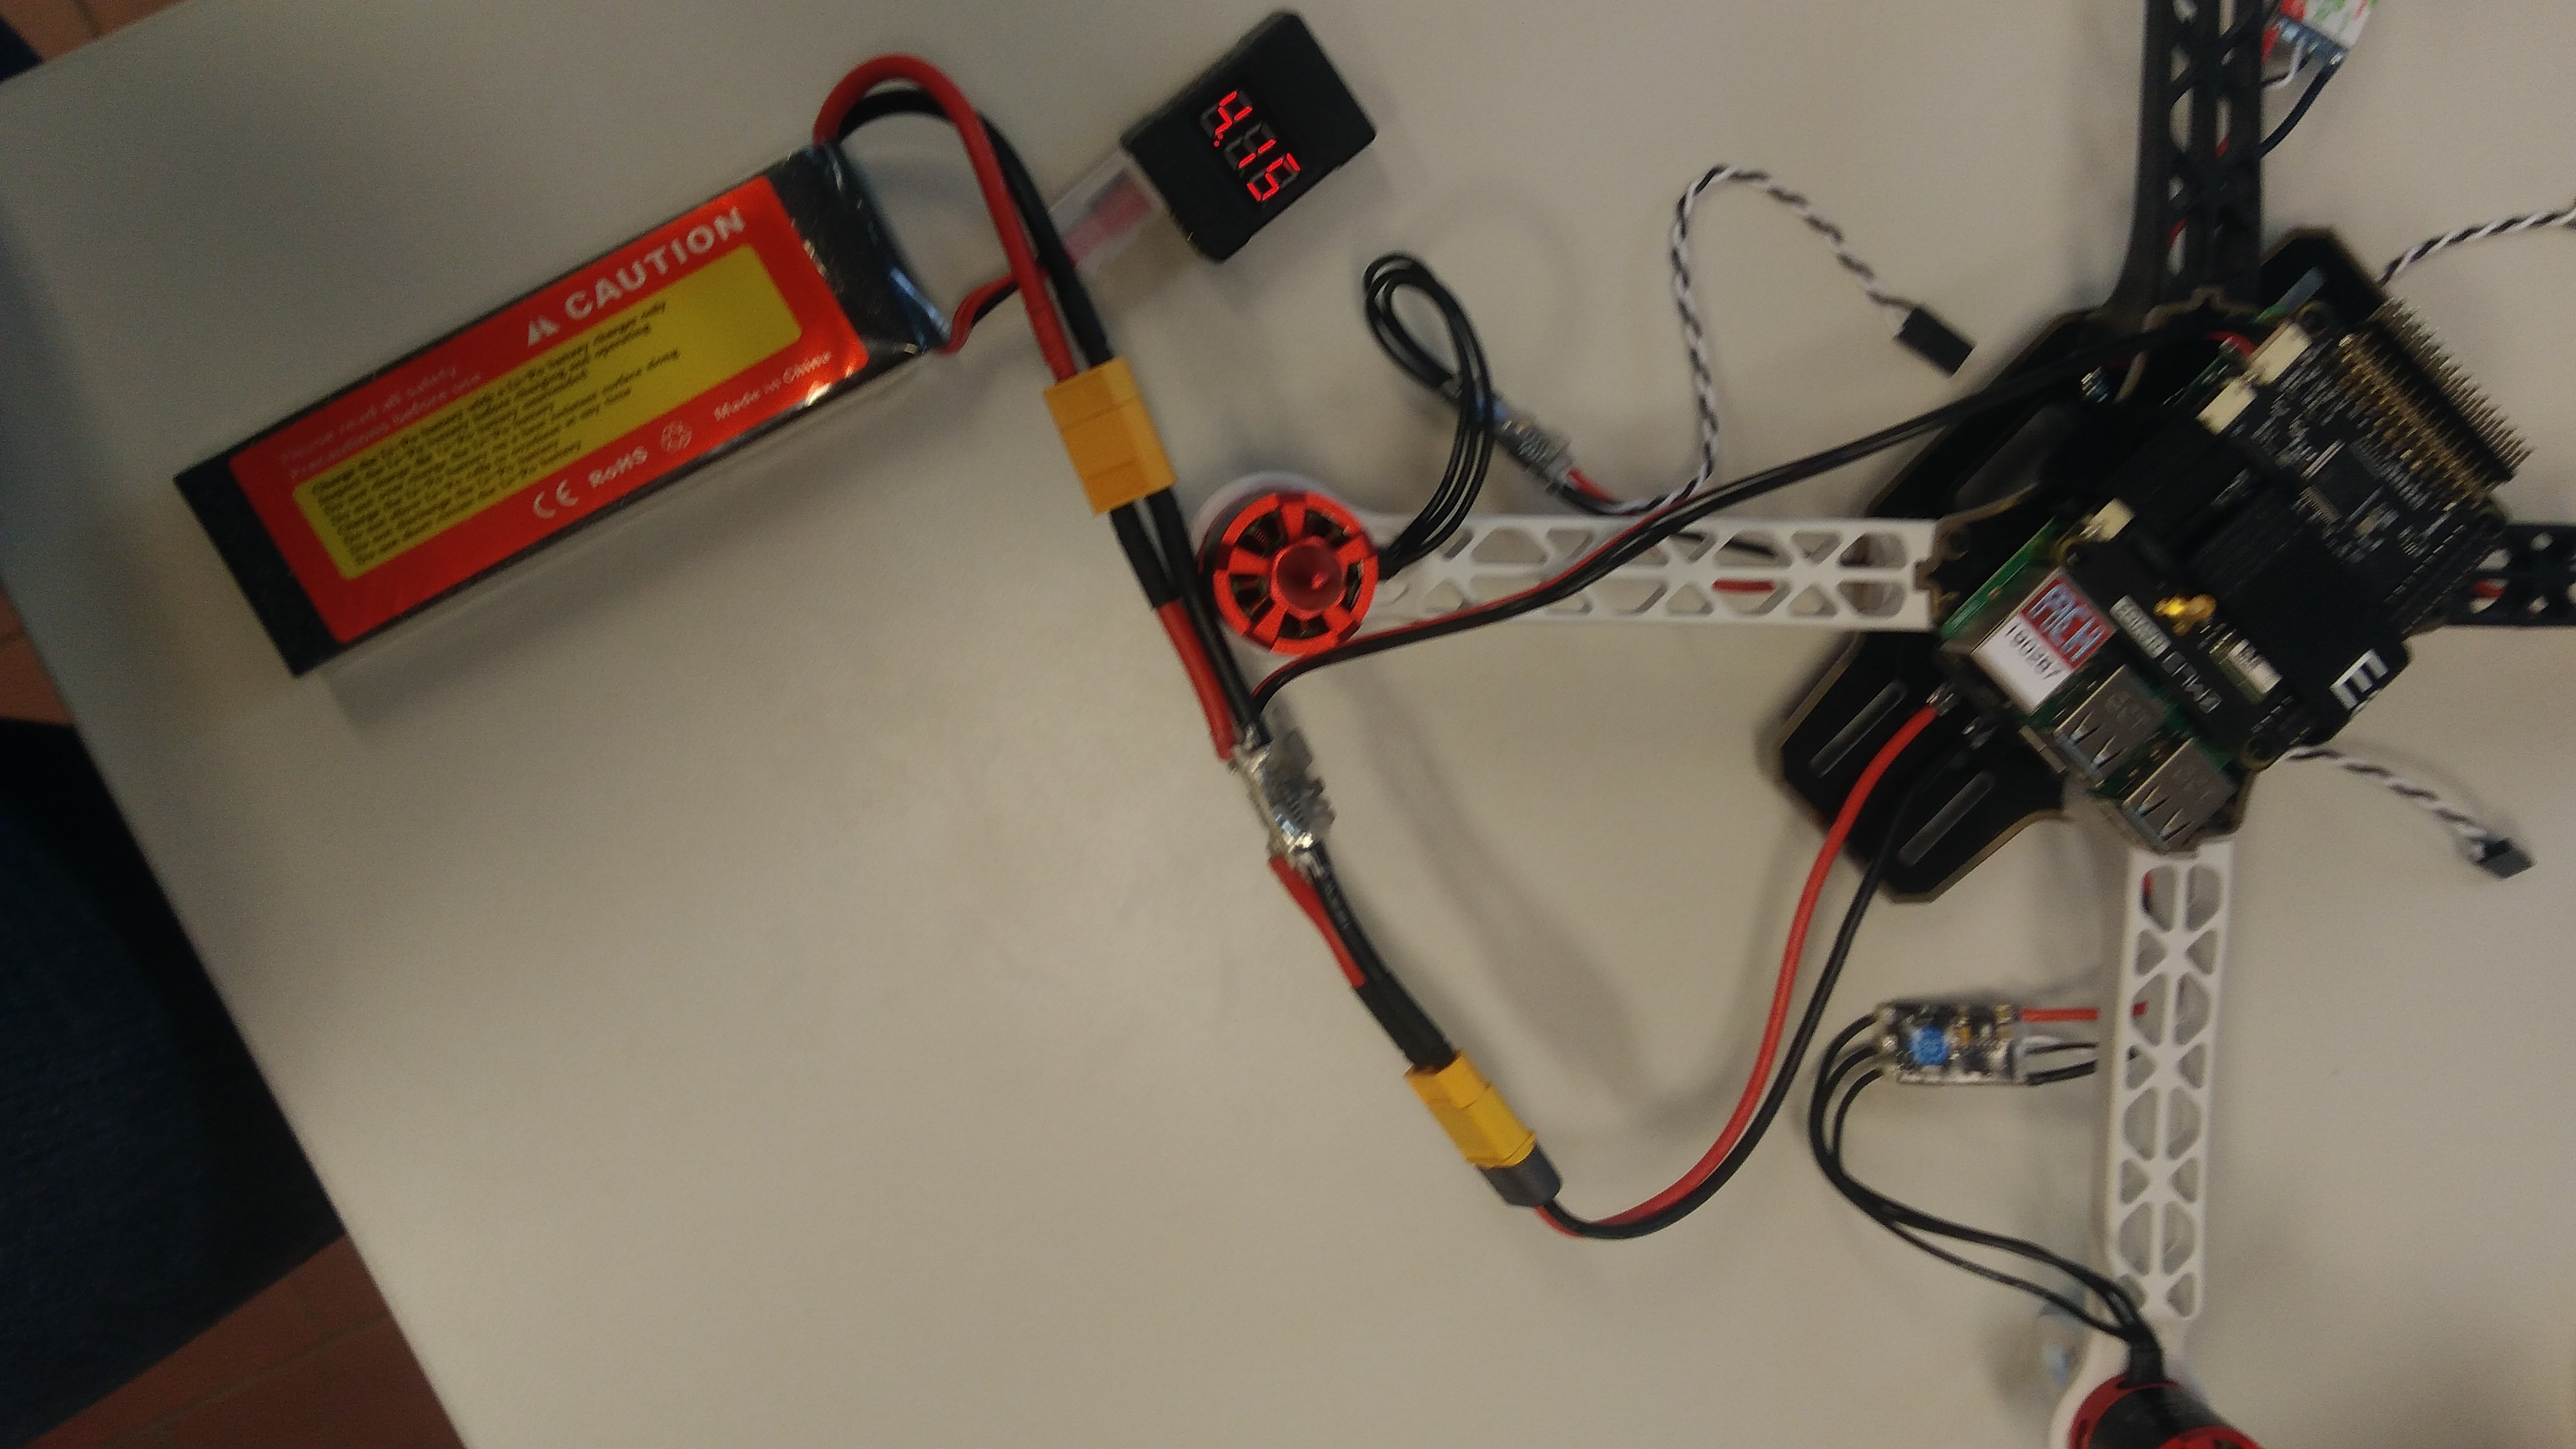
\includegraphics[width=.4\linewidth]{building/power_connections.jpg}

\section{Radio Control (RC)}
\subsection{Powering the Transmitter}
\begin{enumerate}
    \item Insert the batteries in the transmitter if not done yet.
    \item Make sure all switches are at their highest position and the throttle is at its lowest.
    \item Power on by toggling the power switch.
\end{enumerate}

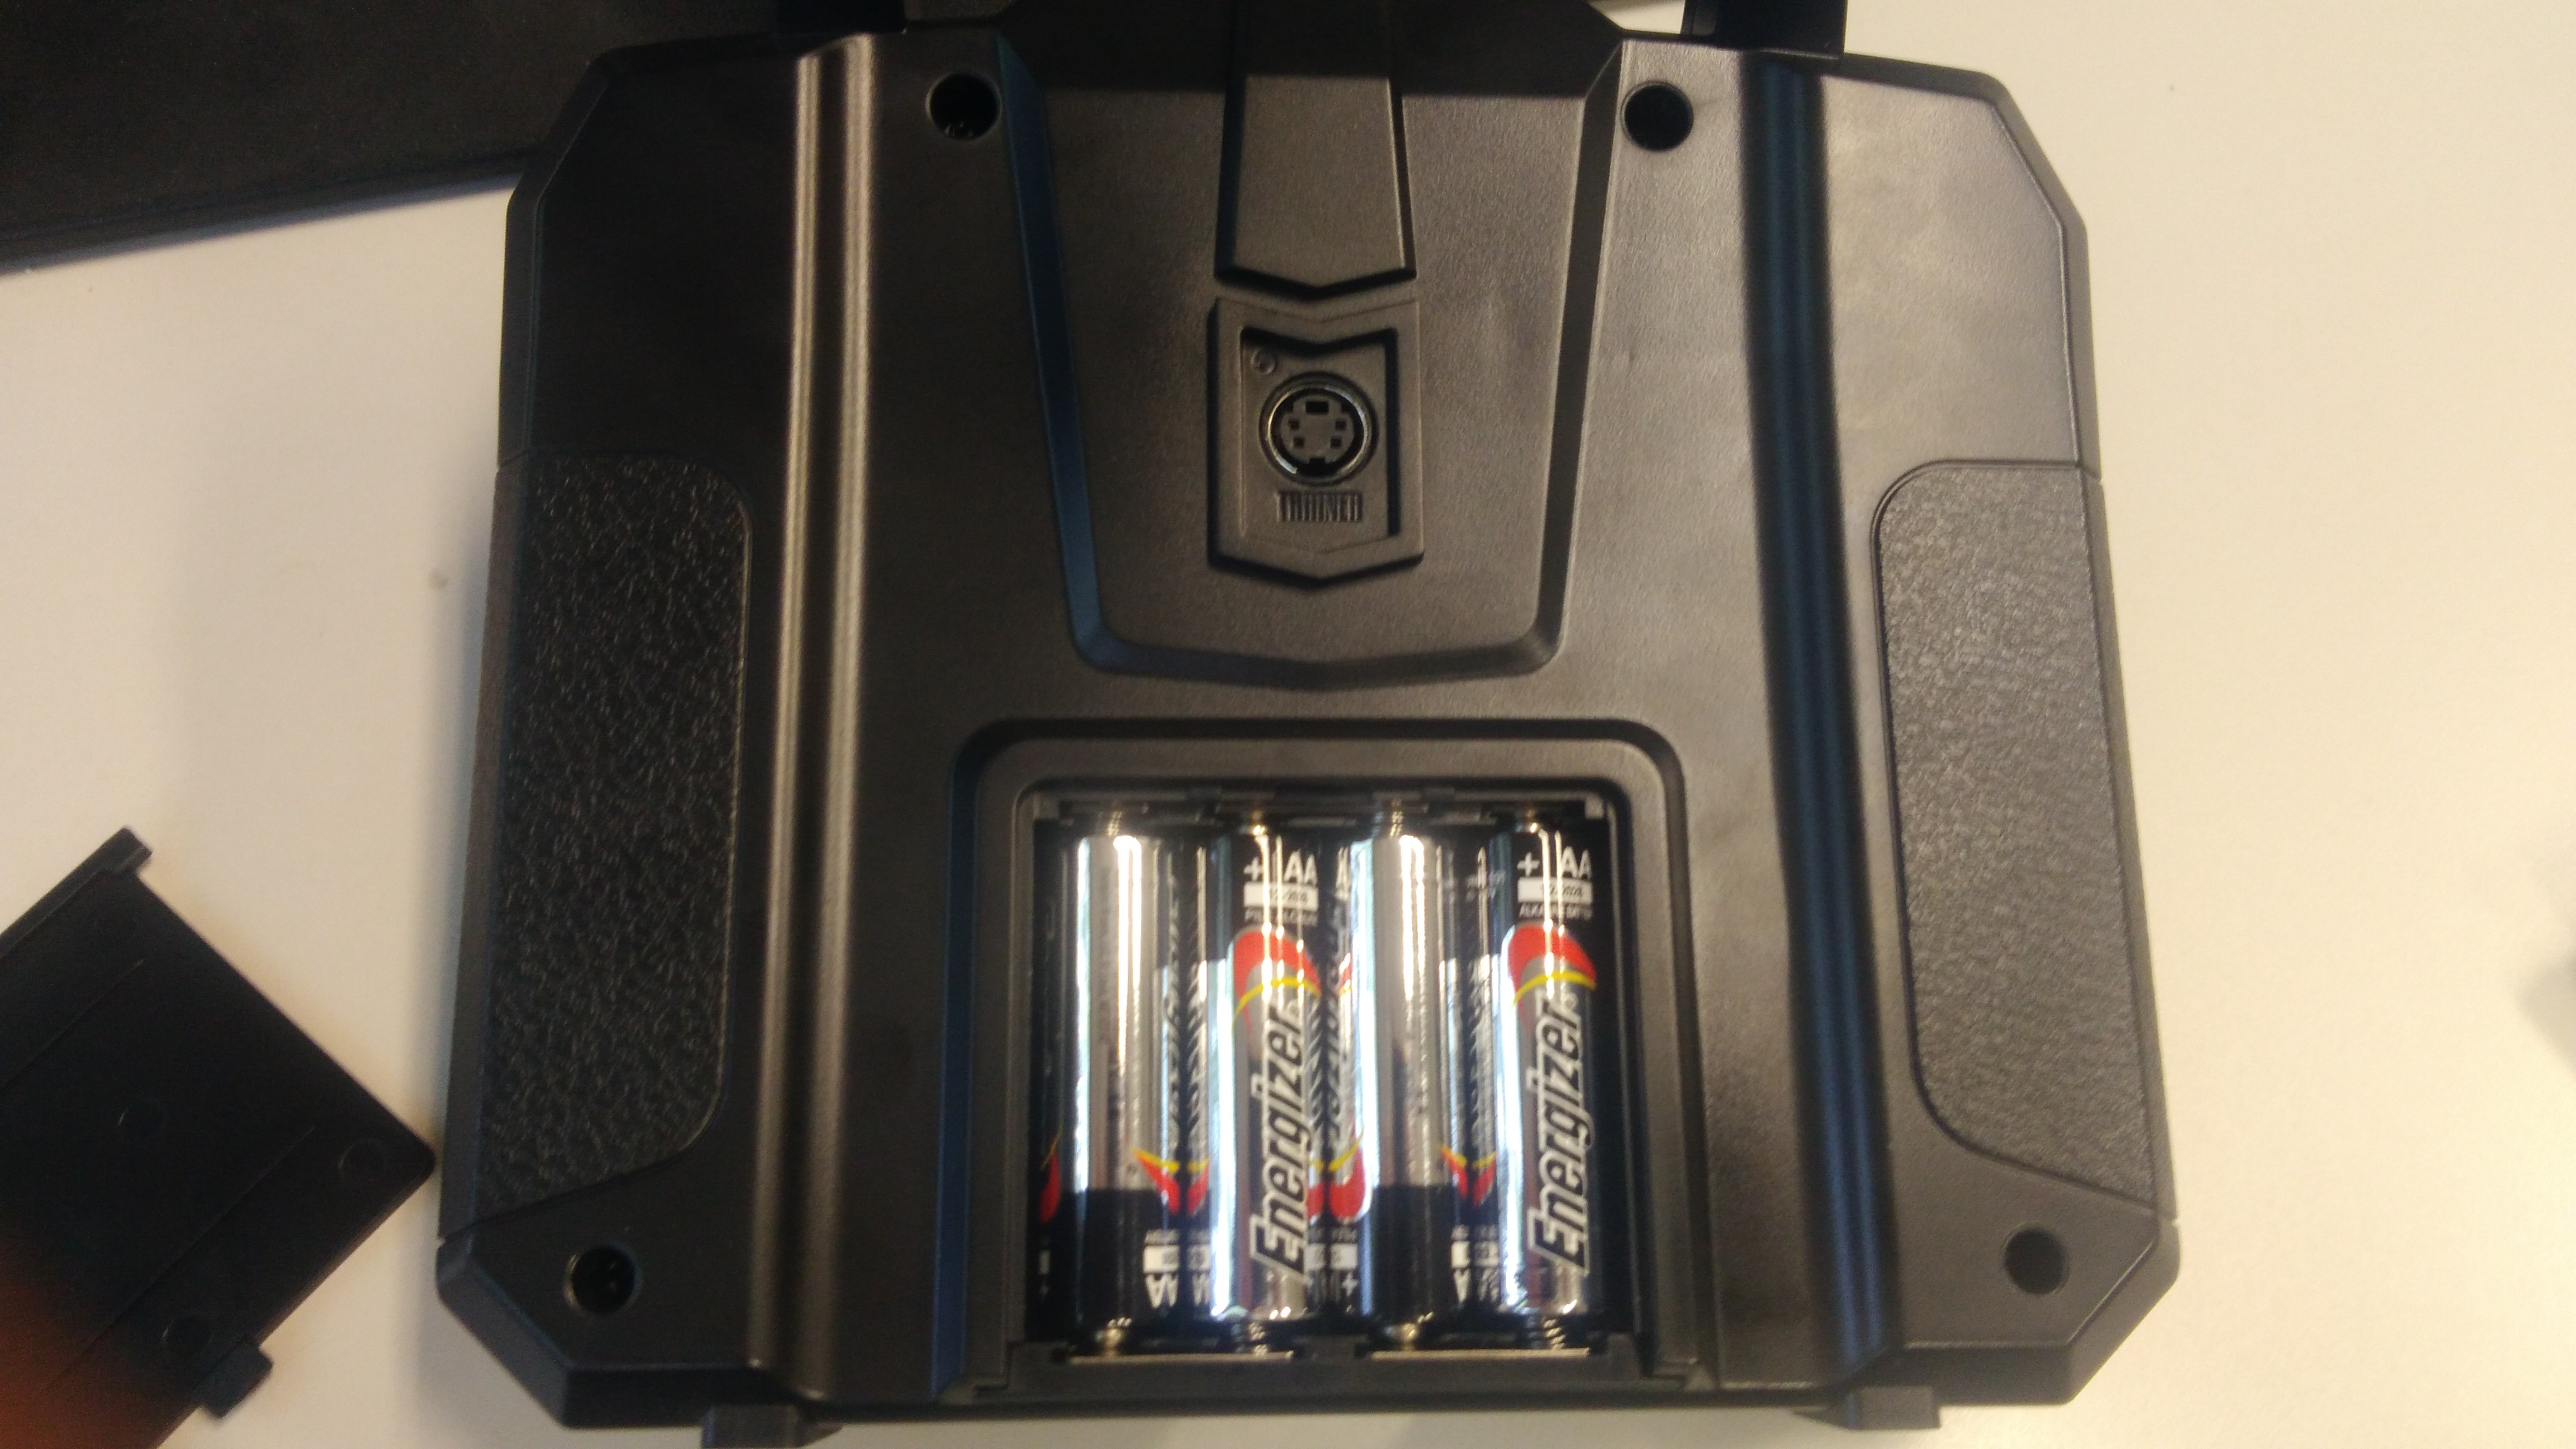
\includegraphics[width=.4\linewidth]{building/transmitter_battery.jpg}
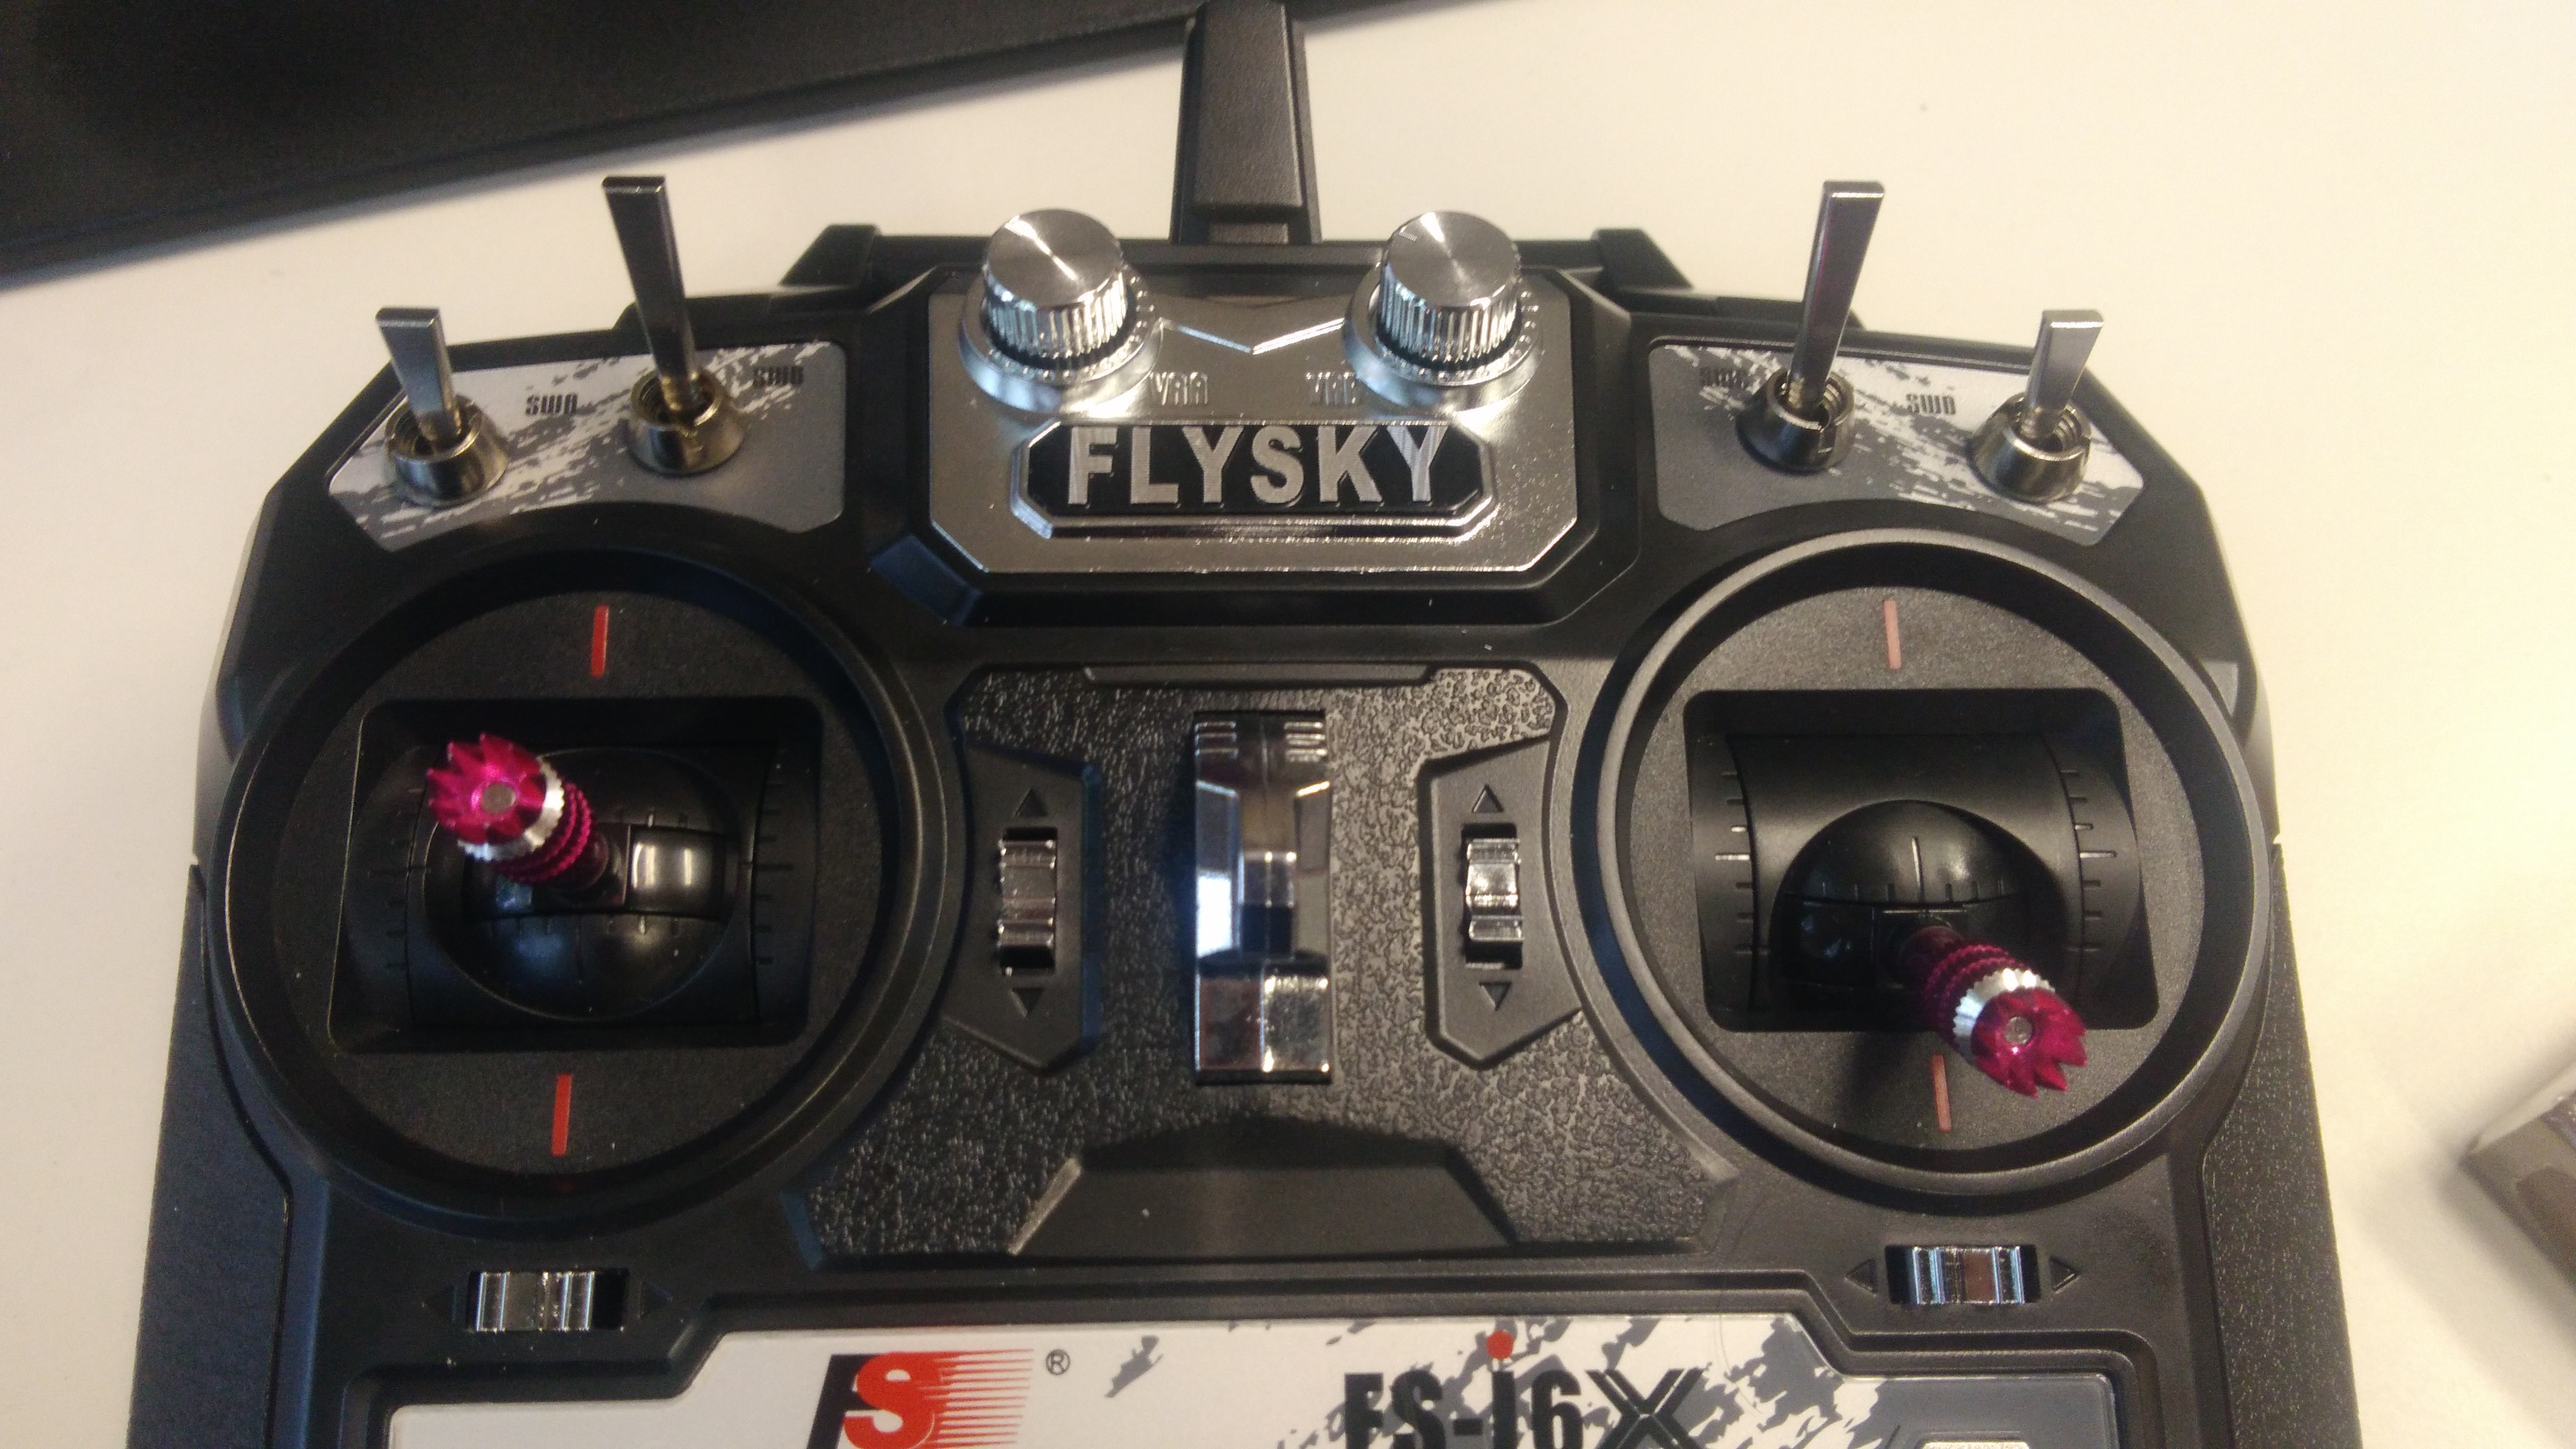
\includegraphics[width=.4\linewidth]{building/transmitter_controls.jpg}

{\color{blue} Add pictures of transmitter just powered on}

\subsection{Transmitter Navigation}
You can use \texttt{UP} and \texttt{DOWN} to move the cursor.
\texttt{OK} and \texttt{CANCEL} to select or return.
\texttt{CANCEL} can be used to cancel a modification with a single pressing or validate with a maintained pressing.

\subsection{Powering the receiver}
You can power the receiver by connecting ground to any pin the lowest row and Vcc to any pin of the middle row.
We chose to power the receiver with the Navio using \texttt{CH1/PPM} on the receiver and \texttt{PPM/SB} on the Navio. The Navio has to be powered to power the receiver.

\subsection{Binding the receiver to the transmitter}
\begin{enumerate}
    \item Power off the transmitter.
    \item Power the receiver.
    \item Connect the supplied bind cable to the B/VCC port on the receiver.
    \item Hold the \texttt{BIND KEY} while powering on the transmitter to enter bind mode. The transmitter will then display this.
\end{enumerate}


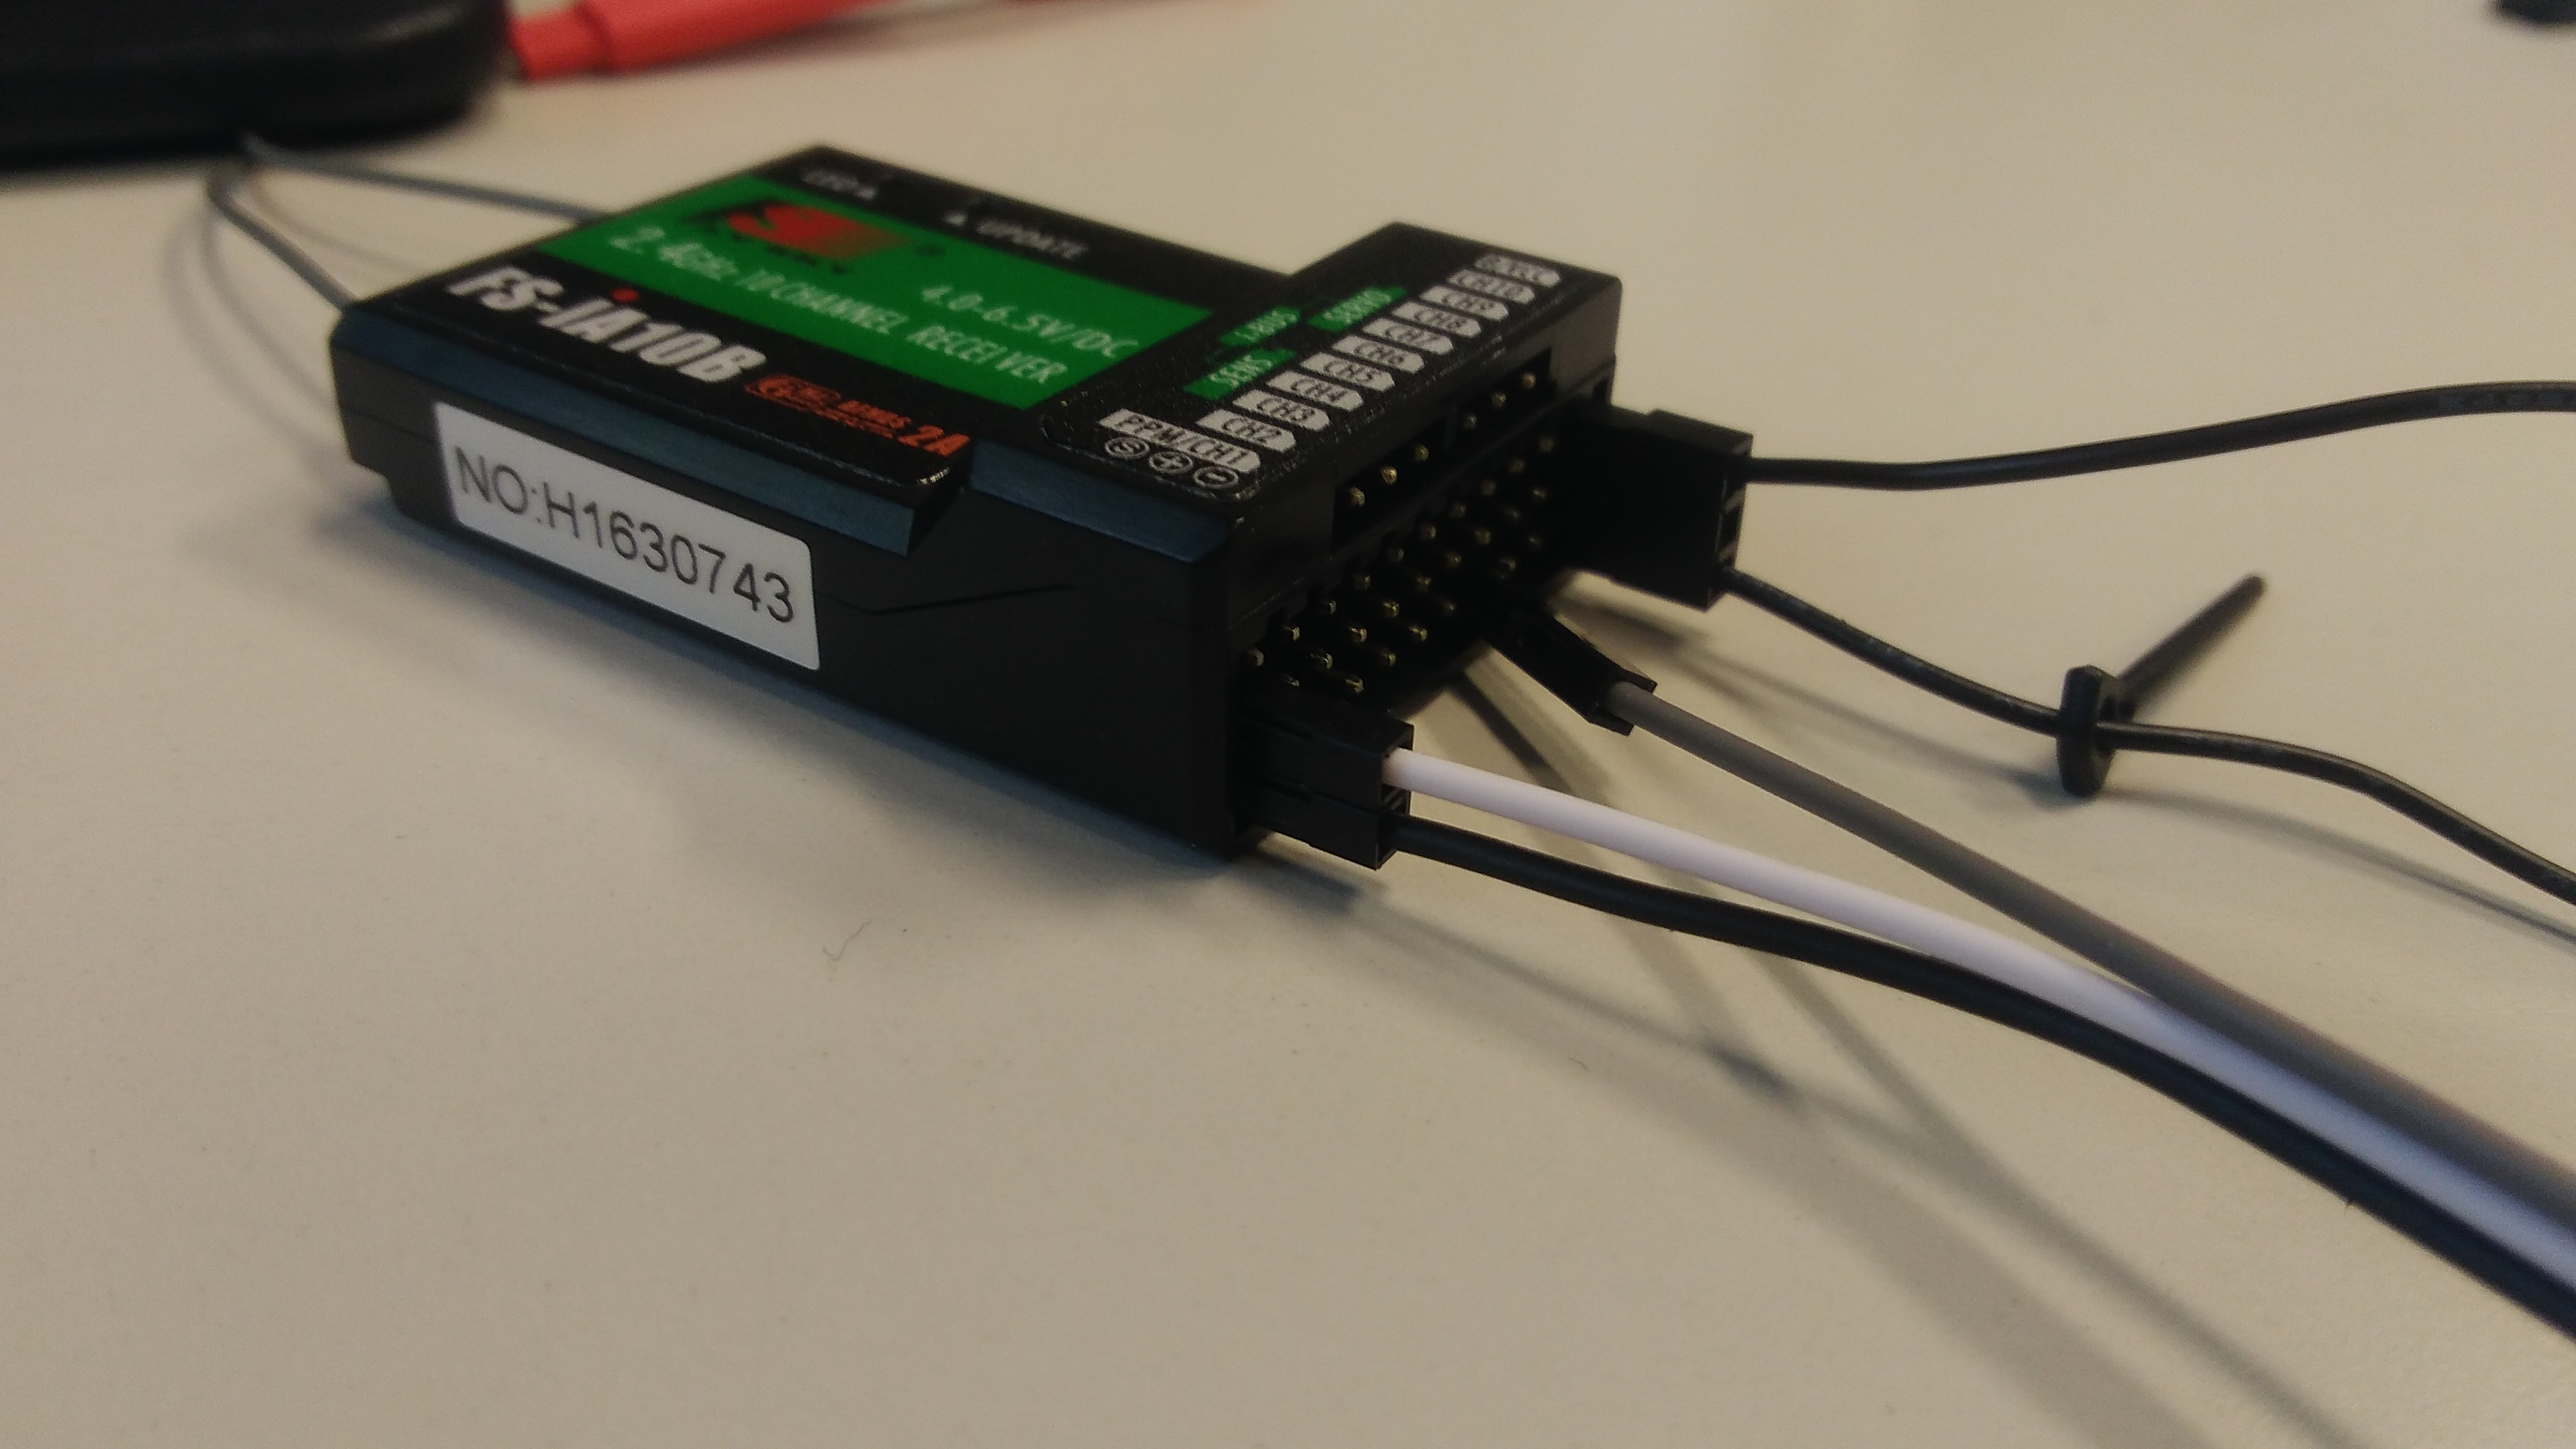
\includegraphics[width=.4\linewidth]{building/receiver_bind.jpg}
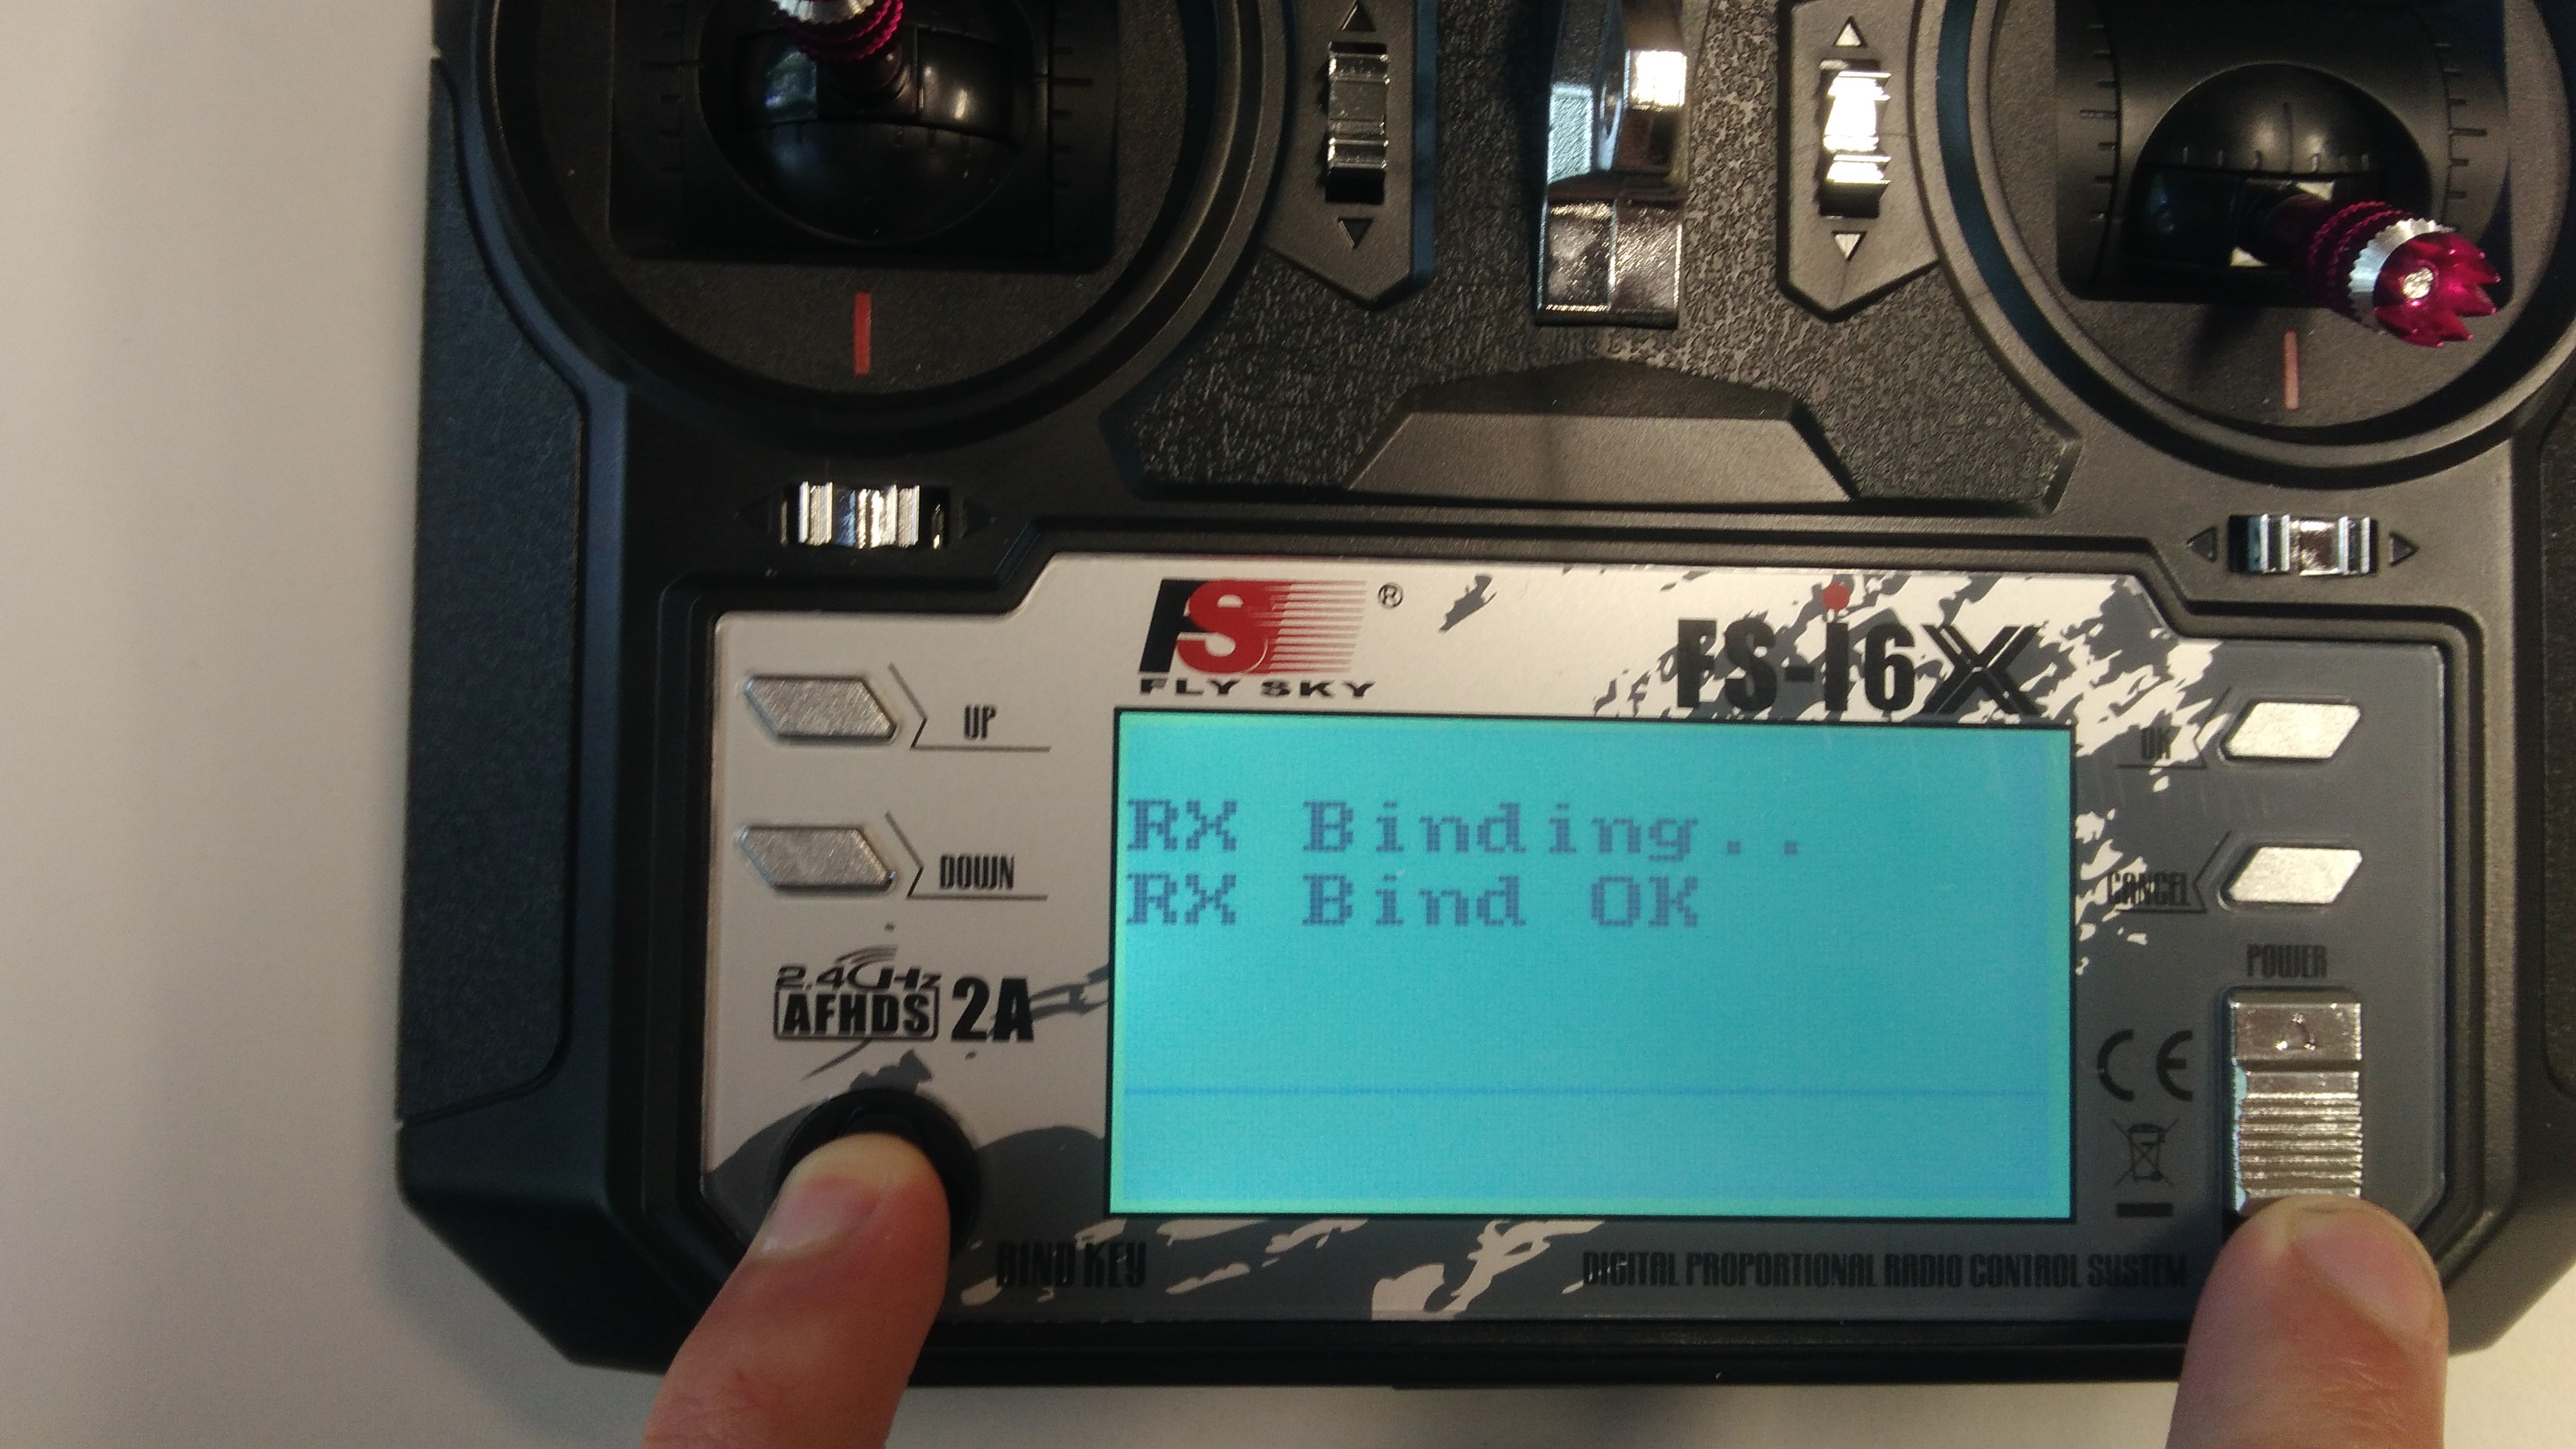
\includegraphics[width=.4\linewidth]{building/transmitter_binding.jpg}

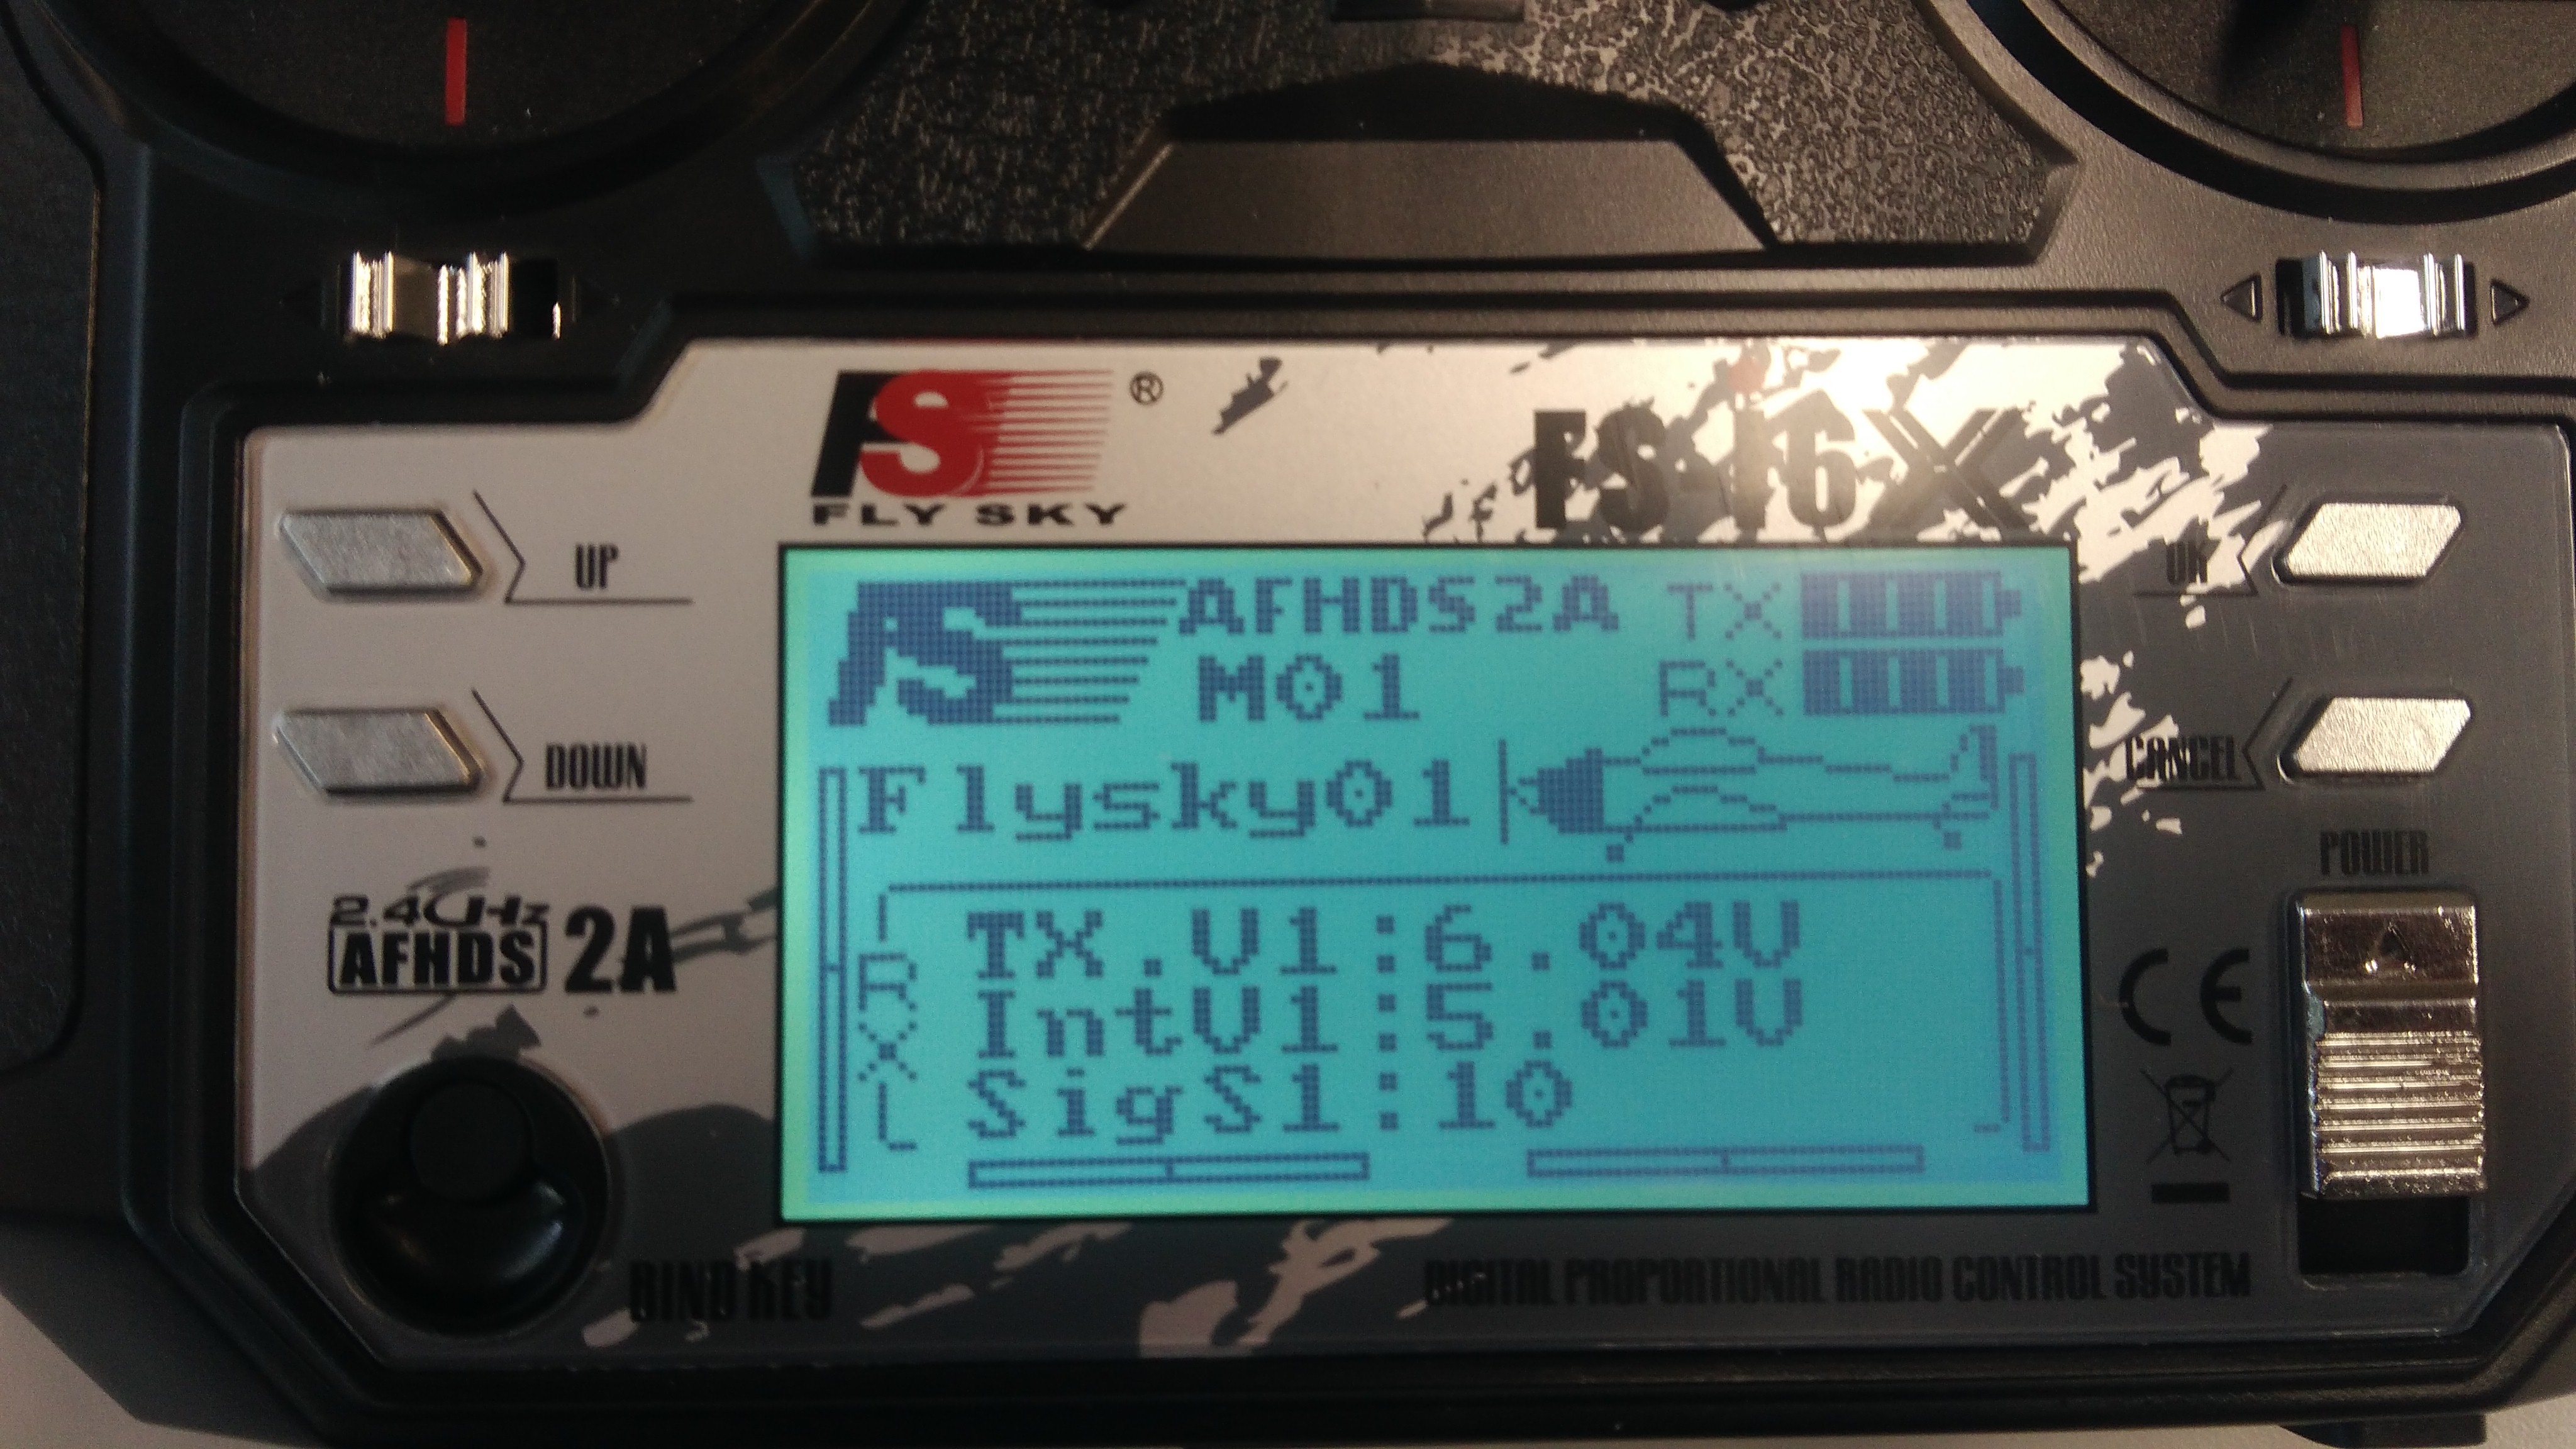
\includegraphics[width=.4\linewidth]{building/transmitter_receiver_detected.jpg}

\subsection{Changing the output mode of the receiver}
The \texttt{PWM} mode sends the PWM signal to each channel on the receiver. You can text your ESC with this mode.

The \texttt{PPM} mode send all the signals to the channel 1 of the receiver. This reduces the number of cables to connect to the flight controller. It is the solution used to control the Navio.

\begin{enumerate}
    \item Power on the transmitter.
    \item Maintain OK pressed until the menu appears.
    \item Select \texttt{System setup}
    \item Select \texttt{RX setup}
    \item Select \texttt{Output mode}
    \item You can choose between the \texttt{PWM} and \texttt{PPM} mode for the receiver, the rest of the option is not use in this project. Maintain press \texttt{Cancel} to validate.
    \item Press \texttt{Cancel} 3 times to return to the start-up screen.
\end{enumerate}

\subsection{Configuring Auxiliary channels}
\paragraph{Activating switches}
\begin{enumerate}
    \item Go to \texttt{MENU/System setup/Aux. switches}.
    \item Choose which switches and how many auxiliary channels to activate.
    \item Validate by maintaining press \texttt{CANCEL}.
\end{enumerate}

\paragraph{Allocating switches to channels}
You can allocate a switch to channel you have activated.
\begin{enumerate}
    \item Go to \texttt{MENU/Functions setup/Aux. channels}.
    \item Choose which switch go to which channel.
    \item Validate by maintaining press \texttt{CANCEL}.
\end{enumerate}

\section{ESC}
The following section will expain how to setup the ESC.
Do it one motor at a time on all motors.

Do not put propellers on the motors! It is really dangerous when the motor are not calibrated.
\subsection{Testing Motor}

\begin{enumerate}
    \item Set the \texttt{PWM} output mode.
    \item Power of the transmitter.
    \item Plug on the receiver \texttt{CH3} the ESC with the white cable on top.
    \item Power the receiver on.
    \item Power the transmitter on.
\end{enumerate}
You can now control the speed of the motor connected to the receiver. But it is possible that when you move the throttle stick a little the motor does not react to it. That is where calibration comes in. You also want to check the spin direction of the motor. So do not change the cabling for now.

\subsection{Calibrating}
The calibration of the ESC consist in giving the minimum and maximum position of the transmitter throttle stick to the ESC so that the maximum and minimum throttle correspond to the real minimum and maximum throttle.

\begin{enumerate}
    \item Unplug the battery of the drone.
    \item Power the transmitter on.
    \item Place the throttle to the highest position.
    \item Plug the battery of the drone.
    \item Wait for the beeps to stops.
    \item Place the throttle to the lowest position.
    \item Wait for the beeps to stops.
\end{enumerate}
You now have a calibrated motor.


\subsection{Motor Spin Direction}
Now, you will check if the motors are rotating in the right direction.

\begin{enumerate}
    \item Increase the throttle a little to make the motor spin slowly.
    \item Check if the motor spin in the right direction.
    \item If the motor spin direction is not the right one. Inverse to cable of the motor connected to the ESC.
\end{enumerate}

You now have a motor with the right direction speed.

\section{Navio connection}
Connect the receiver and the ESC in the right order.
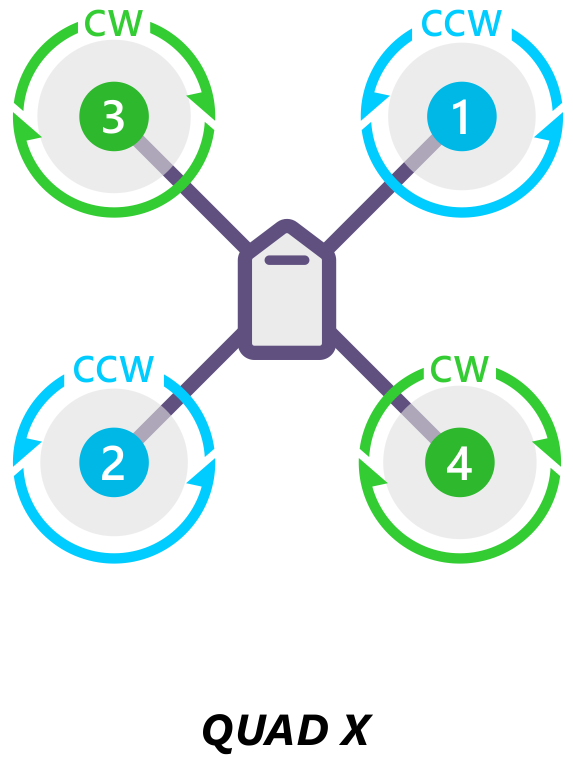
\includegraphics[width=.4\linewidth]{building/motororder_quad_x_2d.png}

\section{Securing every part}
Zip ties and scratch was used.


\section{Leashing the drone}
Leashing the drone is useful to restrict the drone flight space. It is particularly useful when you are testing new maneuvers.
\begin{enumerate}
    \item Attach the leash under the drone.
    \item Unroll enough rope for the drone to fly.
    \item Attach the leash to a weight
\end{enumerate}
